\documentclass{mynotes}

\usepackage{amsmath,amsfonts,amsthm,amssymb}
\usepackage{bm}
%\usepackage{indentfirst}
\usepackage{algorithm}
\usepackage{algpseudocode}
\usepackage{emoji}

\usepackage{subcaption}

\usepackage{tikz}

\PassOptionsToPackage{hyphens}{url}

\theoremstyle{definition}
\newtheorem{example}{Ví dụ}

\renewcommand*{\proofname}{Chứng minh}
\counterwithin*{example}{chapter}

\renewcommand*{\chaptername}{Chương}
\renewcommand*{\appendixname}{Phụ lục}
\renewcommand*{\contentsname}{Mục lục}
\renewcommand*{\figurename}{Hình}
\renewcommand*{\tablename}{Bảng}

\newcommand{\MC}{\mathcal{C}}
\newcommand{\FF}{\mathbb{F}}
\newcommand{\NN}{\mathbb{N}}
\newcommand{\ZZ}{\mathbb{Z}}
\newcommand{\RR}{\mathbb{R}}
\newcommand{\II}{\mathbb{I}}
\newcommand{\CC}{\mathbb{C}}

% affine space
\newcommand{\Vv}{\mathcal{V}}
\newcommand{\Aa}{\mathcal{A}}

\DeclareMathOperator{\Ima}{im}
\DeclareMathOperator{\tr}{tr}
\DeclareMathOperator{\rank}{rank}
\DeclareMathOperator{\sign}{sign}
\DeclareMathOperator{\spa}{spa}
\DeclareMathOperator{\sgn}{sgn}
\DeclareMathOperator{\lb}{label}

\setlength{\parskip}{4pt}
\addbibresource{references.bib}

\setcounter{tocdepth}{1}

\setlist[itemize,enumerate]{noitemsep,nosep,leftmargin=0pt,itemindent=\parindent}

\begin{document}

\tableofcontents

\chapter{Ma trận}

Trong các bài viết của về đại số tuyến tính:

\begin{itemize}
    \item Vector sẽ được ký hiệu bởi chữ thường in đậm (ví dụ $\bm{v}, \bm{x}, \ldots$)​; 
    \item Ma trận sẽ được ký hiệu bởi chữ hoa in đậm (ví dụ $\bm{A},\ \bm{B}, \ldots$​);
    \item Các đại lượng vô hướng (số) được ký hiệu bởi chữ thường không in đậm (ví dụ $x_1,\ N,\ t, \ldots$).
\end{itemize}

\section{Định thức và hạng ma trận}

\subsection*{Định thức ma trận}

\begin{definition}[Nghịch thế]
    Cho tập hợp $A = \{1, 2, \cdots, n\}$ và xét hoán vị $\sigma$ trên ​$A$. Ta gọi hai phần tử $i$​ và $j$​ tạo thành \textbf{nghịch thế} (inversion) nếu $i < j$​ và $\sigma(i) > \sigma(j)$.

    Đặt $\sigma = \{k_1, k_2, \cdots, k_n\}$​ là một hoán vị của $A$​. Ta ký hiệu \[ P\{k_1, k_2, \cdots, k_n\} \] là số lượng nghịch thế của $\sigma$​ và đặt \[ (-1)^{P\{k_1, k_2, \cdots, k_n\}} = \sign \{k_1, k_2, \cdots, k_n\}. \]
\end{definition}

\begin{example}
    Với $n=4$​, $A = \{1, 2, 3, 4\}$​. Xét hoán vị $\sigma = \{4, 2, 1, 3\}$.

    Ta nhận thấy các cặp nghịch thế $(4, 2),\ (4, 1),\ (4, 3),\ (2, 1)$​ gồm 4 cặp nghịch thế. Vậy $P\{4, 2, 1, 3\} = 4$ và $\sign \{4, 2, 1, 3\}=(-1)^4=1$​.
\end{example}

\begin{definition}[Định thức]
    Khi đó định thức của ma trận $\bm{A} = \begin{pmatrix}a_{11} & a_{12} & \cdots & a_{1n} \\ a_{21} & a_{22} & \cdots & a_{2n} \\ \cdots & \cdots & \cdots & \cdots \\ a_{n1} & a_{n2} & \cdots & a_{nn}\end{pmatrix}$ được định nghĩa là:
    \begin{equation}
        \det(\bm{A})=\displaystyle{\sum_{(i_1, i_2, \cdots, i_n)} a_{1, i_1} \cdot a_{2, i_2} \cdot a_{n, i_n} \cdot \sign\{i_1, i_2, \cdots, i_n\}}
    \end{equation}
    với mọi hoán vị $(i_1, i_2, \cdots, i_n)$ của $(1, 2, \cdots, n)$. Như vậy có $n!$​ phần tử cho tổng trên.
\end{definition}


\begin{example}
    Tính định thức ma trận $\bm{A}=\begin{pmatrix}1 & 2 & 3 \\ 4 & 5 & 6 \\ 7 & 8 & 9\end{pmatrix}$​.

    Xét hoán vị $\sigma_1 = \{1, 2, 3\}$​. Khi đó $P\{1, 2, 3\}=0$​, $a_{11} \cdot a_{22} \cdot a_{33} \cdot (-1)^0 = 1 \cdot 5 \cdot 9 \cdot 1 = 45$​.

    Xét hoán vị $\sigma_2 = \{1, 3, 2\}$​. Khi đó $P\{1, 3, 2\} = 1$​, $a_{11} \cdot a_{23} \cdot a_{32} \cdot (-1)^1 = 1 \cdot 6 \cdot 8 \cdot (-1) = -48$.

    Xét hoán vị $\sigma_3 = \{2, 1, 3\}$​. Khi đó $P\{2,1,3\}=1$​, $a_{12} \cdot a_{21} \cdot a_{33} \cdot (-1)^1 = 2 \cdot 4 \cdot 9 \cdot (-1) = -72$.

    Xét hoán vị $\sigma_4=\{2,3,1\}$. Khi đó $P\{2, 3, 1\} = 2$​, $a_{12} \cdot a_{23} \cdot a_{31} \cdot (-1)^2 = 2 \cdot 6 \cdot 7 \cdot 1 = 84$​.

    Xét hoán vị $\sigma_5=\{3, 1, 2\}$. Khi đó $P\{3, 1, 2\} = 2$​, $a_{13} \cdot a_{21} \cdot a_{32} \cdot (-1)^2 = 3 \cdot 4 \cdot 8 \cdot 1 = 96$​.

    Xét hoán vị $\sigma_6=\{3, 2, 1\}$​. Khi đó $P\{3, 2, 1\}=3$​, $a_{13} \cdot a_{22} \cdot a_{31} \cdot (-1)^3 = 3 \cdot 5 \cdot 7 \cdot  (-1) = -105$​.

    Như vậy $\det(A)=45-48-72+84+96-105=0$​.
\end{example}

Định thức của ma trận còn được định nghĩa theo \textbf{đệ quy} như sau:

Với ma trận $1 \times 1$ là $\bm{A}=\begin{pmatrix}a_{11}\end{pmatrix}$ thì $\det(\bm{A})=a_{11}$.

Với ma trận $2 \times 2$ là $\bm{A} = \begin{pmatrix}a_{11} & a_{12} \\ a_{21} & a_{22}\end{pmatrix}$​ thì $\det(\bm{A})=a_{11}a_{22} - a_{21}a_{12}$.

Với ma trận $n \times n$, gọi $\bm{M}_{ij}$ là ma trận có được từ ma trận $\bm{A}$ khi bỏ đi hàng $i$​ và cột $j$​ của ma trận $\bm{A}$ và ký hiệu $A_{ij}=(-1)^{i+j} \det (\bm{M}_{ij})$. Khi đó:

\begin{theorem}[Định lý Laplace]
    Định lý Laplace cho phép ta khai triển định thức của ma trận cấp $n$ thành tổng các ma trận cấp $n-1$.

    Khai triển theo cột $j$​: \[ \det(\bm{A})=\displaystyle{\sum_{i=1}^na_{ij} A_{ij}} = a_{1j} A_{1j} + a_{2j} A_{2j} + \cdots + a_{nj} A_{nj},\ j = \overline{1, n}.\]

    Khai triển theo hàng $i$​: \[ \det(\bm{A})=\displaystyle{\sum_{j=1}^n a_{ij} A_{ij}} = a_{i1} A_{i1} + a_{i2} A_{i2} + \cdots + a_{in} A_{in},\ i = \overline{1, n}. \]​
\end{theorem}

\subsection*{Hạng của ma trận}

\begin{definition}[Hạng của ma trận]
    Cho ma trận $\mathbf{A}_{m \times n}$. \textbf{Hạng} của ma trận là cấp của ma trận con lớn nhất có định thức khác 0. Nghĩa là một ma trận vuông mà là ma trận con (lấy 1 phần của ma trận gốc) kích thước $r \times r$ mà có định thức khác 0, thì hạng của ma trận khi đó là $r$. Dễ thấy do là ma trận con, và vuông, nên $r \leqslant \min(m, n)$.
\end{definition}

\begin{example}
    Ma trận $\bm{A} = \begin{pmatrix}
        1 & 2 & 3 \\ 2 & 4 & 6 \\ 1 & 2 & 4
    \end{pmatrix}$ có định thức $\det(\bm{A}) = 0$. 
    
    Nhưng ma trận con của $\bm{A}$ là $\bm{B} = \begin{pmatrix}2 & 3 \\ 2 & 4\end{pmatrix}$ (lấy dòng 1 và 3, lấy cột 2 và 3) có định thức $\det(\bm{B}) = 2 \neq 0$, do đó $r = \text{rank}(\bm{A}) = 2$ ($\text{rank}(\bm{A})$ nghĩa là hạng của $\bm{A}$).
\end{example}

\section{Ma trận nghịch đảo}

Ma trận $\bm{A}^{-1}$​ được gọi là \textbf{ma trận nghịch đảo} của ma trận vuông $\bm{A}$ nếu $\bm{A}^{-1} \cdot \bm{A} = \bm{A} \cdot \bm{A}^{-1} = \bm{I}$​. Trong đó $\bm{I}$ là ma trận đơn vị cùng kích thước với $\bm{A}$.

\begin{equation}
    \bm{A}^{-1}=\frac{1}{\det(\bm{A})}[(A_{ij})_n]^T=\frac{1}{\det(\bm{A})}\begin{pmatrix} A_{11} & A_{21} & \cdots & A_{n1} \\ A_{12} & A_{22} & \cdots & A_{n2} \\ \cdots & \cdots & \cdots & \cdots \\ A_{1n} & A_{2n} & \cdots & A_{nn} \end{pmatrix}
\end{equation}
Trong đó, $A_{ij}$ cũng được định nghĩa tương tự như khi tính định thức bằng khai triển theo dòng hoặc cột. Gọi $\bm{M}_{ij}$ là ma trận có được từ ma trận $\bm{A}$ khi bỏ đi hàng $i$​ và cột $j$​ của ma trận $\bm{A}$ và ký hiệu $A_{ij}=(-1)^{i+j} \det (\bm{M}_{ij})$.

Như vậy, điều kiện cần và đủ để một ma trận có nghịch đảo là định thức khác 0.

\chapter{Discrete logarithm}

\section{Các thuật toán tính discrete logarithm}

Thuật toán Baby-Step-Giant-Step (BSGS) giúp tính discrete logarithm trên nhóm cyclic với order là số nguyên tố \ref{alg:bsgs}.

\begin{algorithm}[H]
    \caption{Thuật toán Baby-Step-Giant-Step}
    \label{alg:bsgs}
    \begin{algorithmic}[1]
        \Require Nhóm cyclic $G$ có order $n$, generator $g$ và phần tử $h \in G$.
        \Ensure Số $x$ duy nhất thuộc $\{ 0, 1, \ldots, n-1 \}$ thỏa $g^x = h$.
        $m \gets \lfloor \sqrt{n} \rfloor$
        \For{$j = 0 \to m-1$}
            \State Tính $g^j$. Lưu $(j, g^j)$ vào bảng.
        \EndFor
        \State Tính $g^{-m}$.
        \State $\gamma \gets h$.
        \For{$i = 0 \to m-1$}
            \State a) Kiểm tra điều kiện $\gamma = g^j$ với $j = 0, 1, \ldots, m-1$.
            \State b) Nếu điều kiện thỏa, trả về $im + j$.
            \State c) Nếu không, đặt $\gamma \gets \gamma \cdot g^{-m}$.
        \EndFor
    \end{algorithmic}
\end{algorithm}

Khi order của cyclic group là lũy thừa một số nguyên tố thì ta dùng thuật toán Pohlig-Hellman \ref{alg:pohlig}.

\begin{algorithm}[H]
    \caption{Thuật toán Pohlig-Hellman}
    \label{alg:pohlig}
    \begin{algorithmic}[1]
        \Require Nhóm cyclic $G$ có order $n=p^e$, generator $g$ và phần tử $h \in G$.
        \Ensure Số $x$ duy nhất thuộc $\{ 0, 1, \ldots, n-1 \}$ thỏa $g^x = h$.
        \State Khởi tạo $x_0 = 0$.
        \State Tính $\gamma = g^{p^{e-1}}$. Theo định lý Lagrange, $\gamma$ có order là $p$.
        \For{$k = 0 \to e-1$}
            \State a) Tính $h_k = (g^{-x_k} \cdot h)^{e-1-k}$.
            \State b) Sử dụng thuật toán baby-step-giant-step, tìm $d_k \in \{ 0, 1, \ldots, p-1 \}$ sao cho $\gamma^{d_k} = h_k$. % Bước này có độ phức tạp $O(\sqrt{p})$.
            \State c) Tính $x_{k+1} = x_k + p^k d_k$.
        \EndFor
        \State Trả về $x_e$ là kết quả cần tìm.
    \end{algorithmic}
\end{algorithm}

\chapter{Số học}

\section{Thặng dư chính phương}

\begin{definition}[Số chính phương modulo $p$]
    Xét số dương nguyên tố lẻ $p$. Số $a$ được gọi là \textbf{số chính phương modulo $p$} nếu $(a, m) = 1$ và tồn tại số $x$ sao cho $x^2 = a \pmod p$.

    Nói cách khác phương trình đồng dư $x^2 \equiv a \pmod p$ có nghiệm.
\end{definition}

Chúng ta sử dụng kí hiệu Legendre (Legendre's symbol) để thể hiện một số $a$ có phải là số chính phương modulo nguyên tố $p$ không.

\begin{definition}[Legendre's symbol]
    Xét $p$ là số nguyên tố, $a$ là số nguyên không chia hết cho $p$. Khi đó kí hiệu Legendre được định nghĩa là
    \begin{equation}
        \left(\frac{a}{p}\right) = \begin{cases}
            1, & \text{ nếu } a \text{ là số chính phương modulo } p. \\
            -1, & \text{ nếu ngược lại.}
        \end{cases}
    \end{equation}
\end{definition}

\chapter*{Lattice-based crypto}
\addcontentsline{toc}{chapter}{Lattice-based crypto}

\section{Introduction}

\begin{definition}[Lattice]
    Xét các vector thuộc $\RR^n$ độc lập tuyến tính $\{ \bm{v}_1, \ldots, \bm{v}_d \}$. \textbf{Lattice} là tập
    \begin{equation}
        L = \{ a_1 \bm{v}_1 + \ldots + a_d \bm{v}_d : a_i \in \ZZ \}
    \end{equation}
\end{definition}

Tương tự với định nghĩa không gian vector, một \textbf{tập sinh} (hay \textbf{basis}) là bất cứ tập hợp các vector độc lập tuyến tính mà sinh ra $L$.

Hai tập sinh luôn có cùng số phần tử. Khi đó, số vector trong tập sinh được gọi là \textbf{số chiều} (hay \textbf{dimension}).

Giả sử $\{ \bm{v}_1, \bm{v}_2, \ldots, \bm{v}_d \}$ là một cơ sở của $L$. Tương tự, $\{ \bm{w}_1, \bm{w}_2, \ldots, \bm{w}_d \}$ là một cơ sở khác của $L$.

Ta có thể viết mỗi $\bm{w}_i$ là tổ hợp tuyến tính của các vector $\bm{v}$ như sau
\begin{align*}
    \bm{w}_1 & = a_{11} \bm{v}_1 + a_{12} \bm{v}_2 + \ldots + a_{1d} \bm{v}_d \\
    \bm{w}_2 & = a_{21} \bm{v}_1 + a_{22} \bm{v}_2 + \ldots + a_{2d} \bm{v}_d \\
    \vdots & \\
    \bm{w}_d & = a_{d1} \bm{v}_1 + a_{d2} \bm{v}_2 + \ldots + a_{dd} \bm{v}_d
\end{align*}

Khi đó, nếu viết các vector $\bm{w}_i$ thành hàng của ma trận $\bm{W}$ và $\bm{v}_j$ thành hàng của ma trận $\bm{V}$ thì biểu diễn trên tương đương với
\begin{equation*}
    \bm{W} = \begin{pmatrix}
        a_{11} & a_{12} & \cdots & a_{1d} \\
        a_{21} & a_{22} & \cdots & a_{2d} \\
        \vdots & \vdots & \ddots & \vdots \\
        a_{d1} & a_{d2} & \cdots & a_{dd}
    \end{pmatrix} \cdot \bm{V}
\end{equation*}

Đặt
\begin{equation*}
    \bm{A} = \begin{pmatrix}
        a_{11} & a_{12} & \cdots & a_{1d} \\
        a_{21} & a_{22} & \cdots & a_{2d} \\
        \vdots & \vdots & \ddots & \vdots \\
        a_{d1} & a_{d2} & \cdots & a_{dd}
    \end{pmatrix}
\end{equation*}

Do $\bm{W}$ và $\bm{V}$ là các cơ sở của $L$ nên nếu các vector $\bm{w}_i$ có thể biểu diễn qua các vector $\bm{v}_j$ thì ngược lại, các vector $\bm{v}_j$ cũng có thể được biểu diễn qua các vector $\bm{w}_i$.

Suy ra ma trận $\bm{A}$ là ma trận khả nghịch. Do $a_{ij} \in \ZZ$ theo định nghĩa lattice, định thức của $\bm{A} \in \ZZ$.

Hơn nữa, vì
\begin{equation*}
    I = \bm{A} \cdot \bm{A}^{-1} \Rightarrow 1 = \det (\bm{A}) \cdot \det (\bm{A}^{-1})
\end{equation*}
nên $\det(\bm{A}) = \pm 1$.

\begin{definition}[Fundamental domain]
    Cho lattice $L$ có số chiều là $d$ với cơ sở gồm các vector $\{ \bm{v}_1, \bm{v}_2, \ldots, \bm{v}_d \}$. Ta gọi \textbf{fundamental domain} (hay \textbf{fundamental parallelepiped}) của $L$ ứng với cơ sở trên là tập
    \begin{equation}
        \mathcal{F} (\bm{v}_1, \ldots, \bm{v}_d) = \{ t_1 \bm{v}_1 + \ldots + t_d \bm{v}_d : 0 \leqslant t_i < 1 \}
    \end{equation}
\end{definition}

Trong mặt phẳng $Oxy$ với hai vector $\bm{u}$ và $\bm{v}$ không cùng phương thì fundamental domain là hình bình hành tạo bởi hai vector đó.

\begin{remark}
    Gọi $L \subset \RR^n$ là lattice với số chiều là $n$ và gọi $\mathcal{F}$ là fundamental domain của $L$. Khi đó mọi vetor $\bm{w} \in \RR^n$ đều có thể viết dưới dạng
    \begin{equation*}
        \bm{w} = \bm{t} + \bm{v}
    \end{equation*}
    với $\bm{t}$ duy nhất thuộc $\mathcal{F}$ và $\bm{v}$ duy nhất thuộc $L$.

    Một cách tương đương, hợp của các fundamental domains
    \begin{equation*}
        \mathcal{F} + \bm{v} = \{ \bm{t} + \bm{v} : \bm{t} \in \mathcal{F} \}
    \end{equation*}
    với $\bm{v}$ là các vector trong $L$, sẽ cover hết $\RR^n$.
\end{remark}

\begin{proof}
    Để chứng minh nhận xét trên, giả sử $\{ \bm{v}_i : 1 \leqslant i \leqslant n \}$ là cơ sở của $L$. Khi đó các $\bm{v}_i$ độc lập tuyến tính nên cũng là cơ sở của $\RR^n$.

    Ta viết các vector $\bm{w} \in \RR^n$ dưới dạng tổ hợp tuyến tính của $\bm{v}_i$ và tách hệ số trước mỗi vector thành phần nguyên và phần lẻ. Phần nguyên cho vector trong $L$ và phần lẻ cho vector trong $\mathcal{F}$.

    Để chứng minh tính duy nhất của tổ hợp, xét hai cách biểu diễn khác nhau của $\bm{w}$ và chứng minh hai cách đó là một.
\end{proof}

\begin{theorem}[Bất đẳng thức Hadamard]
    Cho lattice $L$, lấy cơ sở bất kỳ của $L$ là các vector $\bm{v}_1$, ..., $\bm{v}_n$ và gọi $\mathcal{F}$ là fundamental domain cho $L$. Khi đó
    \begin{equation}
        \det L = \text{Vol} (\mathcal{F}) \leqslant \lVert \bm{v}_1 \rVert \cdot \lVert \bm{v}_2 \rVert \cdots \lVert \bm{v}_n \rVert
    \end{equation}
\end{theorem}

Cơ sở càng gần với trực giao thì bất đẳng thức Hadamard trên càng trở thành đẳng thức.

\subsection*{Thuật toán Babai}

Thuật toán này giúp tìm một cơ sở "đủ tốt" để giải \texttt{apprCVP}.

\section{Thuật toán GGH}

Phần này tham khảo trong \cite{Hoffstein2014}

Trong thuật toán GGH, ta chọn số nguyên tố $q$ làm public parameter.

Sau đó chọn hai số $f$ và $g$ làm secret key. Hai số này phải thỏa mãn các điều kiện \[ f < \sqrt{q/2}, \quad \sqrt{q/4} < g < \sqrt{q/2}, \quad \gcd(f, qg) = 1 \]

Tính $h = f^{-1} g \pmod q$. Khi đó public key là $h$.

\textbf{Encryption}. Để encrypt message $m$ với số random $r$ thỏa mãn \[ 0 < m < \sqrt{q/4}, \quad 0 < r < \sqrt{q/2} \]

Ta tính $e = rh + m \pmod q$ là ciphertext với $0 < e < q$.

\textbf{Decryption}. Để decrypt ciphertext $e$ ta tính \[ a = fe \pmod q, \quad b = f^{-1} a \pmod g \]

Lưu ý $f^{-1}$ là nghịch đảo modulo $g$. Khi đó $b \equiv m$ là message ban đầu.

\begin{proof}
    Để chứng minh rằng số $b$ sau khi tính toán bằng chính xác $m$ ban đầu ta cần xem xét điều kiện của secret key và public key.

    Đầu tiên ta có \[ a \equiv fe \equiv f(rh + m) = f(r f^{-1} g + m) = rg + fm \pmod q \]

    Từ điều kiện của $f$, $g$, $r$ và $m$ ta có \[ rg + fm < \sqrt{\dfrac{q}{2}} \cdot \sqrt{\dfrac{q}{2}} + \sqrt{\dfrac{q}{2}} \cdot \sqrt{\dfrac{q}{4}} < q \]

    Nói cách khác $rg + fm$ giữ nguyên giá trị trong phép modulo $q$, hay $a \equiv rg + fm$.

    Suy ra $b = f^{-1} a = f^{-1} (rg + fm) = m \pmod g$ (giá trị $a$ không thay đổi khi chuyển từ modulo $q$ sang modulo $g$). Do $0 < m < \sqrt{q/4}$ và $\sqrt{q/4} < g < \sqrt{q/2}$ nên $m < g$. Nói cách khác $b$ bằng đúng $m$ ban đầu.
\end{proof}

Để tấn công hệ mật mã này ta xây dựng lattice. Để ý rằng $h = f^{-1} g \pmod q$, hay $fh + kq = g$ với $k \in \ZZ$.

Ta thấy rằng $f \cdot (h, 1) + k \cdot (q, 0) = (g, f)$. Như vậy lattice gồm hai vector $(h, 1)$ và $(q, 0)$. Thuật toán tối giản Gauss sẽ hoạt động trong trường hợp này (số chiều bằng 2).


\chapter{Bài toán đếm Polya}

\section{Bổ đề Burnside}

\subsection*{Lớp tương đương}

Xét nhóm $G$ và tập hợp $M$. Khi đó hai phần tử $m$ và $n$ thuộc $M$ được gọi là \textbf{quan hệ với nhau} nếu tồn tại $g \in G$ mà $m = g n$.

\begin{remark}
    Quan hệ giữa các phần tử như trên là quan hệ tương đương.    
\end{remark}

\begin{proof}
    Để chứng minh một quan hệ là tương đương, ta cần chứng minh tính phản xạ, đối xứng và bắc cầu.

    Đối với tính phản xạ, mọi vector đều có quan hệ với chính nó qua phần tử đơn vị $e \in G$.

    Đối với tính đối xứng, nếu $m$ có quan hệ với $n$ thì tồn tại $g \in G$ sao cho $m = gn$. Theo tính chất nhóm thì tồn tại phần tử $g^{-1}$ là nghịch đảo của $g$ trong $G$. Do đó $g^{-1} m = n$. Nói cách khác $n$ cũng có quan hệ với $m$. Như vậy ta có tính đối xứng.

    Đối với tính bắc cầu, nếu $m$ có quan hệ với $n$ thì tồn tại $g_1 \in G$ sao cho $m = g_1 n$. Tiếp theo, nếu $n$ có quan hệ với $p$ thì tồn tại $g_2 \in G$ sao cho $n = g_2 p$. Suy ra $m = g_1 n = g_1 (g_2 p) = (g_1 g_2) p$. Do $g_1, g_2 \in G$ nên $g_1 g_2 \in G$. Như vậy $m$ cũng có quan hệ với $p$ nên quan hệ có tính bắc cầu.

    Vậy quan hệ được định nghĩa như trên là quan hệ tương đương.
\end{proof}

\subsection*{Tác động nhóm lên vector}

Xét nhóm $G$ và không gian vector $\FF_2^n$, $n \in \NN$. Khi đó hai vector $\bm{x}$ và $\bm{y}$ thuộc $\FF_2^n$ được gọi là \textbf{quan hệ với nhau} nếu tồn tại $g \in G$ mà $\bm{x} = g \bm{y}$.

Ví dụ, xét nhóm hoán vị $\mathcal{S}_3$. Giả sử các vector trong $\FF_2^3$ có dạng \[ \bm{x} = (x_1, x_2, x_3) \in \FF_2^3. \] 

Khi đó vector $(1, 0, 0)$ có quan hệ với $(0, 0, 1)$ với hoán vị $(1, 3)(2)$. Cụ thể là $(x_1, x_2, x_3) \xrightarrow{(1, 3)(2)} (x_3, x_2, x_1)$.

Tương tự, vector $(1, 0, 0)$ cũng có quan hệ với $(0, 1, 0)$ với hoán vị $(1, 2)(3)$. Thêm nữa, vector $(1, 0, 0)$ có quan hệ với chính nó qua hoán vị đồng nhất $(1)(2)(3)$.

Trong môn toán rời rạc ta đã biết, nếu một tập có quan hệ tương đương thì ta có thể phân các phần tử của tập đó vào các lớp tương đương rời nhau. Nghĩa là nếu hai phần tử có quan hệ với nhau thì vào cùng một lớp tương đương. Từ phần trên ta đã biết rằng dưới tác động của nhóm, các phần tử trong tập hợp bất kì sẽ phân bổ thành các lớp tương đương.

Câu hỏi đặt ra là, có bao nhiêu lớp tương đương như vậy?

Để giải quyết vấn đề này ta sử dụng bổ đề Burnside.

Nhóm $\mathcal{S}_3$ có các hoán vị \[ \mathcal{S}_3 = \{ (1)(2)(3), (1, 2)(3), (1, 3)(2), (2, 3)(1), (1, 3, 2), (1, 2, 3) \} \]

Lần lượt xét từng hoán vị. Đầu tiên, với $(1)(2)(3)$ thì các phần tử trong vector đứng yên. Do đó dưới tác động của hoán vị này, $x_1$ biến thành $x_1$, $x_2$ biến thành $x_2$ và $x_3$ biến thành $x_3$. Số cách chọn cho mỗi $x_i$ là 2 nên theo quy tắc nhân ta có $2^3 = 8$ cách.

Tiếp theo, với hoán vị $(1, 2)(3)$ thì $x_1 \to x_2$, $x_2 \to x_1$ và $x_3 \to x_3$. Do đó $x_1$ và $x_2$ có cùng giá trị nên có 2 cách chọn, $x_3$ cũng có 2 cách chọn nên tổng số cách là $2 \cdot 2 = 4$. Hoán vị $(1, 3)(2)$ và $(2, 3)(1)$ tương tự.

Với hoán vị $(1, 2, 3)$ thì $x_1 \to x_2$, $x_2 \to x_3$ và $x_3 \to x_1$ nên $x_1 = x_2 = x_3$, có 2 cách chọn trong trường hợp này. Hoán vị $(1, 3, 2)$ tương tự.

Như vậy, theo bổ đề Burnside, số lớp tương đương các vector trong $\FF_2^3$ là \[ t(\mathcal{S}_3) = \frac{1}{6} (1 \cdot 2^3 + 3 \cdot 2^2 + 2 \cdot 2) = 4 \]

Thật vậy, ta có thể chia các vector thành 4 lớp tương đương là $\{ 000 \}$, $\{ 001, 010, 011 \}$, $\{ 011, 101, 110 \}$, $\{ 111 \}$.

Ngoài nhóm $\mathcal{S}_3$ ra còn các nhóm khác cũng tác động lên các vector. Một số nhóm hay được sử dụng là:

\begin{enumerate}
    \item Nhóm general linear: gồm các ma trận khả nghịch $n \times n$ trên $\FF_2$. Tác động nhóm lúc này là phép nhân ma trận $\bm{A} \in GL(n, 2)$ với vector $\bm{x} \in \FF_2^n$, hay $\bm{A} \cdot \bm{x}$.
    \item Nhóm general affine: gồm các ma trận khả nghịch $n \times n$ trên $\FF_2$ và vector bất kì trong $\FF_2^n$. Tác động nhóm lúc này là biến đổi affine $\bm{A} \cdot \bm{x} + \bm{b}$ với $\bm{A} \in GL(n, 2)$ và $\bm{b} \in \FF_2^n$.
\end{enumerate}

Cần nhắc lại một chút, số lượng phần tử của nhóm $GL(n, 2)$ là \[ (2^n - 1) \cdot (2^n - 2) \cdots (2^n - 2^{n-1}) \]

Khi $n = 3$ thì $\lvert GL(3, 2) \rvert = (2^3 - 1) \cdot (2^3 - 2) \cdot (2^3 - 4) = 168$ ma trận.

\subsection*{Tác động nhóm lên hàm boolean}

Ta tiếp tục xét nhóm $G$ và không gian vector $\FF_2^n$, $n \in \NN$. Khi đó hai hàm boolean $n$ biến $f(x_1, \ldots, x_n)$ và $g(x_1, \ldots, x_n)$ được gọi là \textbf{quan hệ với nhau} nếu tồn tại $g \in G$ mà $g(\bm{x}) = f(g \bm{x})$ với mọi $\bm{x} \in \FF_2^n$.

Ta cũng xét hoán vị $\mathcal{S}_3$. Ta cũng lần lượt xét các phần tử của nhóm.

Đặt $f_0, f_1, \ldots, f_7$ lần lượt là các giá trị hàm $f$ với các vector $\bm{x} \in \FF_2^3$.

Đầu tiên, với $(1)(2)(3)$, ta có bảng chuyển vector như hình \ref{burnside:first}.

\begin{figure}[ht]
    \centering
    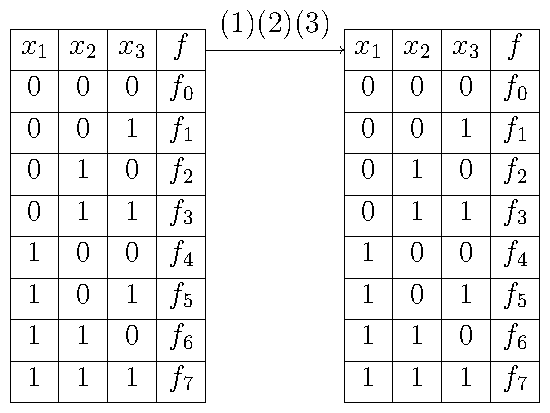
\includegraphics[page=1]{figures/burnside.pdf}
    \caption{Hoán vị $(1)(2)(3)$}
    \label{burnside:first}
\end{figure}

Ta thấy rằng $f_0 \to f_0$, $f_1 \to f_1$, ..., $f_7 \to f_7$ nên có 8 chu trình. Vậy số lượng cách chọn là $2^8$.

Tiếp theo, xét các hoán vị dạng $(1)(2, 3)$, ta có bảng chuyển vector như hình \ref{burnside:second}.

\begin{figure}[ht]
    \centering
    \includegraphics[page=2]{figures/burnside.pdf}
    \caption{Hoán vị $(1)(2, 3)$}
    \label{burnside:second}
\end{figure}

Ta thấy rằng $f_0 \to f_0$, $f_1 \to f_2 \to f_1$, $f_3 \to f_3$, $f_4 \to f_4$, $f_5 \to f_6 \to f_5$, $f_7 \to f_7$. Ở đây có 6 chu trình nên số cách chọn là $2^6$.

Tiếp theo ta xét các hoán vị dạng $(1, 2, 3)$ (hình \ref{burnside:third}).

\begin{figure}[ht]
    \centering
    \includegraphics[page=3]{figures/burnside.pdf}
    \caption{Hoán vị $(1, 2, 3)$}
    \label{burnside:third}
\end{figure}

Ta thấy rằng $f_0 \to f_0$, $f_1 \to f_2 \to f_4 \to f_1$, $f_3 \to f_6 \to f_5 \to f_3$, $f_7 \to f_7$ nên ở đây có 4 chu trình. Số cách chọn là $2^4$.

Như vậy theo bổ đề Burnside, số lớp hàm bool tương đương dưới tác động của nhóm $\mathcal{S}_3$ là \[ t (\mathcal{S}_3) = \dfrac{1}{6}(2^8 + 3 \cdot 2^6 + 2 \cdot 2^4) = 80. \]


\chapter{Giải tích}

\begin{definition}[Dãy Cauchy]
    Dãy $(x_n)$ được gọi là dãy Cauchy nếu với mọi $\varepsilon > 0$, tồn tại $N_0 \in \NN$ sao cho, với mọi $m, n > N_0$ thì $\lvert x_m - x_n \rvert < \varepsilon$.
\end{definition}

\begin{theorem}[Tiêu chuẩn Cauchy]
    Dãy số $(x_n)$ có giới hạn hữu hạn khi và chỉ khi nó là dãy Cauchy.
\end{theorem}

\begin{theorem}[Bổ đề Fermat]
    Cho $f$ là một hàm số có đạo hàm trên $(a, b)$. Nếu $x_0 \in (a, b)$ là một điểm cực trị của $f$ thì ta có $f'(x_0) = 0$.
\end{theorem}

\begin{proof}
    Ta chứng minh trong trường hợp $x_0$ là điểm cực tiểu. Trường hợp điểm cực đại tương tự.

    Hàm $f$ có đạo hàm trên $(a, b)$ nên tại điểm $x_0$ nó có đạo hàm bên trái và đạo hàm bên phải, và hai đạo hàm này bằng nhau.

    Ta có $\displaystyle{f'(x_0^+) = \lim_{x \to x_0^+} \frac{f(x) - f(x_0)}{x - x_0}}$. Vì $x \to x_0^+$ nghĩa là $x > x_0$ ($x$ tiến tới $x_0$ từ bên phải), và do $x_0$ là cực tiểu $f(x) - f(x_0) \geqslant 0$ nên phân số dưới dấu giới hạn lớn hơn 0. Suy ra $f'(x_0^+) \geqslant 0$.

    Hoàn toàn tương tự ta chứng minh được $f'(x_0^-) \leqslant 0$. Và do $f'(x_0^+) = f'(x_0^-) = f'(x_0)$ nên $f'(x_0) = 0$.

    Ta có điều phải chứng minh.
\end{proof}

\begin{theorem}[Định lí Rolle]
    Xét hàm số $f$ liên tục trên đoạn $[a, b]$, có đạo hàm trên khoảng $(a, b)$ và $f(a) = f(b)$. Khi đó tồn tại $c$ thuộc $(a, b)$ sao cho $f'(c) = 0$.
\end{theorem}

\begin{theorem}[Định lí Lagrange]
    Xét hàm số $f$ liên tục trên đoạn $[a, b]$, có đạo hàm trên khoảng $(a, b)$. Khi đó tồn tại $c$ thuộc $(a, b)$ sao cho $f'(c) (b - a) = f(b) - f(a)$.
\end{theorem}

\begin{definition}[Hàm lõm]
    Hàm số $f$ liên tục trên khoảng $\II$ nếu với mọi $\alpha, \beta$ mà $\alpha + \beta = 1$ ta đều có 
    \begin{equation}
        f(\alpha x + \beta y) \leqslant \alpha f(x) + \beta f(y), \quad \forall x, y \in \II
    \end{equation}
\end{definition}

\chapter{Quantum computing}

\section{Qubit và toán tử quantum}

Trên máy tính hiện nay, đơn vị xử lý cơ bản là bit (0 hoặc 1). Trong máy tính lượng tử, đơn vị tính toán là qubit (quantum bit).

\subsection*{Qubit}

Mỗi qubit $\lvert \psi \rangle$ được biểu diễn dưới dạng tổ hợp tuyến tính của cơ sở gồm $\lvert 0 \rangle = (1, 0)$ và $\lvert 1 \rangle = (0, 1)$. Khi đó qubit $\lvert \psi \rangle = \alpha \lvert 0 \rangle + \beta \lvert 1 \rangle$. Ở đây $\alpha, \beta \in \mathbb{C}$ (tập số phức).

Tích của $n$ qubit là các tổ hợp $\lvert 0, 0, \ldots, 0 \rangle$, $\lvert 0, 0, \ldots, 1 \rangle$, ..., $\lvert 1, 1, \ldots, 1 \rangle$. Ta cũng ký hiệu $\lvert 0 \rangle \otimes \lvert 1 \rangle = \lvert 01 \rangle$. 

\begin{example}
    Nếu $\lvert \psi \rangle = \alpha \lvert 0 \rangle + \beta \lvert 1 \rangle$ và $\lvert \Psi \rangle = \gamma \lvert 0 \rangle + \delta \lvert 1 \rangle$ thì
    \begin{equation*}
        \lvert \psi \rangle \otimes \lvert \Psi \rangle = (\alpha \lvert 0 \rangle + \beta \lvert 1 \rangle) \otimes (\gamma \lvert 0 \rangle + \delta \lvert 1 \rangle) = \alpha \gamma \lvert 00 \rangle + \alpha \delta \lvert 0 1 \rangle + \beta \gamma \lvert 10 \rangle + \beta \delta \lvert 11 \rangle
    \end{equation*}
\end{example}

Tiếp theo là \textbf{toán tử quantum} và tương ứng với nó là các cổng (gate) trên mạch.

Toán tử quantum tác động lên một qubit hoặc tích của nhiều qubit.

Qubit có dạng $\lvert \psi \rangle = a \lvert 0 \rangle + b \lvert 1 \rangle$. Ta có thể viết hệ số dưới dạng vector cột $\begin{pmatrix} a \\ b \end{pmatrix}$. Khi đó, toán tử quantum sẽ là một ma trận $2 \times 2$ biến đổi vector trên thành vector mới $\begin{pmatrix} c \\ d \end{pmatrix}$ tương ứng với qubit $\lvert \Psi \rangle = c \lvert 0 \rangle + d \lvert 1 \rangle$.

Nói cách khác, đặt toán tử quantum là ma trận $\mathcal{U} = \begin{pmatrix} c_{11} & c_{12} \\ c_{21} & c_{22} \end{pmatrix}$ thì ta có
\begin{equation*}
    \lvert \psi \rangle \to \lvert \Psi \rangle = \mathcal{U} \lvert \psi \rangle, \quad \begin{pmatrix} c_{11} & c_{12} \\ c_{21} & c_{22} \end{pmatrix} \cdot \begin{pmatrix} a \\ b \end{pmatrix} = \begin{pmatrix} c \\ d \end{pmatrix}
\end{equation*}

\subsection*{Các toán tử quantum thường gặp}

\begin{definition}[Toán tử đồng nhất]
    Toán tử đồng nhất identity giữ nguyên qubit đầu vào. Ma trận tương ứng là ma trận đơn vị $I = \begin{pmatrix} 1 & 0 \\ 0 & 1 \end{pmatrix}$.
\end{definition}

\begin{definition}[Toán tử NOT]
    Toán tử NOT có ma trận tương ứng là $\text{NOT} = \begin{pmatrix} 0 & 1 \\ 1 & 0 \end{pmatrix}$. Khi đó $\text{NOT} \lvert \psi \rangle = b \lvert 0 \rangle + a \lvert 1 \rangle$ với $x \in \{ 0, 1 \}$.
\end{definition}

Khi qubit là $\lvert 0 \rangle$ hoặc $\lvert 1 \rangle$, tác dụng của toán tử NOT là phép XOR nên ta có $\text{NOT} \lvert x \rangle = \lvert x \oplus 1 \rangle$.

\begin{definition}[Toán tử Hadamard]
    Ma trận của toán tử Hadamard là $H = \dfrac{1}{\sqrt{2}} \begin{pmatrix} 1 & 1 \\ 1 & - 1 \end{pmatrix}$. 
\end{definition}

\begin{example}
    Xét qubit $\lvert \psi \rangle = a \lvert 0 \rangle + b \lvert 1 \rangle$, toán tử Hadamard tương ứng với phép nhân ma trận
    \begin{equation*}
        \dfrac{1}{\sqrt{2}} \begin{pmatrix} 1 & 1 \\ 1 & - 1 \end{pmatrix} \cdot \begin{pmatrix} a \\ b \end{pmatrix} = \begin{pmatrix} \dfrac{1}{\sqrt{2}} (a + b) \\ \dfrac{1}{\sqrt{2}} (a - b) \end{pmatrix}
    \end{equation*}

    Ta chuyển cột kết quả về lại dạng tổ hợp tuyến tính thì cổng Hadamard hoạt động trên qubit $\lvert \psi \rangle = a \lvert 0 \rangle + b \lvert 1 \rangle$ cho kết quả là
    \begin{equation*}
        H \lvert \psi \rangle = H(a \lvert 0 \rangle + b \lvert 1 \rangle) = \dfrac{1}{\sqrt{2}} (a + b) \lvert 0 \rangle + \dfrac{1}{\sqrt{2}} (a - b) \lvert 1 \rangle
    \end{equation*}
\end{example}

Nếu $\lvert \psi \rangle \equiv \lvert 0 \rangle$ thì tương đương với $a = 1, b = 0$. Ta có $H \lvert 0 \rangle = \dfrac{\lvert 0 \rangle + \lvert 1 \rangle}{\sqrt{2}}$.

Nếu $\lvert \psi \rangle \equiv \lvert 1 \rangle$ thì tương đương với $a = 0, b = 1$. Ta có $H \lvert 1 \rangle = \dfrac{\lvert 0 \rangle - \lvert 1 \rangle}{\sqrt{2}}$.

Tổng quát ta nhận thấy, với $x \in \{ 0, 1 \}$ thì $H \lvert x \rangle = \dfrac{\lvert 0 \rangle + (-1)^x \lvert 1 \rangle}{\sqrt{2}}$.

Ta thấy rằng toán tử ngược của toán tử Hadamard là chính nó.

Tiếp theo là toán tử thường được dùng nhất khi tính toán trên tích của nhiều qubit: toán tử control.

Như đã xem xét ở trên, tích của $n$ qubit sẽ có $2^n$ phần tử tương ứng các bộ $\lvert 0, 0, \ldots, 0, 0 \rangle$, $\lvert 0, 0, \ldots, 0, 1 \rangle$, ... Do đó toán tử control sẽ là ma trận kích thước $2^n \times 2^n$.


\begin{definition}[Toán tử control]    
    Gọi $\mathcal{U} = \begin{pmatrix} c_{11} & c_{12} \\ c_{21} & c_{22} \end{pmatrix}$ là toán tử tác động lên một qubit (ví dụ như 3 toán tử đã đề cập). Xét hai qubit là $\lvert x \rangle = a \lvert 0 \rangle + b \lvert 1 \rangle$ và $\lvert y \rangle = c \lvert 0 \rangle + d \lvert 1 \rangle$. Từ phía trên
    \begin{equation*}
        \lvert x \rangle \otimes \lvert y \rangle = ac \lvert 00 \rangle + ad \lvert 01 \rangle + bc \lvert 10 \rangle + bd \lvert 11 \rangle
    \end{equation*}

    Khi đó toán tử control có dạng ma trận là
    \begin{equation*}
        c \mathcal{U} = \begin{pmatrix} 1 & 0 & 0 & 0 \\ 0 & 1 & 0 & 0 \\ 0 & 0 & c_{11} & c_{12} \\ 0 & 0 & c_{21} & c_{22} \end{pmatrix}
    \end{equation*}

    Hay viết dưới dạng ma trận khối là $c \mathcal{U} = \begin{pmatrix} I & \mathcal{O} \\ \mathcal{O} & \mathcal{U} \end{pmatrix}$.
\end{definition}

Ta cũng viết tích $\lvert x \rangle \otimes \lvert y \rangle$ dưới dạng vector cột (4 phần tử). Khi đó
\begin{equation*}
    \mathcal{U} (\lvert x \rangle \otimes \lvert y \rangle) = \begin{pmatrix} 1 & 0 & 0 & 0 \\ 0 & 1 & 0 & 0 \\ 0 & 0 & c_{11} & c_{12} \\ 0 & 0 & c_{21} & c_{22} \end{pmatrix} \cdot \begin{pmatrix} ac \\ ad \\ bc \\ bd \end{pmatrix} = \begin{pmatrix} ac \\ ad \\ c_{11} \cdot bc + c_{12} \cdot bd \\ c_{21} \cdot bc + c_{22} \cdot bd \end{pmatrix}
\end{equation*}

Hai phần tử đầu của vector kết quả không thay đổi, còn phần sau có "một phần" là $\mathcal{U} \lvert y \rangle$. Khi viết lại kết quả dưới dạng qubit thì
\begin{equation*}
    ac \lvert 00 \rangle + ad \lvert 01 \rangle + (c_{11} \cdot bc + c_{12} \cdot bd) \lvert 10 \rangle + (c_{21} \cdot bc + c_{22} \cdot bd) \lvert 11 \rangle
\end{equation*}

Ta có một số nhận xét sau đây.

Nếu $\lvert x \rangle \equiv \lvert 0 \rangle$, tức là $a = 1, b = 0$ thì tích trên tương ứng với $c \lvert 00 \rangle + d \lvert 01 \rangle + 0 \lvert 10 \rangle + 0 \lvert 11 \rangle = \lvert 0 \rangle \otimes (c \lvert 0 \rangle + d \lvert 1 \rangle) = \lvert x \rangle \otimes \lvert y \rangle$.

Nếu $\lvert x \rangle \equiv \lvert 1 \rangle$, tức là $a = 0, b = 1$ thì tích trên tương ứng với $0 \lvert 00 \rangle + 0 \lvert 01 \rangle + (c_{11} c + c_{12} d) \lvert 10 \rangle + (c_{21} c + c_{22} d) \lvert 11 \rangle = \lvert 1 \rangle \otimes ((c_{11} c + c_{12} d) \lvert 0 \rangle + (c_{21} c + c_{22} d) \lvert 1 \rangle) = \lvert 1 \rangle \otimes \mathcal{U} \lvert y \rangle = \lvert x \rangle \otimes \mathcal{U} \lvert y \rangle$.

Tổng kết lại, với $x \in \{ 0, 1\}$ thì

\begin{itemize}
    \item nếu $x = 0$ thì $\lvert x \rangle \otimes \lvert y \rangle \to \lvert x \rangle \otimes \lvert y \rangle$.
    \item nếu $x = 1$ thì $\lvert x \rangle \otimes \lvert y \rangle \to \lvert x \rangle \otimes \mathcal{U} \lvert y \rangle$.
\end{itemize}

Tùy vào $x$ là 0 hay 1 mà toán tử quantum $\mathcal{U}$ sẽ bị bỏ qua hoặc xem xét. Ở đây qubit $\lvert x \rangle$ đóng vai trò điều khiển nên đây được gọi là toán tử control.

\begin{definition}[Toán tử control CNOT (Control NOT)]
    Toán tử quantum CNOT có ma trận là
    \begin{equation*}
        \begin{pmatrix} 1 & 0 & 0 & 0 \\ 0 & 1 & 0 & 0 \\ 0 & 0 & 0 & 1 \\ 0 & 0 & 1 & 0 \end{pmatrix} = \begin{pmatrix} I & \mathcal{O} \\ \mathcal{O} & \text{NOT} \end{pmatrix}
    \end{equation*}
\end{definition}

Qubit $\lvert x \rangle$ với $x \in \{ 0, 1 \}$ đóng vai trò control cho qubit $\lvert y \rangle$. Khi $x \equiv 0$ thì $y$ giữ nguyên, hay $\lvert y \oplus 0 \rangle = \lvert y \oplus x \rangle$. Khi $x \equiv 1$ thì áp dụng cổng NOT bên trên, khi đó $y$ biến đổi thành $y \oplus 1 = y \oplus x$.

\chapter{Lý thuyết xác suất}

\section{Định nghĩa xác suất}

\begin{definition}[Định nghĩa cổ điển của xác suất]
    Định nghĩa thống kê của xác suất nói rằng, giả sử trong một phép thử có $n$ khả năng có thể xảy ra. Xét một biến cố $A$ xảy ra khi thực hiện phép thử có $k$ khả năng xảy ra. Khi đó xác suất của biến cố $A$ ký hiệu là $P(A)$ và được tính \[P(A) = \frac{k}{n}\]
\end{definition}

Dễ thấy, do biến cố $A$ là một trường hợp nhỏ trong tổng thể tất cả trường hợp khi thực hiện phép thử, do đó $0 \leq k \leq n$. Nghĩa là \[0 \leq P(A) \leq 1\] với mọi biến cố $A$ bất kì.

\begin{example}
    Xét phép thử tung hai đồng xu. Gọi $A$ là biến cố hai đồng xu cùng mặt.
    
    Ta ký hiệu $S$ là đồng xu sấp, $N$ là đồng xu ngửa. Khi đó các trường hợp có thể xảy ra của phép thử là $S-S$, $S-N$, $N-S$, $N-N$ (4 trường hợp). 
    
    Trong khi đó, các trường hợp có thể xảy ra của biến cố $A$ là $S-S$, $N-N$ (2 trường hợp).
    
    Kết luận: $P(A) = \frac{2}{4} = \frac{1}{2}$
\end{example}

Chúng ta gọi tập hợp tất cả các trường hợp khi thực hiện phép thử là \textbf{không gian mẫu} và ký hiệu là $\Omega$. Mỗi phần tử trong không gian mẫu được gọi là \textbf{biến cố sơ cấp}. Trong ví dụ trên, $\Omega = \{S-S, S-N, N-S, N-N\}$.
    
Tập hợp các trường hợp có thể xảy ra của biến cố gọi là \textbf{không gian biến cố} và ký hiệu là $\Omega_A$. Trong ví dụ trên, $\Omega_A = \{S-S, N-N\}$.
    
Như vậy, $P(A) = \frac{|\Omega_A|}{|\Omega|}$

\begin{example}
    Tung hai con súc sắc cân đối và đồng chất. Tính xác suất tổng số nút của hai con súc sắc bằng 4.
    
    Việc tung mỗi con súc sắc có 6 trường hợp. Do đó $|\Omega| = 6^2 = 36$
    
    Gọi $A$ là biến cố tổng số nút của hai con súc sắc bằng 4. Ta có các trường hợp là $4=1+3=3+1=2+2$ (3 trường hợp).
    
    Như vậy $|\Omega_A| = 3$ và $P(A) = \frac{3}{36} = \frac{1}{12}$
\end{example}

\begin{definition}[Biến cố xung khắc]
    Hai biến cố được gọi là \textbf{xung khắc} nếu biến cố này xảy ra thì biến cố kia chắc chắn không xảy ra. Nói cách khác giao của chúng bằng rỗng.
\end{definition}
    
Khi đó, nếu $A$ và $B$ là hai biến cố xung khắc, \[P(A + B) = P(A) + P(B)\]
    
Ta còn có thể ký hiệu $P(A+B)$ là $P(A \cup B)$ (hợp hai biến cố).
    
\begin{definition}[Biến cố độc lập]
    Hai biến cố được gọi là \textbf{độc lập} nếu việc xảy ra của biến cố này không ảnh hưởng đến việc xảy ra của biến cố kia. 
\end{definition}

Khi đó, nếu $A$ và $B$ là hai biến cố độc lập thì \[P(AB) = P(A)P(B)\]    

\section{Xác suất có điều kiện}

Xét hai tập hợp $A$ và $B$. Số phần tử của phép hợp hai tập hợp trong trường hợp tổng quát được tính như sau: \[|A \cup B| = |A| + |B| - |A \cap B|\]
    
Tương tự, xác suất của phép cộng xác suất đối với hai biến cố có giao khác rỗng là: \[P(A + B) = P(A) + P(B) - P(A \cap B)\]

Xét các tập hợp $A_1$, $A_2$, ..., $A_n$. Khi đó, số phần tử khi hợp các tập hợp này là:
\begin{equation*}
    \begin{split}
        |A_1 \cup A_2 \cup \cdots \cup A_n| & = |A_1| + |A_2| + \cdots + |A_n| - \sum_{i, j}|A_i \cap A_j| \\ & + \sum_{i, j, k} |A_i \cap A_j \cap A_k| + \cdots \\ & = \sum_{i=1}^n (-1)^{i+1} \sum_{j_1, j_2, \cdots, j_i} |A_{j_1} \cap A_{j_2} \cap \cdots \cap A_{j_i} |
    \end{split}
\end{equation*}

Tương tự, ta có phép cộng xác suất:

\begin{theorem}[Phép cộng xác suất mở rộng]
    \begin{equation*}
        P(A_1 \cup A_2 \cup \cdots \cup A_n) = \sum_{i=1}^n (-1)^{i+1} \sum_{j_1, j_2, \cdots, j_i} P(A_{j_1} \cap A_{j_2} \cap \cdots \cap A_{j_i})
    \end{equation*}
\end{theorem}

\begin{theorem}[Xác suất có điều kiện]
    Xét hai biến cố $A$ và $B$. Khi đó xác suất xảy ra của biến cố $B$ với điều kiện biến cố $A$ xảy ra là: 
    \begin{equation}
        P(B | A) = \frac{P(AB)}{P(A)}
    \end{equation}
    Lúc này, $A$ và $B$ không độc lập.
\end{theorem}

Tổng quát, nếu $n$ biến cố $A_i$, $i=1, \ldots, n$ không độc lập thì:
\begin{align*}
    P(A_1 A_2 \cdots A_n) = & P(A_1) \cdot P(A_2|A_1) \cdot P(A_3 | A_2A_1) \cdots \\ & P(A_n|A_1A_2 \cdots A_{n-1})
\end{align*}

\begin{example}
    Xét hai câu hỏi trắc nghiệm có 4 lựa chọn. Tính xác suất học sinh trả lời đúng câu thứ hai với điều kiện câu đầu trả lời sai.
    
    \textbf{Giải}. Gọi $A$ là biến cố câu đầu tiên học sinh trả lời sai. $P(A) = \frac{3}{4}$
    
    Gọi $B$ là biến cố câu thứ hai học sinh trả lời đúng. $P(B) = \frac{1}{4}$.
    
    Do $A$ và $B$ là hai biến cố độc lập nên $P(AB) = P(A) P(B) = \frac{3}{16}$
    
    Như vậy, xác suất học sinh trả lời đúng câu thứ hai với điều kiện câu đầu trả lời đúng là: $P(B | A) = \frac{P(AB)}{P(A)} = \frac{3 / 16}{3 / 4} = \frac{1}{4}$
\end{example}

\section{Công thức xác suất đầy đủ}

\begin{definition}[Hệ biến cố đầy đủ]
    Xét phép thử có không gian mẫu là $\Omega$. Một hệ các biến cố $A_1$, $A_2$, ..., $A_n$ được gọi là \textbf{đầy đủ} nếu chúng thỏa các điều kiện:
    \begin{itemize}
        \item $A_1 \cup A_2 \cup \cdots \cup A_n = \Omega$
        \item $A_i \cap A_j = \emptyset$ với mọi $i \neq j$
    \end{itemize}
\end{definition}
    
\begin{theorem}[Công thức xác suất đầy đủ]
    Gọi $A_1, A_2, \ldots, A_n$ là một hệ biến cố đầy đủ. Khi đó, với biến cố $B$ bất kì trong phép thử: 
    
    \begin{equation}    
        P(B) = P(A_1) \cdot P(B | A_1) + \cdots P(A_n) \cdot P(B | A_n)
    \end{equation}
\end{theorem}

\begin{theorem}[Công thức Bayes]
    Xét hệ có $n$ biến cố đầy đủ $\{ A_1, A_2, \ldots, A_n \}$. 
    
    Với biến cố $B$ bất kì thì: \[P(A_i | B) = \frac{P(A_i) P(B | A_i)}{\displaystyle{\sum_{j=1}^n P(A_j) P(B | A_j)}}\] với $1 \leq i \leq n$.
\end{theorem}

\chapter{Biến ngẫu nhiên}

\section{Biến ngẫu nhiên}

Xét phép thử với không gian mẫu $\Omega$. Với mỗi biến cố sơ cấp $\omega \in \Omega$ ta liên kết với một số thực $\xi(\omega) \in \RR$ thì $\xi$ được gọi là \textbf{biến ngẫu nhiên} (BNN).

\begin{definition}[Biến ngẫu nhiên]
    \textbf{Biến ngẫu nhiên} $\xi$ của một phép thử với không gian mẫu $\Omega$ là ánh xạ: 
    \begin{equation*}
        \begin{split}
            \xi = \xi (\omega), \quad \omega \in \Omega
        \end{split}
    \end{equation*}
\end{definition}
    
Giá trị $\xi(\omega)$ được gọi là một giá trị của biến ngẫu nhiên $\xi$.

\begin{itemize}
    \item Nếu $\xi(\Omega)$ là một tập hữu hạn $\{\xi_1, \xi_2, \ldots,\xi_n\}$ hay tập vô hạn đếm được thì $\xi$ được gọi là \textbf{biến ngẫu nhiên rời rạc}.
    \item Nếu $\xi(\Omega)$ là một khoảng của $\RR$ hay toàn bộ $\RR$ thì $\xi$ được gọi là \textbf{biến ngẫu nhiên liên tục}.
\end{itemize}

\begin{definition}[Hàm phân phối]
    \textbf{Hàm phân phối} của biến ngẫu nhiên $\xi$ là hàm số $F(x)$, xác định bởi:
    \begin{equation}
        F(x) = P(\xi \leq x), \quad x \in \RR
    \end{equation}
\end{definition}

Ở đây ta viết gọn $P(\xi \leq x)$ từ $P(\{ \omega: \xi(\omega) \leq x \})$. Tập hợp $\{ \omega: \xi(\omega) \leq x\}$ có thể không thuộc một biến cố nào, do đó có thể là tập rỗng (ứng với xác suất là 0).
\section{Tính chất của hàm phân phối}

\textbf{Tính chất 1.} Hàm phân phối $F(x)$ không giảm trên mọi đoạn thẳng.

\begin{proof}
    Đặt $x_2 > x_1$. Ta thấy rằng \[\{ \xi \leq x_2 \} = \{ \xi \leq x_1 \} + \{ x_1 < \xi \leq x_2 \},\]
    
    Do đó nếu ta lấy xác suất thì cũng có \[ P(\xi \leq x_2) = P(\xi \leq x_1) + P(x_1 < \xi \leq x_2) \]

    Xác suất luôn không âm, hay $P(x_1 < \xi \leq x_2) \geq 0$, suy ra $P(\xi \leq x_2) \geq P(\xi \leq x_1)$, hay $F(x_2) \geq F(x_1)$.
\end{proof}

\textbf{Tính chất 2.} $\displaystyle{\lim_{x \to -\infty} F(x) = 0}$.

\textbf{Tính chất 3.} $\displaystyle{\lim_{x \to +\infty} F(x) = 1}$.

\textbf{Tính chất 4.} Hàm phân phối $F(x)$ liên tục phải trên toàn trục số.

Để chứng minh các tính chất 2, 3, 4 chúng ta cần các tiên đề của sự liên tục (continunity axioms) và sẽ không đề cập ở đây.

\section{Biến ngẫu nhiên rời rạc}

Cho BNN rời rạc $\xi = \xi(\omega)$, $\xi = \{ a_1, a_2, \ldots, a_n, \ldots \}$. Giả sử $a_1 < a_2 < \ldots < a_n < \ldots$ với xác suất tương ứng là $P(\xi = a_i) = p_i$, $i = 1, 2, \ldots$

Ta có thể biểu diễn biến ngẫu nhiên và xác suất tương ứng của nó bằng bảng phân phối xác suất của $\xi$.

\begin{table}[ht]
    \centering
    \begin{tabular}{c|c c c c c}
        $\xi$ & $a_1$ & $a_2$ & $\cdots$ & $a_n$ & $\cdots$ \\ \hline $P$ & $p_1$ & $p_2$ & $\cdots$ & $p_n$ & $\cdots$
    \end{tabular}
\end{table}

Rõ ràng rằng $p_n \geq 0$ với mọi $n$. Hơn nữa \[ \sum_{n=1}^\infty p_n = 1 \]

Không gian mẫu lúc này là hợp của các tập biến ngẫu nhiên rời rạc: \[ \Omega = \{ \xi = a_1 \} \cup \{ \xi = a_2 \} \cup \ldots \]

Các biến ngẫu nhiên xung khắc nhau (vì $\xi$ không thể nhận hai giá trị khác nhau cùng lúc), do đó xác suất cả không gian mẫu là \[ 1 = P(\Omega) = P(\xi = a_1) + P(\xi = a_2) + \ldots = p_1 + p_2 + \ldots \]

\begin{definition}[Phân phối nhị thức]
    Biến ngẫu nhiên $\xi$ được gọi là có \textbf{phân phối nhị thức} với tham số $p$, $n$, với $p \in (0, 1)$ và $n$ là số tự nhiên, nếu $\xi$ nhận các giá trị $0, 1, \ldots, n$ và 
    \begin{equation}
        P(\xi = k) = C^k_n p^k q^{n-k}, \quad k = 0, 1, \ldots, n
    \end{equation}
    Ở đây $q = 1 - p$.
\end{definition}

\begin{example}
    Một bài kiểm tra có 100 câu hỏi trắc nghiệm bốn đáp án. Xác suất chọn ngẫu nhiên đúng đáp án của mỗi câu hỏi thì bằng nhau và bằng $\dfrac{1}{4}$.

    Ở đây xác suất chọn ngẫu nhiên đúng đáp án của một câu hỏi bất kì là $p = \dfrac{1}{4}$, và số lượng câu hỏi là $n = 100$.

    Gọi $\xi$ là biến ngẫu nhiên số câu hỏi trả lời đúng. Khi đó $\xi$ nhận các giá trị $0, 1, \ldots, 100$.

    Do đó bài toán này có phân phối nhị nhức và \[ P(\xi = k) = C^k_{100} \Bigl(\dfrac{1}{4}\Bigr)^k \Bigl(\dfrac{3}{4}\Bigr)^{100-k}\]    
\end{example}

\begin{definition}[Phân phối Poisson]
    Biến ngẫu nhiên $\xi$ được gọi là có \textbf{phân phối Poisson} với tham số $\lambda$, nếu $\xi$ nhận các giá trị $0, 1, \ldots, n$ và 
    \begin{equation}
        P(\xi = k) = \dfrac{\lambda^k \cdot e^{-\lambda}}{k!}, \quad k = 0, 1, \ldots, n
    \end{equation}
\end{definition}

Tham số $\lambda$ thể hiện số lần trung bình mà một sự kiện xảy ra trong một khoảng thời gian nhất định. Khi đó, nếu một biến ngẫu nhiên có số lần xuất hiện trung bình của một sự kiện trong thời gian $t$ thì nó có phân phối Poisson với tham số $\lambda t$, với $\lambda$ là số lần trung bình trong một đơn vị thời gian.

\section{Biến ngẫu nhiên liên tục}

\begin{definition}[Biến ngẫu nhiên liên tục]
    Biến ngẫu nhiên $\xi$ được gọi là \textbf{liên tục}, nếu nó nhận giá trị tại mọi điểm thuộc một đoạn liên tục nào đó trên trục số, và tồn tại một hàm số không âm $p(x)$ sao cho với mọi đoạn $[a ,b]$ (hữu hạn hoặc vô hạn) ta có
    \begin{equation}
        P(a \leq \xi \leq b) = \int_{a}^{b} p(x)\, dx
    \end{equation}
    Hàm $p(x)$ được gọi là \textbf{hàm mật độ} của biến ngẫu nhiên $\xi$.
\end{definition}

Tương tự biến ngẫu nhiên rời rạc, $p(x) \geq 0$ với mọi $x \in \RR$ và khi hai cận là vô cực thì biến ngẫu nhiên bao quát toàn bộ không gian mẫu. Nghĩa là \[ \int_{-\infty}^{+\infty} p(x)\, dx = 1 \]

Từ định nghĩa của hàm phân phối $F(x) = P(\xi \leq x)$ ta có hai tính chất của hàm mật độ:

\begin{enumerate}
    \item $\displaystyle{F(x) = \int_{-\infty}^{x} p(x)\, dx}$
    \item $p(x) = F'(x)$
\end{enumerate}

Tính chất thứ nhất là từ định nghĩa hàm phân phối. Tính chất thứ hai suy ra từ việc cận trên của tích phân là hữu hạn.

\textbf{Hàm mật độ của $X$ là} \[f(x) = \begin{cases}
        p_i & \text{khi } x = x_i, \\
        0 & \text{khi } x \neq x_i, \forall i
\end{cases}\]

\begin{remark}
    Ta có các lưu ý sau:
    \begin{itemize}
        \item $p_i \geq 0$, $\sum p_i = 1$, $i = 1, 2, \ldots$
    
        \item $\displaystyle{P(a < X \leq b) = \sum_{a < x_i \leq b} p_i}$
    \end{itemize}
\end{remark}

\section{Hàm mật độ của biến ngẫu nhiên liên tục}

\begin{definition}
    Hàm số $f: \mathbb{R} \mapsto \mathbb{R}$ được gọi là \textbf{hàm mật độ} của biến ngẫu nhiên liên tục $X$ nếu: \[P(a \leq X \leq b) = \displaystyle{\int_a^b f(x)\,dx}, \forall a, b \in \mathbb{R}\]
\end{definition}

\begin{remark}
    Với mọi $x \in \mathbb{R}$, $f(x) \geq 0$ và $\displaystyle{\int_{-\infty}^{+\infty}f(x)\,dx = 1}$.
\end{remark}

\textbf{Ý nghĩa hình học}. Xác suất của biến ngẫu nhiên $X$ nhận giá trị trong $[a, b]$ bằng diện tích hình thang cong giới hạn bởi $x=a$, $x=b$, $y=f(x)$ và $Ox$.


\chapter{Hình học giải tích}

\section{Theo dòng lịch sử}

Hình học xuất hiện từ thời xa xưa, xuất phát từ những nhu cầu thực tế nhất của con người là đo đạc để phân chia đất đai, xây dựng, canh tác, ... Từ đó con người đã có nhận thức rất sớm về quan hệ song song và vuông góc giữa hai đường thẳng.

Một cách hình ảnh (mà thật ra hình học là môn học về hình ảnh) thì hai đường thẳng song song không cắt nhau dù có kéo dài chúng ra vô tận. Các đường thẳng song song luôn có nhiều điều thú vị, cả ở mặt phẳng Euclid lẫn trong không gian. Đầu tiên phải kể đến định lý mang tên triết gia vĩ đại của Hy Lạp: Thales.

\subsection*{Thales của Miletus}

Thales của Miletus được cho rằng sinh vào khoảng năm 624 Trước Công nguyên (TCN) và mất năm 547 TCN tại Miletus (Thổ Nhĩ Kì ngày nay)\footnote{\url{https://mathshistory.st-andrews.ac.uk/Biographies/Thales/}}.

\begin{figure}[ht]
	\centering
	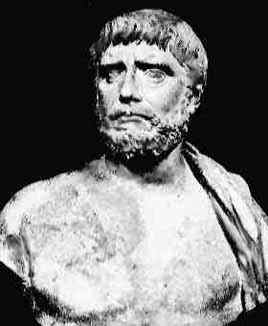
\includegraphics[scale=0.5]{analytic_geometry/Thales.jpeg}
	\captionsetup{labelformat=empty}
	\caption{Thales của Miletus}
\end{figure}

Ông được xem là nhà triết học đầu tiên khi không cố gắng giải thích tự nhiên bằng thần thoại hay các thế lực siêu nhiên như trước. Trường phái triết học do ông sáng lập, trường phái Milet, cho rằng mọi vật có nguồn gốc từ nước. Nhà triết học nổi tiếng Aristotle đánh giá rằng Thales là người sáng lập ra \textit{triết học duy vật sơ khai}.

Trong toán học, Thales được biết tới với định lý mang tên ông về các đường song song. Định lý Thales được phát biểu như sau:

\begin{theorem}[Định lý Thales]
    Trong một tam giác, đường thẳng song song với một cạnh chắn trên hai cạnh còn lại các đoạn thẳng tương ứng tỉ lệ.
\end{theorem}

\begin{figure}[ht]
	\centering
	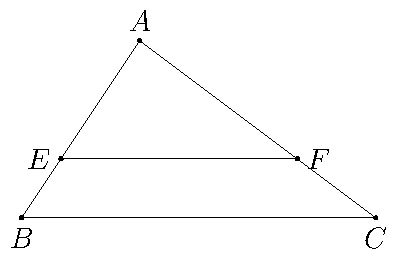
\includegraphics{analytic_geometry/thales1.pdf}
	\caption{Định lý Thales trên mặt phẳng}
	\label{thales1}
\end{figure}

Theo định lý Thales, nếu $EF$ song song với $BC$ thì ta có $\dfrac{AE}{AB} = \dfrac{AF}{AC} = \dfrac{EF}{BC}$ (hình \ref{thales1}).

Không dừng lại ở mặt phẳng, khi mở rộng lên không gian định lý Thales cũng cho chúng ta một kết quả quan trọng khi nói tới các mặt phẳng song song nhau.

\begin{theorem}[Định lý Thales trong không gian]
    Trong khối chóp, mặt phẳng song song mặt đáy chắn các cạnh nối từ đỉnh hình chóp tới các đỉnh của mặt phẳng đáy các đoạn thẳng tương ứng tỉ lệ.
\end{theorem}

\begin{figure}[ht]
	\centering
	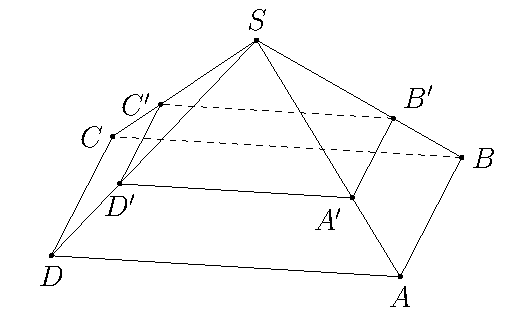
\includegraphics{analytic_geometry/thales2.pdf}
	\caption{Định lý Thales trong không gian}
	\label{thales2}
\end{figure}

Theo định lý Thales, nếu mặt phẳng $(ABCD)$ song song với mặt phẳng $(A'B'C'D')$ thì $\dfrac{SA}{SA'} = \dfrac{SB}{SB'} = \dfrac{SC}{SC'} = \dfrac{SD}{SD'}$ (hình \ref{thales2}).

\subsection*{Pythagoras của Samos}

Khi nhắc tới vuông góc, chúng ta thường nhớ tới định lý ngày nào được học ở thời học sinh: định lý Pythagoras. Định lý này nói về quan hệ giữa độ dài các cạnh trong một tam giác vuông. Định lý tuy đơn giản nhưng có ý nghĩa rất quan trọng trong đời sống và khoa học của con người suốt chiều dài lịch sử. Đây cũng là tiền đề cho định lý mang tính lịch sử của nhân loại: định lý cuối cùng của Fermat.

\begin{figure}[ht]
	\centering
	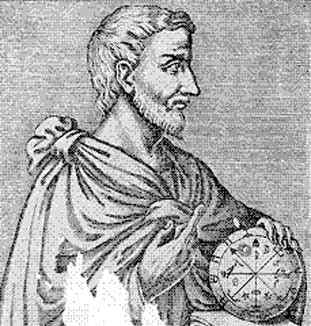
\includegraphics[scale=0.5]{analytic_geometry/Pythagoras.jpeg}
	\captionsetup{labelformat=empty}
	\caption{Pythagoras của Samos}
\end{figure}

Pythagoras của Samos cũng là nhà triết học Hy Lạp cổ, được cho rằng sinh vào khoảng năm 570 TCN và mất năm  490 TCN\footnote{\url{https://mathshistory.st-andrews.ac.uk/Biographies/Pythagoras/}}. Ông được học tập từ nhà triết học Thales và cũng có nhiều đóng góp cho sự phát triển của toán học, thiên văn học và âm nhạc. Tuy nhiên khác với thầy mình, trường phái triết học của ông cho rằng những con số là nguồn gốc của vạn vật và sử dụng những con số để giải thích những hiện tượng khoa học. Từ đây, các lý thuyết về âm nhạc được ra đời, cụ thể là các mối liên hệ về tần số với sự rung của dây nhạc cụ.

Ông là một trong những người hiếm hoi cho phép cả phụ nữ đi học ở lớp của mình vào thời ấy. Điều đó giúp phổ biến toán học nói riêng và kiến thức nói chung tới nhiều tầng lớp nhân dân. Tuy nhiên ông cũng có một hội kín rất thú vị. Như đã nói ở trên, trường phái triết học Pythagoras cố gắng giải thích nguồn gốc vạn vật bằng những con số. Điều này đã dẫn họ tới những khám phá động trời vào thời ấy.

Một trong những khám phá đó là về sự tồn tại của số vô tỉ dựa vào định lý mang tên ông. Lịch sử đã chỉ ra rằng trước Pythagoras, người Babylon và Ai Cập đã tìm ra rất nhiều bộ số nguyên $(a, b, c)$ thỏa mãn $a^2 + b^2 = c^2$ là độ dài ba cạnh tam giác vuông. Định lý Pythagoras mà ngày nay chúng ta biết được phát biểu rằng:

\begin{theorem}[Định lý Pythagoras]
    Trong một tam giác vuông, bình phương độ dài cạnh huyền bằng tổng bình phương độ dài hai cạnh góc vuông.
\end{theorem}

Như vậy nếu gọi độ dài cạnh huyền là $c$, độ dài hai cạnh góc vuông lần lượt là $a$ và $b$ thì $a^2 + b^2 = c^2$ (hình \ref{pythagoras1}).

\begin{figure}[ht]
	\centering
	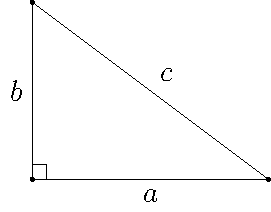
\includegraphics{analytic_geometry/pythagoras1.pdf}
	\caption{Định lý Pythagoras}
	\label{pythagoras1}
\end{figure}

Nếu $a = b = 1$ thì sao? Khi đó bình phương độ dài cạnh huyền $c^2 = 2$. Tuy nhiên không thể tìm ra một số hữu tỉ nào để bình phương lên là 2 cả. Phát hiện này là một chấn động đối với thời Pythagoras và ông yêu cầu tất cả thành viên trong hội phải giữ kín bí mật về sự phát hiện này. Tuy nhiên thông tin vẫn lọt ra ngoài và truyền thuyết kể rằng ông đã xử tội chết cho thành viên của hội không tuân thủ.

Pythagoras đã đưa một khái niệm cực kì quan trọng trong toán học, gọi là \textit{chứng minh} (proof). Để chứng minh một mệnh đề là đúng, chúng ta cần các mệnh đề (thường đơn giản hơn) đúng trước đó. Bằng các phép suy luận thích hợp dựa trên các mệnh đề đúng trước đó, chúng ta có thể kết luận rằng mệnh đề cần chứng minh là đúng. Phép chứng minh có thể gọi là \textit{xương sống} của toán học, vì nếu không có một phép chứng minh đúng đắn thì một mệnh đề không thể được xác định được là có đúng hay không. Trong trường hợp của Fermat, khi ông đưa ra định lý Fermat nhưng không kèm chứng minh (vì lề sách quá chật nên không viết lời giải được) thì chúng ta không thể biết định lý Fermat có đúng hay không (?).

Nếu việc suy luận dựa trên các mệnh đề, hoặc định lý, đã đúng trước đó, thì phải có một lúc nào đó việc này dừng lại. Chúng ta không thể suy ngược tới vô hạn lần được. Do đó chúng ta cần những mệnh đề luôn đúng nhưng tính đúng đắn của nó được kiểm nghiệm trong thực tiễn. Chúng được gọi là \textit{tiên đề} (axiom). Nhân vật tiếp theo được đề cập tới sẽ dẫn chúng ta tới hệ thống tiên đề làm nền tảng cho hình học.

\subsection*{Euclid của Alexandria}

Đúng vậy, Euclid là người đặt nền móng cho hình học với bộ sách nổi tiếng \textit{Elements} của mình. Trong bộ sách này đề cập tới những tiên đề, định lý làm nền tảng cho bộ môn hình học và vẫn còn ý nghĩa cho tới tận ngày nay. Những gì viết trong đó không quá xa lạ với những gì được giảng dạy trong nhà trường.

\begin{figure}[ht]
	\centering
	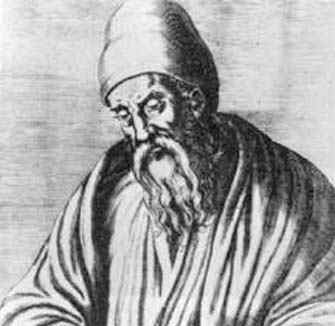
\includegraphics[scale=0.5]{analytic_geometry/Euclid.jpeg}
	\captionsetup{labelformat=empty}
	\caption{Euclid của Alexandria}
\end{figure}

Euclid của Alexandria sinh vào khoảng năm 325 TCN và mất vào khoảng năm 265 TCN\footnote{\url{https://mathshistory.st-andrews.ac.uk/Biographies/Euclid/}}. Thông tin về ông không có nhiều. Nhưng chỉ mỗi bộ sách \textit{Elements} cũng đủ để người đời sau cho rằng ông là người có ảnh hưởng nhất trong 2000 năm lịch sử phát triển của toán học.

Năm tiên đề cơ bản của hình học được ông phát biểu trong bộ \textit{Elements} được phát biểu như sau:

\begin{enumerate}
	\item Qua hai điểm bất kì luôn vẽ được một đường thẳng
	\item Đường thẳng có thể kéo dài vô hạn về cả hai phía
	\item Ta có thể xác định một đường tròn bằng tâm và bán kính của nó
	\item Mọi góc vuông đều bằng nhau
	\item Nếu một đường thẳng cắt hai đường thẳng khiến tổng hai góc trong cùng phía nhỏ hơn hai vuông thì hai đường thẳng đó chắc chắn sẽ cắt nhau tại một điểm nào đó
\end{enumerate}

Tiên đề số 5 là rắc rối và phức tạp nhất. Nó không thực sự tự nhiên và có nhiều sự vướng mắc. Đây chính là tiên đề cho sự ra đời của hình học phi-Euclid hơn 1500 năm sau.

Bộ \textit{Elements} của Euclid bao gồm 13 quyển. Trong đó đề cập tới rất nhiều vấn đề của hình học, từ những phần tử đơn giản nhất cấu tạo nên hình học là điểm, đoạn thẳng, đường thẳng, tới những hình học lớn hơn như hình chữ nhật, hình tròn, đa giác, mặt phẳng. Thậm chí ông cũng đã có những dấu chân ở hình học không gian như hình chóp, hình cầu, hình nón (\cite{Euclid}, \cite{Casey2007}).

\section{Phương pháp tọa độ trong mặt phẳng}

Cuộc cách mạng trong hình học xảy ra khi nhà toán học lãng tử René Descartes phát minh ra hệ tọa độ và từ đó mọi đối tượng hình học có thể được biểu diễn bởi các phương pháp đại số như phương trình, đẳng thức.

\begin{figure}[ht]
	\centering
	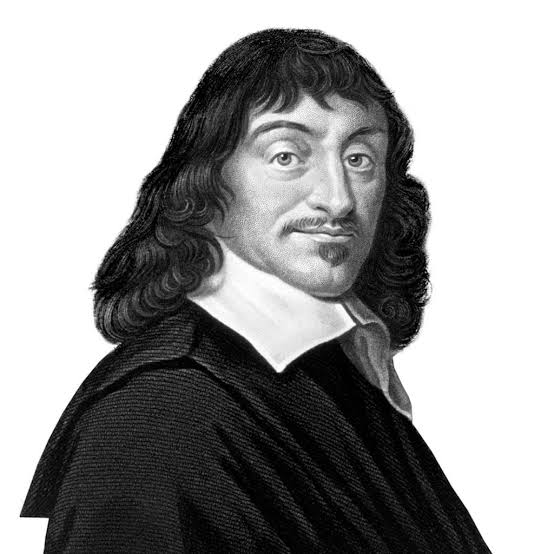
\includegraphics[scale=0.5]{mathematicians/Descartes.jpg}
	\captionsetup{labelformat=empty}
	\caption{René Descartes (1596-1650)}
\end{figure}

\subsection*{Danh mục thuật ngữ và ký hiệu}

Đầu tiên chúng ta thống nhất các thuật ngữ cũng như ký hiệu được sử dụng kể từ đây.

\textbf{Điểm} là đơn vị cơ bản của hình học. Bất kì đối tượng hình học nào cũng là một \textit{tập hợp điểm}. Điểm được ký hiệu bởi chữ in hoa, ví dụ như $A$, $B_1$, $B_2$.

\textbf{Đường thẳng} đi qua hai điểm phân biệt cho trước. Đường thẳng có thể kéo dài vô hạn về hai phía. Đường thẳng được ký hiệu bởi chữ in thường hoặc chữ Hy Lạp trong ngoặc đơn, ví dụ như $(d)$, $(\Delta)$.

\textbf{Đoạn thẳng} chỉ phần đường thẳng nằm giữa hai điểm.

\textbf{Nửa đường thẳng} chỉ phần đường thẳng nằm một phía của một điểm trên đường thẳng và chỉ kéo dài vô hạn về phía đó.

\textbf{Vector} là đoạn thẳng có hướng. Với điểm đầu là $A$ và điểm cuối là $B$ thì vector từ $A$ tới $B$ được ký hiệu là $\overrightarrow{AB}$. Để chỉ một vector không cần biết điểm đầu và điểm cuối ta dùng chữ thường in đậm, ví dụ như $\bm{a}$.

\textbf{Góc giữa hai vector} $\overrightarrow{OA}$ và $\overrightarrow{OB}$ là góc $\angle AOB$ và ký hiệu là $(\overrightarrow{OA}, \overrightarrow{OB})$.

Tương tự đối với vector $\bm{a}$ và $\bm{b}$ thì góc giữa chúng ký hiệu là $(\bm{a}, \bm{b})$.

\subsection*{Vector trong mặt phẳng}

Trong hệ tọa độ $Oxy$ với tâm $O$ và hai trục $Ox$ (trục hoành) và $Oy$ (trục tung) vuông góc nhau, đặt $O = (0, 0)$ là tọa độ của tâm $O$.

Tiếp theo, mọi điểm trong mặt phẳng Euclid đi liền với cặp số $(x, y)$ chỉ tọa độ của điểm đó. Ví dụ $A = (1, 3)$, $B = (4, 1)$.

\begin{figure}[ht]
	\centering
	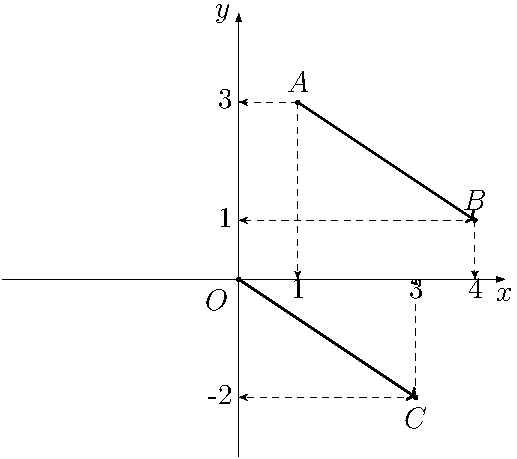
\includegraphics[page=1]{analytic_geometry/oxy1.pdf}
	\caption{Tọa độ của điểm trong mặt phẳng}
	\label{oxy1}
\end{figure}

Tọa độ của điểm cũng là tọa độ của vector từ $O$ tới điểm đó. Với hình \ref{oxy1} thì $\overrightarrow{OA} = (1, 3)$ và $\overrightarrow{OB} = (4, 1)$. Tọa độ của vector $\overrightarrow{AB}$ khi đó sẽ là $\overrightarrow{AB} = \overrightarrow{OB} - \overrightarrow{OA} = (4, 1) - (1, 3) = (3, -2)$. Cũng theo hình \ref{oxy1} thì ta thấy $\overrightarrow{AB} = \overrightarrow{OC} = (3, -2)$. 

Như vậy, nếu ta có hai điểm $A = (x_A, y_A)$ và $B = (x_B, y_B)$ thì vector $\overrightarrow{AB}$ là
\begin{equation}
	\overrightarrow{AB} = (x_B - x_A, y_B - y_A)
\end{equation}

\textbf{Tích vô hướng của hai vector} $\bm{a} = (x_1, y_1)$ và $\bm{b} = (x_2, y_2)$ được định nghĩa là
\begin{equation}
	\langle \bm{a}, \bm{b} \rangle = x_1 x_2 + y_1 y_2
\end{equation}

Ta cũng có thể ký hiệu tích vô hướng là $\bm{a} \cdot \bm{b}$.

Ta ký hiệu $\lVert \bm{a} \rVert$ là độ dài (chuẩn Euclid, Euclid norm) của vector $\bm{a}$. Trong hệ tọa độ Descartes vuông góc, theo định lý Pythagoras, độ dài của vector là độ dài cạnh huyền tam giác vuông (hình \ref{oxy1}). Như vậy, độ dài đoạn thẳng $AB$ với $A = (x_A, y_A)$ và $B = (x_B, y_B)$ là
\begin{equation}
	AB = \lVert \overrightarrow{AB} \rVert = \sqrt{(x_B - x_A)^2 + (y_B - y_A)^2}
\end{equation}

Khi đó cosin góc giữa hai vector $\bm{a}$ và $\bm{b}$ là
\begin{equation}
	\cos (\bm{a}, \bm{b}) = \frac{\bm{a} \cdot \bm{b}}{\lVert \bm{a} \rVert \cdot \lVert \bm{b} \rVert} = \frac{x_1 x_2 + y_1 y_2}{\sqrt{x_1^2 + y_1^2} \cdot \sqrt{x_2^2 + y_2^2}}
\end{equation}

Nếu góc giữa hai vector bằng 90 độ thì hai vector được gọi là vuông góc nhau. Khi đó tích vô hướng $\bm{a} \cdot \bm{b} = 0$.

\subsection*{Phương trình đường thẳng trong mặt phẳng}

Theo tiên đề Euclid, một đường thẳng được xác định khi biết hai điểm phân biệt thuộc đường thẳng đó. Trong hệ tọa độ, chúng ta có hai cách tìm phương trình đường thẳng.

\textbf{Bằng vector pháp tuyến}. Vector pháp tuyến của đường thẳng là vector vuông góc với mọi vector có phương là đường thẳng đó. Giả sử $\bm{v} = (a, b)$ là vector pháp tuyến của đường thẳng đi qua điểm $M_0 = (x_0, y_0)$. Khi đó đường thẳng đi qua qua $M_0$ nhận $\bm{v}$ làm vector pháp tuyến là \textit{tập hợp điểm} $M = (x, y)$ trên mặt phẳng sao cho $\bm{v} \cdot \overrightarrow{M_0 M} = 0$. Điều này tương đương với
\begin{equation}
	\bm{v} \cdot \overrightarrow{M_0 M} = a \cdot (x - x_0) + b \cdot (y - y_0) = 0
\end{equation}

\textbf{Bằng vector chỉ phương}. Vector chỉ phương của đường thẳng là vector có phương song song với đường thẳng đó. Giả sử $\bm{v}' = (a', b')$ là vector chỉ phương của đường thẳng đi qua điểm $M_0 = (x_0, y_0)$. Khi đó đường thẳng đi qua $M_0$ nhận $\bm{v}'$ làm vector chỉ phương là \textit{tập hợp điểm} $M = (x, y)$ trên mặt phẳng sao cho $\bm{v}' \parallel \overrightarrow{M_0 M}$. Điều này tương đương với
\begin{equation}
	\bm{v}' \parallel \overrightarrow{M_0 M} \Leftrightarrow \frac{x - x_0}{a'} = \frac{y - y_0}{b'}
\end{equation}

\begin{enumerate}
	\item Cả hai cách biểu diễn khi khai triển ra đều có dạng $a x + by + c = 0$ với $c$ là hằng số. Đây được gọi là dạng tổng quát của phương trình đường thẳng. 
	
	\item Cách viết $\dfrac{x - x_0}{a'} = \dfrac{y - y_0}{b'}$ được gọi là dạng chính tắc của phương trình đường thẳng.
	
	\item Dạng chính tắc của phương trình đường thẳng còn có một tác dụng đặc biệt khác \[\frac{x - x_0}{a'} = \frac{y - y_0}{b'} = t\] với $t \in \mathbb{R}$. Khi đó tọa độ $M = (x, y)$ có thể được biểu diễn dưới dạng
	\begin{equation}
		\begin{cases}
			x = x_0 + a' t \\ y = y_0 + b' t
		\end{cases}, \quad t \in \mathbb{R}
	\end{equation}
	Đây được gọi là phương trình dạng tham số.
\end{enumerate}

Chúng ta chú ý rằng nếu đường thẳng song song với một trong hai trục tọa độ thì vector chỉ phương của nó sẽ cùng phương với vector đơn vị $(1, 0)$ hoặc $(0, 1)$. Do đó không thể viết dưới dạng chính tắc được (không thể chia cho 0) nhưng có thể viết dưới dạng tổng quát hoặc dạng tham số.

\subsection*{Khoảng cách giữa điểm và đường thẳng}

Nhắc lại một chút kiến thức cơ sở. \textbf{Khoảng cách} từ một điểm $A$ nằm ngoài đường thẳng $(d)$ là độ dài đoạn thẳng $AH$ với $H \in (d)$ sao cho $AH$ nhỏ nhất (hình \ref{oxy2}).

Khi đó $H$ được gọi là \textbf{hình chiếu} của $A$ lên đường thẳng $(d)$ và $AH$ là \textbf{khoảng cách} từ $A$ tới $(d)$. Do $AH$ là đoạn thẳng có độ dài ngắn nhất, điều này xảy ra khi $AH \perp (d)$.

\begin{figure}[ht]
	\centering
	\includegraphics[page=2]{analytic_geometry/oxy1.pdf}
	\caption{Hình chiếu và khoảng cách tới đường thẳng}
	\label{oxy2}
\end{figure}

Như vậy, để tìm hình chiếu của điểm $A$ lên đường thẳng $(d)$, ta dựng đường thẳng đi qua điểm $A$ và vuông góc với $(d)$.

Giả sử phương trình đường thẳng $(d)$ với vector pháp tuyến $\bm{v} = (a, b)$ là $(d): ax + by + c = 0$.

Gọi $(d')$ là đường thẳng đi qua $A = (x_0, y_0)$ và vuông góc với $d$. Do $\bm{v}$ là vector pháp tuyến của $(d)$ nên $\bm{v}$ là vector chỉ phương của $(d')$. Khi đó phương trình dạng tham số của $(d')$ là \[\begin{cases}
	x = x_0 + a t \\ y = y_0 + b t
\end{cases}, t \in \mathbb{R}\]

Gọi $H$ là hình chiếu của $A$ lên $(d)$. Khi đó $H$ là giao điểm của $(d)$ và $(d')$. Vì $H \in (d')$ nên tọa độ của $H$ có dạng $(x_0 + at, y_0 + bt)$ với $t$ nào đó thuộc $\mathbb{R}$. Chúng ta sẽ đi tìm $t$ này.

Vì $H \in (d)$ nên ta thay tọa độ của $H$ vừa tìm được vào phương trình của $(d)$ thu được \[a (x_0 + at) + b (y_0 + bt) + c = 0 \Leftrightarrow t = -\frac{a x_0 + b y_0 + c}{a^2 + b^2}\]
Như vậy là ta đã tìm được $t$ từ đó xác định được tọa độ của $H$.

Từ đây ta tính được khoảng cách từ $A$ tới $(d)$ hay nói cách khác là độ dài đường $AH$. Ta có $A = (x_0, y_0)$ và $H = (x_0 + at, y_0 + bt)$ nên $\overrightarrow{AH} = (at, bt)$. Suy ra
\begin{align*}
	AH = & \lVert \overrightarrow{AH} \rVert = \sqrt{(at)^2 + (bt)^2} = \lvert t \rvert \sqrt{a^2 + b^2} \\ = & \Big| -\frac{a x_0 + b y_0 + c}{a^2 + b^2} \Big| \cdot \sqrt{a^2 + b^2} = \frac{\lvert a x_0 + b y_0 + c \rvert}{\sqrt{a^2 + b^2}}
\end{align*}

\section{Đạo hàm}

Phép tính vi tích phân đã được con người nghiên cứu từ lâu. Câu chuyện về ai là người phát minh ra phép tính vi tích phân: Newton hay Leibniz, được coi là một trong những vụ tranh cãi đáng xấu hổ nhất lịch sử toán học. Nhưng họ cũng đã để lại một mảnh đất màu mỡ cho toán học về sau.

\subsection*{Cơ học và sự ra đời của đạo hàm}

Trường phái Newton sử dụng đạo hàm như công cụ khảo sát vận tốc từ quãng đường. Ở bậc trung học chúng ta biết rằng \textit{vận tốc trung bình} bằng quãng đường chia thời gian. Tuy nhiên điều đó chỉ đúng cho \textit{chuyển động thẳng đều}. Nếu quãng đường là một hàm số phụ thuộc thời gian (quãng đường là $s(t)$ với $t$ là thời gian) thì điều đó không đúng nữa.

Do quãng đường phụ thuộc thời gian nên có thể là vận tốc cũng phụ thuộc thời gian? Hợp lí đấy. Nhưng với mỗi một giá trị thời gian $t$ cho ta một vị trí $s(t)$ trên trục số, còn vận tốc thì không thể phụ thuộc một giá trị thời gian được. Rõ ràng vật phải di chuyển một quãng đường từ thời gian $t_0$ tới $t_1$ thì mới có vận tốc trên quãng đường đó chứ?

Cách tiếp cận ở đây là, chúng ta cho sự thay đổi thời gian, tức hiệu $\Delta t = t_1 - t_0$, rất nhỏ. Khi đó vật đi từ $s(t_0)$ tới $s(t_1)$, vậy là chúng ta có thể tính vận tốc với công thức $v = \dfrac{s(t_1) - s(t_0)}{t_1 - t_0}$. Do $\Delta t$ rất nhỏ, hay \textit{tiến về 0}, thì vận tốc gần như xảy ra vào đúng một thời điểm. Do đó vận tốc lúc này được gọi là \textit{vận tốc tức thời}. Đó cũng chính là ý nghĩa cơ học và sự ra đời của đạo hàm theo trường phái Newton.

\subsection*{Định nghĩa đạo hàm}

Xét hàm số $f(x)$ liên tục trên khoảng $(a, b)$ có chứa điểm $x_0$. Đạo hàm của $f(x)$ tại $x_0$ được định nghĩa là giới hạn
\begin{equation}
	f'(x_0) = \lim_{x \to x_0} \frac{f(x) - f(x_0)}{x - x_0}
	\label{der1}
\end{equation}

Lưu ý rằng nếu giới hạn trên không phải là giới hạn hữu hạn (không tồn tại hoặc tiến tới vô cực) thì hàm số không có đạo hàm tại điểm $x_0$.

Ví dụ, để tính đạo hàm của hàm số $f(x) = x^3 + 2 x^2 - 4$ tại $x_0 = 4$, ta khai triển
\begin{align*}
	\frac{f(x) - f(x_0)}{x - x_0} = & \frac{f(x) - f(4)}{x - 4} \\ = & \frac{x^3 + 2x^2 - 4 - (4^3 + 2 \cdot 4^2 - 4)}{x - 4} \\ = & \frac{(x^3 - 4^3) + 2(x^2 - 4^2)}{x - 4} \\ = & \frac{(x-4)(x^2 + 4x + 16) + 2 (x-4)(x+4)}{x - 4} \\ = & x^2 + 4 x + 16 + 2(x+4)
\end{align*}

Cho $x$ tiến tới 4 thì ta có đạo hàm tại $x = 4$
\begin{align*}
	f'(4) = & \lim_{x \to 4} \frac{f(x) - f(4)}{x - 4} \\ = & \lim_{x \to 4} (x^2 + 4x + 16 + 2(x+4)) \\ = & 4^2 + 4 \cdot 4 + 16 + 2 \cdot (4 + 4) = 64
\end{align*}

Trong định nghĩa ở \ref{der1}, nếu ta đặt $\Delta x = x - x_0$ và $\Delta y = y - y_0 = f(x) - f(x_0)$, ta gọi $\Delta x$ là \textit{số gia} của biến $x$, tương tự $\Delta y$ là \textit{số gia} của biến $y$.

Trong định nghĩa, $x$ tiến tới $x_0$ tương đương với $\Delta x$ tiến tới 0. Chuyển vế $x_0$ ta có $x = x_0 + \Delta x$ và từ đó $f(x) = f(x_0 + \Delta x)$. Định nghĩa đạo hàm ở trên có thể được viết lại
\begin{equation}
	f'(x_0) = \lim_{\Delta x \to 0} \frac{f(x_0 + \Delta x) - f(x_0)}{\Delta x} = \lim_{\Delta x \to 0} \frac{\Delta y}{\Delta x}
\end{equation}

Nếu hàm số có đạo hàm tại mọi điểm trên khoảng $(a, b)$ thì ta nói hàm số khả vi trên khoảng đó.

Ví dụ đối với hàm số $f(x) = x^3 + 2x^2 - 4$ như trên. Với mọi $x_0 \in \mathbb{R}$ ta có
\begin{align*}
	f'(x_0) = & \lim_{x \to x_0} \frac{f(x) - f(x_0)}{x - x_0} \\ = & \lim_{x \to x_0} \frac{x^3 + 2x^2 - 4 - (x_0^3 + 2x_0^2 - 4)}{x - x_0} \\ = & \lim_{x \to x_0} \frac{(x^3 - x_0^3) + 2 (x^2 - x_0^2)}{x - x_0} \\ = & \lim_{x \to x_0} (x^2 + x x_0 + x_0^2) + 2 (x + x_0) \\ = & x_0^2 + x_0 \cdot x_0 + x_0^2 + 2 (x_0 + x_0) = 3x_0^2 + 4 x_0
\end{align*}

Ta thấy rằng giới hạn trên luôn tồn tại với mọi $x_0 \in \mathbb{R}$ nên thay $x_0$ thành $x$ ta có đạo hàm $f'(x) = 3x^2 + 4x$ của $f(x)$ trên $\mathbb{R}$.

\subsection*{Vi phân}

Trong cách ký hiệu \[f'(x) = \lim_{\Delta x \to 0} \frac{\Delta y}{\Delta x}\] ta thay $\Delta y$ thành $dy$ và $\Delta x$ thành $dx$ thì vi phân được định nghĩa là 
\begin{equation}
	f'(x) = \frac{dy}{dx} \Leftrightarrow dy = f'(x)\, dx
\end{equation}

Cách ký hiệu vi phân có ý nghĩa là vế trái là vi phân theo biến $y$ và vế phải là vi phân theo biến $x$. Do $y = f(x)$ nên khi vi phân hai vế sẽ cho ra $dy = f'(x)\, dx$ (vế trái là đa thức bậc 1 biến $y$).

Ví dụ phương trình $y^2 = x^3 + 4x - 7$ thì khi vi phân hai vế ta có \[(y^2)' \, dy = (x^3 + 4x - 7) \, dx \Leftrightarrow 2y \, dy = (3x^2 + 4) \, dx\]

\subsection*{Ý nghĩa hình học của đạo hàm}

Xét hàm số $y = f(x)$ liên tục trên khoảng $(a, b)$ chứa điểm $x_0$.

Gọi $M' = (x, y)$ là một điểm thuộc hàm số $y = f(x)$. Khi đó đạo hàm của $f(x)$ tại $x_0$ là giới hạn  \[\lim_{x \to x_0} \frac{f(x) - f(x_0)}{x - x_0} = \lim_{\Delta x \to 0} \frac{f(x_0 + \Delta x) - f(x_0)}{\Delta x} = \lim_{\Delta x \to 0} \frac{\Delta y}{\Delta x}\]

Xét hình \ref{int2a}, tỉ số $\Delta y / \Delta x$ là tangent của góc hợp bởi trục hoành $Ox$ và đường thẳng $MM'$.

\begin{figure}[ht]
	\centering
	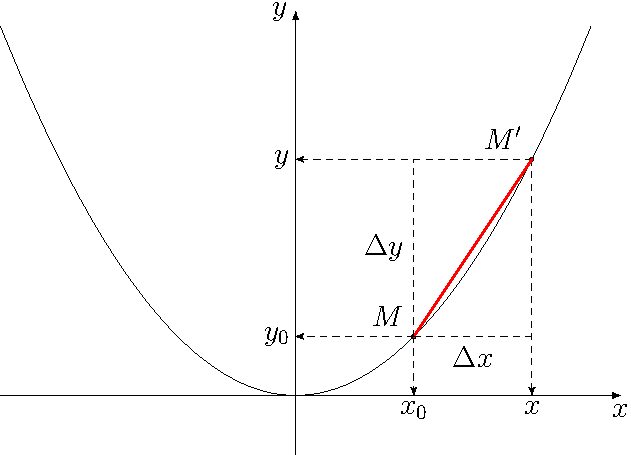
\includegraphics[page=1,scale=0.75]{analytic_geometry/int2.pdf}
	\caption{Hệ số góc (trường hợp 1)}
	\label{int2a}
\end{figure}

Tiếp theo, xét hình \ref{int2b}, ta thấy đường thẳng $MM'$ ngày càng tiến sát lại với đường cong. Như vậy, khi $\Delta x$ tiến tới 0 thì đường thẳng $MM'$ cắt đường cong tại hai điểm càng sát nhau. Đến khi hai điểm đó trùng nhau, đường thẳng $MM'$ chỉ đi qua đúng một điểm thuộc đường cong và khi đó $MM'$ trở thành tiếp tuyến của đường cong tại điểm $M = (x_0, y_0)$.

\begin{figure}[ht]
	\centering
	\includegraphics[page=2,scale=0.75]{analytic_geometry/int2.pdf}
	\caption{Hệ số góc (trường hợp 2)}
	\label{int2b}
\end{figure}

Khi đó $f'(x_0)$ là tangent của góc hợp bởi $MM'$ và trục hoành $Ox$, hay nói cách khác là \textit{hệ số góc} của đường tiếp tuyến. Thêm nữa $f'(x_0) = \dfrac{\Delta y}{\Delta x} = \dfrac{y - y_0}{x - x_0}$ nên phương trình đường tiếp tuyến đi qua $M = (x_0, y_0)$ là
\begin{equation}
	y = f'(x_0) (x - x_0) + y_0
\end{equation}

\section{Tích phân}

Tích phân là khái niệm quan trọng trong giải tích. Sau đây sẽ trình bày cách tính tích phân theo tổng Riemann.

\subsection*{Tích phân và phân chia diện tích}

Xét phương trình của một đường cong $y = f(x) > 0$ trên đoạn $[a, b]$.

Theo định nghĩa, tích phân từ $a$ tới $b$ là diện tích phần hình phẳng giới hạn bởi đường cong $y = f(x)$, trục hoành $Ox$ và hai trục đứng $x = a$, $x = b$.

Ờ hình \ref{int1}, diện tích phần tô màu xám là tích phân từ -2 tới 2 của hàm số $f(x) = -x^2 + 4$.

\begin{figure}[ht]
	\centering
	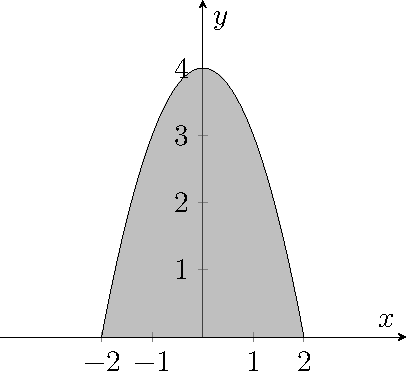
\includegraphics[page=1]{analytic_geometry/int1.pdf}
	\caption{Tích phân từ -2 tới 2 của $f(x) = -x^2 + 4$}
	\label{int1}
\end{figure}

Chúng ta có thể tính diện tích hình chữ nhật, hình thang, hình vuông. Vậy có cách nào để tính diện tích một hình giới hạn bởi các đường cong bất kì không? Có đấy. Chúng ta sẽ tính xấp xỉ bằng tổng diện tích các hình chữ nhật.

Ví dụ với hàm số $f(x) = -x^2 + 4$ ở trên, ta chia đoạn $[a, b]$ thành $n$ phần bằng nhau \[a = x_0 < x_1 < \ldots < x_{n-1} < x_n = b\]
Trong đó $x_{i+1} - x_i$ cố định và bằng $\dfrac{b-a}{n}$.

Đối với hình \ref{int2} ta xấp xỉ bằng 7 hình chữ nhật. Đối với hình \ref{int3} ta xấp xỉ bằng 15 hình chữ nhật. Đối với hình \ref{int4} ta xấp xỉ bằng 31 hình chữ nhật. 

\begin{figure}[htb]
	\centering
	\includegraphics[page=2]{analytic_geometry/int1.pdf}
	\caption{Xấp xỉ diện tích bởi 7 hình chữ nhật}
	\label{int2}
\end{figure}

\begin{figure}[htb]
	\centering
	\includegraphics[page=3]{analytic_geometry/int1.pdf}
	\caption{Xấp xỉ diện tích bởi 15 hình chữ nhật}
	\label{int3}
\end{figure}

\begin{figure}[htb]
	\centering
	\includegraphics[page=4]{analytic_geometry/int1.pdf}
	\caption{Xấp xỉ diện tích bởi 31 hình chữ nhật}
	\label{int4}
\end{figure}

Càng dùng nhiều hình chữ nhật, tổng diện tích của chúng càng gần với diện tích cần tìm, hay là tích phân cần tìm.

Ở ba hình trên, mỗi hình chữ nhật trong đó có chiều rộng bằng nhau là $\dfrac{b-a}{n}$ với $n$ là số đoạn. Chiều dài là $f(x_i)$ với $x_i = a + \dfrac{b-a}{n} i$, $i = 1, 2, \ldots, n$ (biên sau).

Cụ thể hơn, hình chữ nhật từ $x_{i-1}$ tới $x_i$ sẽ có chiều dài là $f(x_i)$ và chiều rộng là $\dfrac{b-a}{n}$. % Việc chọn chiều dài không bắt buộc phải chọn biên sau. Chúng ta hoàn toàn có thể chọn chiều dài là $f(x_{i-1})$, hoặc $\max f(x)$, $\min f(x)$ trên đoạn $[x_{i-1}, x_i]$.

Khi đó, tổng diện tích của các hình chữ nhật là
\begin{equation}
	\sum_{i=1}^n (x_{i} - x_{i-1}) f(x_i) = \sum_{i=1}^n \frac{b-a}{n} f(x_i)
\end{equation}

Khi số lượng hình chữ nhật tăng lên tới vô hạn thì tổng diện tích sẽ tiến tới diện tích chính xác của hình cần tìm, hay nói cách khác là tích phân. Do đó kết quả sẽ là
\begin{equation}
	\int\displaylimits_{a}^{b} f(x)\,dx = \lim_{n \to \infty} \sum_{i=1}^{n} \frac{b-a}{n} f(x_i), \quad x_i = a + \frac{b-a}{n} i
\end{equation}

\subsection*{Ví dụ tính tích phân qua tổng Riemann}

Ví dụ, tính tích phân từ -2 tới 2 của hàm số $f(x) = -x^2 + 4$ ở trên. Ta có $b = 2$ và $a = -2$ nên \begin{align*}
	\frac{b-a}{n} f(x_i) = & \frac{4}{n} \Bigl(-\Bigl(-2+\frac{4}{n} i\Bigr)^2 + 4\Bigr) \\ = & \frac{4}{n}\Bigl( -4 + \frac{16}{n} i - \frac{16}{n^2} i^2 + 4\Bigr) \\ = & \frac{64}{n} \Bigl( \frac{i}{n} - \frac{i^2}{n^2} \Bigr)
\end{align*}

Tính tổng $i$ từ 1 tới $n$ ta có $\displaystyle{\sum_{i=1}^{n} i = \frac{n(n+1)}{2}}$.

Tính tổng $i^2$ từ 1 tới $n$ ta có $\displaystyle{\sum_{i=1}^{n} i^2 = \frac{n(n+1)(2n+1)}{6}}$.

Suy ra
\begin{align*}
	\sum_{i=1}^n \frac{64}{n} \Bigl(\frac{i}{n} - \frac{i^2}{n^2}\Bigr) = & \frac{64}{n^2} \sum_{i=1}^n i - \frac{64}{n^3} \sum_{i=1}^{n} i^2 \\ & = -\frac{64}{n^2} \cdot \frac{n(n+1)}{2} - \frac{64}{n^3} \cdot \frac{n(n+1)(2n+1)}{6}
\end{align*}

Khi $n$ tiến tới vô cực thì biểu thức trên tiến tới $\dfrac{64}{2} - \dfrac{64 \cdot 2}{6} = \dfrac{32}{3}$. Đây chính là giá trị của tích phân $\displaystyle{\int\displaylimits_{-2}^2 (-x^2 + 4) \, dx}$.

\chapter{Hình học affine}

\section{Không gian affine}

\subsection*{Không gian affine}

\begin{definition}[Không gian affine]
	Cho $\Vv$ là một không gian vector trên trường $\FF$, và $\Aa$ là một tập khác rỗng mà các phần tử của nó gọi là \textbf{điểm}. Giả sử có ánh xạ $\varphi$
	\begin{align*}
		\varphi: \Aa \times \Aa & \to \Vv \\ (M, N) & \to \varphi(M, N)
	\end{align*} 
	thỏa mãn hai điều kiện sau
	\begin{enumerate}
		\item Với mọi điểm $M \in \Aa$ và vector $\overrightarrow{v} \in \Vv$ có duy nhất một điểm $N \in \Aa$ sao cho $\varphi(M, N) = \overrightarrow{v}$;
		\item Với ba điểm $M$, $N$, $P$ bất kì ta luôn có \[\varphi(M,N) + \varphi(N,P) = \varphi(M,P). \]
	\end{enumerate}
	
	Ta nói $\Aa$ là một \textbf{không gian affine}.
    
    Tên gọi đầy đủ: \textbf{$\Aa$ là không gian affine trên trường $\FF$ liên kết với không gian vector $\Vv$ bởi ánh xạ liên kết $\varphi$}.
\end{definition}

Khi đó, $\Vv$ được gọi là \textbf{không gian vector liên kết} với (hay \textbf{không gian nền}) của $\Aa$ và được ký hiệu là $\overrightarrow{\Aa}$.

$\varphi$ được gọi là \textbf{ánh xạ liên kết}. Ta ký hiệu $\varphi(M, N) = \overrightarrow{MN}$ từ đây về sau. Khi đó hai điều kiện trên được viết lại là

\begin{enumerate}
	\item Với mọi $M \in \Aa$, với mọi $\overrightarrow{v} \in \Vv$, tồn tại duy nhất $N \in \Aa$ sao cho $\overrightarrow{MN} = \overrightarrow{v}$
	\item Với mọi $M$, $N$, $P$ thuộc $\Aa$, $\overrightarrow{MN} + \overrightarrow{NP} = \overrightarrow{MP}$
\end{enumerate}

Biểu thức ở điều kiện 2 còn được gọi là \textbf{hệ thức Chales}.

Nếu $\FF = \RR$ thì ta gọi là không gian affine thực.

Nếu $\FF = \CC$ thì ta gọi là không gian affine phức.

Nếu muốn nhấn mạnh trường $\FF$ ta nói là $\FF$-không gian affine.

Ta ký hiệu một không gian affine là bộ $(\Aa, \overrightarrow{\Aa}, \varphi)$. Ta cũng có thể ghi tắt là $\Aa(\FF)$ hoặc chỉ là $\Aa$.

Nếu $\overrightarrow{\Aa}$ là không gian vector $n$ chiều thì ta nói $\Aa$ là không gian affine $n$ chiều và ký hiệu là $\Aa^n$. Như vậy \[\dim \Aa = \dim \overrightarrow{\Aa}\]

\begin{example}
	Xét tập hợp các điểm trong không gian $\RR^3$ học ở THTP. Khi đó $\Aa = \RR^3$ là tập hợp các điểm, $\overrightarrow{\Aa}$ là tập hợp các vector trong $\RR^3$. Một vector từ điểm $A$ tới điểm $B$ (theo nghĩa hình học) là một đoạn thẳng có hướng nối từ $A$ tới $B$.
\end{example}

\textbf{Lưu ý}. Ở THPT chúng ta học rằng tọa độ của một điểm $M$ cũng chính là tọa độ của vector $\overrightarrow{OM}$. Tuy nhiên điều đó không phải lúc nào cũng đúng. Ở các phần sau sẽ giải thích lý do tại sao.

\textbf{Tính chất của không gian affine}

Với mọi $M$, $N$, $Q$ thuộc $\Aa$ ta có

\begin{enumerate}
	\item $\overrightarrow{MN} = \overrightarrow{0}$ khi và chỉ khi $M \equiv N$
	\item $\overrightarrow{MN} = -\overrightarrow{NM}$
	\item $\overrightarrow{MN} = \overrightarrow{PQ}$ khi và chỉ khi $\overrightarrow{MP} = \overrightarrow{NQ}$
	\item $\overrightarrow{MN} = \overrightarrow{PN} - \overrightarrow{PM}$
\end{enumerate}

\begin{proof}
	Để chứng minh các tính chất trên ta sử dụng hai điều kiện trong định nghĩa không gian affine (đặc biệt là hệ thức Chales).
	
    1. Nếu $M \equiv N$ thì $\overrightarrow{MM} = \overrightarrow{MN} + \overrightarrow{NM} = \overrightarrow{MM} + \overrightarrow{MM}$. Suy ra $\overrightarrow{MM} = \overrightarrow{0}$ hay $\overrightarrow{MN} = \overrightarrow{0}$. Từ đây, nếu $\overrightarrow{MN} = \overrightarrow{0}$ thì theo điều kiện 1 trong định nghĩa, tồn tại duy nhất điểm $N$ thỏa $\overrightarrow{MN} = \overrightarrow{0}$. Điều này tương đương với $M \equiv N$.

    2. Từ hệ thức Chales ta có 
    \begin{equation*}
        \overrightarrow{0} = \overrightarrow{MM} = \overrightarrow{MN} + \overrightarrow{NM} \Leftrightarrow \overrightarrow{MN} = -\overrightarrow{NM}
    \end{equation*}
	
    3. $\overrightarrow{MN} = \overrightarrow{MP} + \overrightarrow{PN}$ và $\overrightarrow{PQ} = \overrightarrow{PN} + \overrightarrow{NQ}$ nên $\overrightarrow{MP} + \overrightarrow{PN} = \overrightarrow{PN} + \overrightarrow{NQ}$, hay $\overrightarrow{MP} = \overrightarrow{NQ}$.
	
    4. $\overrightarrow{PM} + \overrightarrow{MN} = \overrightarrow{PN}$, chuyển vế $\overrightarrow{PM}$ ta có điều phải chứng minh.
\end{proof}

\subsection*{Phẳng}

Ở THPT ta có điểm tương đương 0-phẳng, đường thẳng tương đương 1-phẳng, mặt phẳng tương đương 2-phẳng.

Trong mặt phẳng $Oxy$, một đường thẳng được xác định khi biết một điểm thuộc nó và một vector chỉ phương $\overrightarrow{v} \neq \overrightarrow{0}$. Khi đó đường thẳng đi qua $P$ nhận $\overrightarrow{v}$ làm vector chỉ phương là tập hợp các điểm $M \in \RR^2$ sao cho $\overrightarrow{PM}$ cùng phương $\overrightarrow{v}$. Nói cách khác \[d = \{ M \in \RR^2: \, \overrightarrow{PM} = a \overrightarrow{v},\, a \in \RR \}\]

Trong không gian $Oxyz$, tương tự một đường thẳng xác định khi biết một điểm thuộc nó và một vector chỉ phương $\overrightarrow{v}$ tương ứng \[d = \{ M \in \RR^3:\, \overrightarrow{PM} = a \overrightarrow{v},\, a \in \RR \}\]
Một mặt phẳng trong $\RR^3$ xác định khi biết một điểm thuộc nó và một cặp vector chỉ phương $\overrightarrow{u}$, $\overrightarrow{v}$ của nó \[\alpha = \{ M \in \RR^3:\, \overrightarrow{PM} = a \overrightarrow{u} + b \overrightarrow{v}, \, a, b \in \RR \}\]
Trong hình học affine ta mở rộng các khái niệm phẳng trên.

\begin{definition}[Phẳng]
	Cho không gian affine $(\Aa, \overrightarrow{\Aa}, \varphi)$, $P$ là một điểm thuộc $\Aa$ và $\overrightarrow{\alpha}$ là một không gian vector con của $\overrightarrow{\Aa}$. Khi đó tập hợp 
    \begin{equation*}
        \alpha = \{ M \in \Aa: \, \overrightarrow{PM} \in \alpha\}
    \end{equation*}
    được gọi là \textbf{phẳng} đi qua $P$ với (không gian chỉ) phương $\overrightarrow{\alpha}$.
\end{definition}

Nếu $\dim \overrightarrow{\alpha} = m$ thì ta nói $\alpha$ là một \textbf{phẳng $m$ chiều} hay một $m$-phẳng và viết $\dim \alpha = m$. Như vậy \[\dim \alpha = \dim \overrightarrow{\alpha}\]

Theo cách gọi thông thường, 1-phẳng là đường thẳng, 2-phẳng là mặt phẳng. \textbf{Siêu phẳng} là tên gọi của phẳng có đối chiều 1, tức là nếu số chiều của không gian là $n$ thì số chiều của siêu phẳng là $n-1$.

Chúng ta có một số nhận xét sau.

\begin{enumerate}
	\item Nếu $\alpha$ là phẳng đi qua $P$ thì $P \in \alpha$ và với mọi $M$, $N$ thuộc $\alpha$ ta có $\overrightarrow{MN} = \overrightarrow{PN} - \overrightarrow{PM}$ cũng thuộc $\alpha$;
	\item 0-phẳng là tập chỉ gồm một điểm. Do đó ta có thể xem một điểm là một 0-phẳng;
	\item Điểm $P$ trong định nghĩa không có vai trò quan trọng gì. Mọi điểm $P$ trong $\alpha$ đều có ý nghĩa như nhau;
	\item Giả sử $\alpha$ là phẳng đi qua $P$ với phương $\overrightarrow{\alpha}$, $\beta$ là phẳng đi qua $Q$ với phương $\overrightarrow{\beta}$. Khi đó $\alpha \subset \beta$ khi và chỉ khi $P \in \beta$ và $\overrightarrow{\alpha} \subset \overrightarrow{\beta}$. Suy ra $\alpha \equiv \beta$ khi $P \in \beta$ (hay $Q \in \alpha$) và $\overrightarrow{\alpha} \equiv \overrightarrow{\beta}$;
	\item Nếu $\alpha$ là phẳng với phương $\overrightarrow{\alpha}$ thì $\alpha$ được gọi là không gian affine liên kết với $\overrightarrow{\alpha}$ bởi ánh xạ liên kết
    \begin{equation*}
        \varphi_{\alpha \times \alpha}: \alpha \times \alpha \to \overrightarrow{\alpha}
    \end{equation*}
	Vì vậy ta có thể xem phẳng là không gian affine con.
\end{enumerate}

Để xác định đường thẳng ta chỉ cần biết một vector chỉ phương là đủ. Để xác định mặt phẳng ta chỉ cần biết hai vector không song song của mặt phẳng đó là đủ. Tổng quát, để xác định phương $\overrightarrow{\alpha}$ của $m$-phẳng $\alpha$ ta chỉ cần biết một cơ sở là đủ.

Từ định nghĩa của không gian vector (tập sinh) ta thấy rằng một $m$-phẳng chỉ có một không gian chỉ phương duy nhất, nhưng có thể có nhiều cơ sở khác nhau.

\subsection*{Độc lập affine và phụ thuộc affine}

\begin{definition}
	Hệ $m+1$ điểm $\{A_0, A_1, \ldots, A_m\}$ ($m \geq 1$) của không gian affine $\Aa$ được gọi là \textbf{độc lập affine} nếu hệ $m$ vector 
    \begin{equation*}
        \{\overrightarrow{A_0 A_1}, \overrightarrow{A_0 A_2}, \ldots, \overrightarrow{A_0 A_m}\}
    \end{equation*}
    của $\overrightarrow{\Aa}$ là một hệ vector độc lập tuyến tính.
	
	Hệ điểm không độc lập tuyến tính được gọi là \textbf{phụ thuộc affine}.
\end{definition}

Chúng ta có một số lưu ý từ định nghĩa.

\begin{enumerate}
	\item Tập chỉ gồm một điểm $A_0$ bất kì được quy ước là luôn độc lập;
	\item Trong định nghĩa trên điểm $A_0$ bình đẳng như các điểm khác vì nếu hệ
    \begin{equation*}
        \{\overrightarrow{A_0 A_1}, \overrightarrow{A_0 A_2}, \ldots, \overrightarrow{A_0 A_m}\}
    \end{equation*}
    độc lập affine thì hệ
    \begin{equation*}
        \{\overrightarrow{A_i A_0}, \ldots, \overrightarrow{A_i A_{i-1}}, \overrightarrow{A_i A_{i+1}}, \ldots, \overrightarrow{A_i A_m}\}
    \end{equation*}
    cũng độc lập affine;
	\item Hệ $\{A_0, \ldots, A_m\}$ phụ thuộc affine thì hệ
    \begin{equation*}
        \{\overrightarrow{A_0 A_1}, \ldots, \overrightarrow{A_0 A_m}\}
    \end{equation*}
    phụ thuộc affine;
	\item Hệ con của một hệ độc lập thì độc lập, nhưng hệ con của một hệ phụ thuộc chưa chắc phụ thuộc.
\end{enumerate}

Ta sẽ chứng minh lưu ý thứ hai.

\begin{proof}
	Ta xét tổ hợp tuyến tính \[\lambda_1 \overrightarrow{A_0 A_1} + \lambda_2 \overrightarrow{A_0 A_2} + \ldots + \lambda_m \overrightarrow{A_0 A_m}\]
	Do hệ vector độc lập tuyến tính nên $\lambda_1 = \ldots = \lambda_m = 0$. Khi đó ta khai triển vế trái
	\begin{align*}
		& \lambda_1 \overrightarrow{A_0 A_1} + \lambda_2 \overrightarrow{A_0 A_2} + \ldots + \lambda_m \overrightarrow{A_0 A_m} \\ = & \lambda_1 (\overrightarrow{A_i A_1} - \overrightarrow{A_i A_0}) + \lambda_2 (\overrightarrow{A_i A_2} - \overrightarrow{A_i A_0}) + \ldots \\ & + \lambda_{i-1} (\overrightarrow{A_i A_{i-1}} - \overrightarrow{A_i A_0}) - \lambda_i \overrightarrow{A_i A_0} + \lambda_{i+1} (\overrightarrow{A_i A_{i+1}} - \overrightarrow{A_i A_0}) \\ & + \lambda_m (\overrightarrow{A_i A_m} - \overrightarrow{A_i A_0}) \\ = & \lambda_1 \overrightarrow{A_i A_1} + \lambda_2 \overrightarrow{A_i A_2} + \ldots + \lambda_{i-1} \overrightarrow{A_i A_{i-1}} + \lambda_{i+1} \overrightarrow{A_i A_{i+1}} + \ldots \\ & + \lambda_m \overrightarrow{A_i A_m} - (\lambda_1 + \lambda_2 + \ldots + \lambda_m) \overrightarrow{A_i A_0} = \overrightarrow{0}
	\end{align*}
	
	Do $\lambda_1 = \ldots = \lambda_m = 0$ nên tổ hợp tuyến tính ứng với các vector $\overrightarrow{A_i A_j}$ ($j \neq i$) độc lập tuyến tính và ta có điều phải chứng minh.
\end{proof}

\begin{theorem}
	Trong không gian affine $n$ chiều $\Aa^n$, với $0 < m \leq n+1$, luôn tồn tại các hệ $m$ điểm độc lập. Mọi hệ gồm hơn $n+1$ điểm đều phụ thuộc.
\end{theorem}

\subsection*{Giao của các phẳng. Bao affine}

Cho $\{\alpha_i: i \in I\}$ là một họ không rỗng các phẳng trong không gian affine $\Aa$.

\begin{theorem}
	Nếu $\displaystyle{\bigcap_{i \in I} \alpha_i \neq \emptyset}$ thì $\displaystyle{\bigcap_{i \in I} \alpha_i}$ là một phẳng có phương $\displaystyle{\bigcap_{i \in I}\overrightarrow{\alpha_i}}$.
	\label{theorem2}
\end{theorem}

\begin{proof}
	Vì $\bigcap_{i \in I} \alpha_i \neq \emptyset$ nên tồn tại $P \in \bigcap_{i \in I} \alpha_i$, hay $P \in \alpha_i$ với $i \in I$.
	
	Nếu $\displaystyle{M \in \bigcap_{i \in I}}$ thì $M \in \alpha_i$ với $i \in I$. Suy ra $\overrightarrow{PM} \in \alpha_i$. Do đó 
    \begin{equation*}
        \displaystyle{\bigcap_{i \in I} \alpha_i = \{ M \in \Aa: \overrightarrow{PM} \in \bigcap_{i \in I} \overrightarrow{\alpha_i}\}}
    \end{equation*}
	
	Điều này nghĩa là $\displaystyle{\bigcap_{i \in I} \alpha_i}$ là phẳng đi qua $P$ với không gian chỉ phương là $\displaystyle{\bigcap_{i \in I} \overrightarrow{\alpha_i}}$.
\end{proof}

\begin{definition}[Phẳng giao]
	Phẳng $\displaystyle{\bigcap_{i \in I} \alpha_i}$ trong định lý trên được gọi là \textbf{phẳng giao} của các phẳng $\alpha_i$.
\end{definition}

Từ định nghĩa trên ta thấy rằng $\displaystyle{\bigcap_{i \in I} \alpha_i}$ là phẳng lớn nhất (theo quan hệ bao hàm) chứa trong tất cả các phẳng $\alpha_i$, $i \in I$.

\begin{definition}[Bao affine]
	Cho $X$ là một tập con khác rỗng của không gian affine $\Aa$. Khi đó giao của mọi phẳng chứa $X$ trong $\Aa$ sẽ là một phẳng, gọi là \textbf{bao affine} của $X$, ký hiệu là $\langle X \rangle$.
\end{definition}

Như vậy, bao affine $\langle X \rangle$, theo quan hệ bao hàm, của tập $X$ là phẳng bé nhất chứa $X$.

Tương tự phép giao và hợp của hai tập hợp, chúng ta có phép giao các phẳng ở trên và phép tổng của các phẳng sẽ đề cập sau đây.

\begin{definition}[Phẳng tổng]
	Cho $\{ \alpha_i: i \in I \}$ là một họ không rỗng các phẳng. Bao affine của tập hợp $\displaystyle{\bigcup_{i \in I} \alpha_i}$ được gọi là \textbf{phẳng tổng} (hay \textbf{tổng}) của các phẳng $\alpha_i$, ký hiệu là $\displaystyle{\sum_{i \in I} \alpha_i}$.
\end{definition}

Như vậy, phẳng tổng là phẳng bé nhất chứa tất cả các phẳng $\alpha_i$, $i \in I$. 

Ta có nhận xét sau. Nếu $X$ là một hệ hữu hạn điểm $X = \{P_0, P_1, \ldots, P_m \}$ thì tổng $P_0 + P_1 + \ldots + P_m$ (ta xem các $P_i$ là các 0-phẳng) là phẳng có số chiều bé nhất đi qua các điểm này. Hơn nữa \[\dim (P_0 + P_1 + \ldots + P_m) = \text{rank} \{ \overrightarrow{P_0 P_1}, \overrightarrow{P_0 P_2}, \ldots, \overrightarrow{P_0 P_m} \}\]

Do đó hệ điểm $\{ P_0, P_1, \ldots, P_m \}$ độc lập thì $\dim (P_0 + P_1 + \ldots + P_m) = m$.

\begin{proof}
	Đặt $I = P_0 + P_1 + \ldots + P_m$ là phẳng tổng của hệ điểm \[ \{P_0, P_1, \ldots, P_m\} \]
    
    Khi đó $I$ đi qua các điểm $P_0$, $P_1$, ..., $P_m$.
	
	Đặt $\alpha_i$ là phẳng đi qua $P_0$ và $P_i$, $i = 1, 2, \ldots, m$. Khi đó $\alpha_i$ có phương là $\overrightarrow{P_0 P_i}$. Tổng $I$ chính là tổng các phẳng $\alpha_1 + \alpha_2 + \ldots + \alpha_m$, và $\overrightarrow{P_0 P_1}$, $\overrightarrow{P_0 P_2}$, ..., $\overrightarrow{P_0 P_m}$ là các vector chỉ phương của nó. Như vậy nếu $\overrightarrow{I}$ là không gian chỉ phương của $I$ thì nó gồm các vector độc lập tuyến tính $\overrightarrow{P_0 P_{i_1}}$, $\overrightarrow{P_0 P_{i_2}}$, ..., $\overrightarrow{P_0 P_{i_k}}$. Khi đó $\dim I = \dim \overrightarrow{I} = k = \text{rank} \{ \overrightarrow{P_0 P_1}, \overrightarrow{P_0 P_2}, \ldots, \overrightarrow{P_0 P_m}\}$. Từ đây ta có điều phải chứng minh.
\end{proof}

\begin{theorem}
	Cho $\alpha$ và $\beta$ là hai phẳng. Nếu $\alpha \cap \beta \neq \emptyset$ thì với mọi $P \in \alpha$ và với mọi $Q \in \beta$ ta có $\overrightarrow{PQ} = \overrightarrow{\alpha} + \overrightarrow{\beta}$.
    
    Ngược lại nếu có điểm $P \in \alpha$ và $Q \in \beta$ sao cho $\overrightarrow{PQ} = \overrightarrow{\alpha} + \overrightarrow{\beta}$ thì $\alpha \cap \beta \neq \emptyset$.
	\label{theorem3}
\end{theorem}

\begin{proof}
	Giả sử $\alpha \cap \beta \neq \emptyset$. Khi đó tồn tại điểm $M \in \alpha \cap \beta$, suy ra $M \in \alpha$ và $M \in \beta$. Với mọi $P \in \alpha$ và với mọi $Q \in \beta$ thì $\overrightarrow{PM} \in \overrightarrow{\alpha}$ và $\overrightarrow{MQ} \in \overrightarrow{\beta}$. Từ đó $\overrightarrow{PQ} = \overrightarrow{PM} + \overrightarrow{MQ} = \overrightarrow{\alpha} + \overrightarrow{\beta}$.
	
	Đảo lại, giả sử ta có điểm $P \in \alpha$ và điểm $Q \in \beta$ sao cho $\overrightarrow{PQ} = \overrightarrow{\alpha} + \overrightarrow{\beta}$. Khi đó tồn tại hai vector $\overrightarrow{u}$ và $\overrightarrow{v}$ sao cho $\overrightarrow{PQ} = \overrightarrow{u} + \overrightarrow{v}$ với $\overrightarrow{u} \in \overrightarrow{\alpha}$ và $\overrightarrow{v} \in \overrightarrow{\beta}$. Theo định nghĩa của không gian affine thì với điểm $P \in \alpha$, tồn tại duy nhất điểm $M \in \alpha$ sao cho $\overrightarrow{PM} = \overrightarrow{u}$. Tương tự với điểm $Q \in \beta$ tồn tại duy nhất điểm $N \in \beta$ sao cho $\overrightarrow{QN} = \overrightarrow{v}$. Suy ra $\overrightarrow{PQ} = \overrightarrow{u} + \overrightarrow{v} = \overrightarrow{PM} - \overrightarrow{QN}$. Chuyển vế $\overrightarrow{QN}$ ta có $\overrightarrow{PM} = \overrightarrow{u} = \overrightarrow{PQ} + \overrightarrow{QN} = \overrightarrow{PN}$. Điều này chỉ xảy ra khi $M \equiv N$, hay nói cách khác $M$ và $N$ thuộc $\alpha \cap \beta$. Như vậy $\alpha \cap \beta \neq \emptyset$.
\end{proof}

\begin{theorem}
	Giả sử $\alpha$ và $\beta$ là hai phẳng với phương lần lượt là $\overrightarrow{\alpha}$ và $\overrightarrow{\beta}$. Khi đó
	
	\begin{enumerate}[nosep,leftmargin=*]
		\item Nếu $\alpha \cap \beta \neq \emptyset$ thì
        \begin{equation*}
            \dim(\alpha + \beta) = \dim(\alpha) + \dim(\beta) - \dim(\alpha \cap \beta)
        \end{equation*}
		\item Nếu $\alpha \cap \beta = \emptyset$ thì
        \begin{equation*}
            \dim(\alpha + \beta) = \dim(\alpha) + \dim(\beta) - \dim(\overrightarrow{\alpha} \cap \overrightarrow{\beta}) + 1
        \end{equation*}
	\end{enumerate}
\end{theorem}

\begin{proof}
	1. Nếu $\alpha \cap \beta \neq \emptyset$ thì theo định lý \ref{theorem2} ta có $\alpha \cap \beta$ là một phẳng có phương $\overrightarrow{\alpha} \cap \overrightarrow{\beta}$. Lấy $P \in \alpha \cap \beta$ và gọi $\gamma$ là phẳng đi qua $P$ với phương $\overrightarrow{\gamma} = \overrightarrow{\alpha} + \overrightarrow{\beta}$. Ta có $\alpha \subset \gamma$ và $\beta \subset \gamma$. Ngoài ra nếu có phẳng $\gamma'$ chứa $\alpha$ và $\beta$ thì $P \in \gamma'$ và phương của $\gamma'$ phải chứa $\overrightarrow{\alpha}$ và $\overrightarrow{\beta}$. Nói cách khác $\gamma \subset \gamma'$. Vậy $\gamma$ là phẳng bé nhất chứa $\alpha$ và $\beta$, tức là $\gamma = \alpha + \beta$. Do đó 
    \begin{align*}
        \dim(\alpha + \beta) = & \dim\gamma = \dim\overrightarrow{\gamma} = \dim(\alpha + \beta) \\ 
        = & \dim\overrightarrow{\alpha} + \dim\overrightarrow{\beta} - \dim(\overrightarrow{\alpha} \cap \overrightarrow{\beta}) \\ 
        = & \dim\alpha + \dim\beta - \dim(\overrightarrow{\alpha} \cap \overrightarrow{\beta})
    \end{align*}
	
    2. Nếu $\alpha \cap \beta = \emptyset$ thì theo định lý \ref{theorem3}, nếu ta lấy $P \in \alpha$ và $Q \in \beta$ thì $\overrightarrow{PQ} \not\in \overrightarrow{\alpha} + \overrightarrow{\beta}$. Gọi $\overrightarrow{\gamma}$ là không gian con một chiều sinh bởi $\overrightarrow{PQ}$, ta có $(\overrightarrow{\alpha} + \overrightarrow{\beta}) \cap \overrightarrow{\gamma} = \{ \overrightarrow{0} \}$ (các không gian vector không có vector nào chung ngoài $\overrightarrow{0}$). Gọi $\eta$ là phẳng đi qua $P$ có không gian chỉ phương là $\overrightarrow{\alpha} + \overrightarrow{\beta} + \overrightarrow{\gamma}$ thì ta có $\alpha \subset \eta$ và $\beta \subset \eta$. Suy ra $\alpha + \beta \subset \eta$.
		
	3. $\eta'$ là một phẳng chứa $\alpha$ và $\beta$ thì $P \in \eta'$ và phương $\overrightarrow{\eta'}$ của $\eta'$ phải chứa $\overrightarrow{\alpha}$, $\overrightarrow{\beta}$ và $\overrightarrow{\gamma}$. Từ đó $\eta \subset \eta'$. Suy ra $\eta$ là phẳng bé nhất chứa $\alpha$ và $\beta$, hay $\eta = \alpha + \beta$. Do $\dim((\overrightarrow{\alpha} + \overrightarrow{\beta}) \cap \overrightarrow{\gamma}) = 0$ nên
    \begin{align*}
        \dim(\alpha + \beta) = & \dim\eta = \dim(\overrightarrow{\alpha} + \overrightarrow{\beta} + \overrightarrow{\gamma}) \\ 
        = & \dim\overrightarrow{\alpha} + \dim\overrightarrow{\beta} + \dim\overrightarrow{\gamma} - \dim(\overrightarrow{\alpha} \cap \overrightarrow{\beta}) \\ 
        = & \dim\alpha + \dim\beta + 1 - \dim(\overrightarrow{\alpha} \cap \overrightarrow{\beta})
    \end{align*}

    Như vậy ta có công thức tính số chiều của phẳng giao.
\end{proof}

\subsection*{Vị trí tương đối}

\begin{definition}[Cắt nhau, chéo nhau, song song]
    Hai phẳng $\alpha$ và $\beta$ được gọi là \textbf{cắt nhau cấp $r$} nếu $\alpha \cap \beta$ là một $r$-phẳng. 
    
    Chúng được gọi là \textbf{chéo nhau cấp $r$} nếu $\alpha \cap \beta = \emptyset$ và $\dim(\overrightarrow{\alpha} \cap \overrightarrow{\beta}) = r$. 
    
    Chúng được gọi là \textbf{song song} (với nhau) nếu $\overrightarrow{\alpha} \subset \overrightarrow{\beta}$ hoặc $\overrightarrow{\beta} \subset \overrightarrow{\alpha}$. 
\end{definition}

Theo định lý về dim bên trên, trong $\RR^3$ không tồn tại hai mặt phẳng chéo nhau cấp 0 hoặc 1.

\begin{theorem}
    \label{theorem5}
    Cho hai phẳng  song song $\alpha$ và $\beta$. Nếu $\alpha \cap \beta \neq \emptyset$ thì $\alpha \subset \beta$ hoặc $\beta \subset \alpha$.
\end{theorem}

\begin{proof}
	Do $\alpha$ và $\beta$ có điểm chung nên $\alpha \cap \beta$ là một phẳng có phương $\overrightarrow{\alpha} \cap \overrightarrow{\beta}$. Theo định nghĩa về sự song song, $\alpha$ song song $\beta$ dẫn tới $\overrightarrow{\alpha} \subset \overrightarrow{\beta}$ hoặc $\overrightarrow{\beta} \subset \overrightarrow{\alpha}$. Nếu $\overrightarrow{\alpha} \subset \overrightarrow{\beta}$ thì $\overrightarrow{\alpha} \cap \overrightarrow{\beta} = \overrightarrow{\alpha}$. Suy ra $\alpha \cap \beta = \alpha$ hay $\alpha \subset \beta$. Trường hợp $\overrightarrow{\beta} \subset \overrightarrow{\alpha}$ tương tự.
\end{proof}

\begin{theorem}
    Qua một điểm $A$ có một và chỉ một $m$-phẳng song song với $m$-phẳng $\alpha$ đã cho.
\end{theorem}

\begin{proof}
	Gọi $\beta$ là $m$-phẳng đi qua $A$ với phương là $\overrightarrow{\alpha}$. Khi đó $\beta$ là phẳng $m$ chiều song song với $\alpha$. Nếu $\beta'$ cũng là $m$-phẳng đi qua $A$ và song song với $\alpha$ thì $\overrightarrow{\beta'} = \overrightarrow{\beta} = \overrightarrow{\alpha}$. Do $\beta$ và $\beta'$ có điểm chung nên theo định lý \ref{theorem5} ta có $\beta \equiv \beta'$
\end{proof}

\begin{theorem}
    Trong không gian affine $n$ chiều $\Aa^n$ cho một siêu phẳng $\alpha$ và một $m$-phẳng $\beta$ ($1 \leq m \leq n-1$). Khi đó $\alpha$ và $\beta$ hoặc song song hoặc cắt nhau theo một $(m-1)$-phẳng.
\end{theorem}

\subsection*{Mục tiêu và tọa độ affine}

\begin{definition}[Mục tiêu affine]
    Cho $\Aa^n$ là một không gian affine $n$ chiều. Hệ $\{O, \overrightarrow{e_1}, \overrightarrow{e_2}, \ldots, \overrightarrow{e_n}\}$ gồm một điểm $O \in \Aa^n$ và một cơ sở $\{\overrightarrow{e_1}, \overrightarrow{e_2}, \ldots, \overrightarrow{e_n}\}$ của $\overrightarrow{\Aa^n}$ được gọi là \textbf{mục tiêu affine} (hay \textbf{mục tiêu}) của $\Aa^n$.
    
    Điểm $O$ được gọi là \textbf{gốc}, vector $\overrightarrow{e_i}$ được gọi là \textbf{vector cơ sở thứ $i$}, $i = 1, 2, \ldots, n$. 
\end{definition}

Giả sử $\{O, \overrightarrow{e_i}\}$ là một mục tiêu của không gian affine $\Aa^n$. Khi đó với mọi $M \in \Aa^n$, vector $\overrightarrow{OM} \in \overrightarrow{\Aa^n}$ nên ta có biểu diễn tuyến tính của $\overrightarrow{OM}$ qua các cơ sở $\{\overrightarrow{e_i}\}$ \[\overrightarrow{OM} = \sum_{i=1}^n x_i \overrightarrow{e_i}\]

Nhắc lại đại số tuyến tính, lúc này vector $\overrightarrow{OM}$ có tọa độ $(x_1, x_2, \ldots, x_n)$ đối với cơ sở $\{\overrightarrow{e_i}\}$, $x_i \in \FF$, $i = 1, 2, \ldots, n$.

Khi đó bộ $(x_1, x_2, \ldots, x_n)$ được gọi là \textit{tọa độ} của $M$ trong mục tiêu $\{O, \overrightarrow{e_i}\}$ và $x_i$ được gọi là tọa độ thứ $i$. Ta ký hiệu tọa độ của $M$ là $M(x_i)$ hoặc $(x_i)$.

Giả sử $M$ có tọa độ $(x_i)$ và $N$ có tọa độ $(y_i)$ đối với mục tiêu $\{\overrightarrow{e_i}\}$. Ta có $\overrightarrow{MN} = \overrightarrow{ON} - \overrightarrow{OM} = (y_i - x_i)$. Như vậy $(y_i - x_i)$ là tọa độ của vector $\overrightarrow{MN}$ trong mục tiêu $\{O, \overrightarrow{e_i}\}$.

Ta có một số nhận xét về mục tiêu affine.

\begin{enumerate}
    \item Giả sử trên $\Aa^n$ đã chọn được mục tiêu cố định $\{O, \overrightarrow{e_i}\}$. Xét ánh xạ 
    \begin{align*}
        \varphi: \, & \Aa \to \FF^n \\ & M \to (x_i)
    \end{align*}
    với $(x_i)$ là tọa độ của $M$. Khi đó $\varphi$ là song ánh và mỗi điểm được đồng nhất với một phần tử của $\FF^n$. Nói cách khác đối tượng hình học được đồng nhất với đối tượng đại số.
    \item Xét mục tiêu affine $\{O, \overrightarrow{e_i}\}$ của $\Aa^n$ và gọi $E_i \in \Aa$ là các điểm sao cho $\overrightarrow{OE_i} = \overrightarrow{e_i}$. Khi đó hệ điểm $\{O, E_1, E_2, \ldots, E_n\}$ độc lập affine. Ngược lại, một hệ gồm $n+1$ điểm $\{O, E_1, E_2, \ldots, E_n\}$ độc lập affine xác định một mục tiêu affine $\{O, \overrightarrow{e_i}\}$ với $\overrightarrow{e_i} = \overrightarrow{OE_i}$. Nếu ta chọn $O = (0, \ldots, 0)$ và $E_i = (0, \ldots, 0, 1, 0, \ldots, 0)$ với số 1 ở vị trí $i$ thì đây được gọi là cơ sở chính tắc.
    \item Siêu phẳng đi qua $n$ điểm độc lập $O$, $E_1$, $E_2$, ..., $E_{i-1}$, $E_{i+1}$, ..., $E_n$ được gọi là \textbf{siêu phẳng tọa độ thứ $i$}. Dễ thấy $M$ thuộc siêu phẳng tọa độ thứ $i$ khi và chỉ khi $x_i = 0$ với $x_i$ là tọa độ thứ $i$ của $M$.
\end{enumerate}

\chapter{Machine Learning}

\section{Các thuật toán cơ sở}

\subsection*{Linear Regression}

Giả sử ta có $N$ điểm dữ liệu đầu vào $\bm{x}_1, \bm{x}_2, \ldots, \bm{x}_N$ với $\bm{x}_i \in \RR^d$. Ứng với từng điểm dữ liệu đầu vào $\bm{x}_i$ ta có một đầu ra $y_i$. Nghĩa là ta có $N$ cặp dữ liệu $(\bm{x}_i, y_i)$.

Mục tiêu là xây dựng hàm số $\hat{y} = f(x_1, x_2, \ldots, x_d)$ sao cho tổng sai số của $y_i$ và $\hat{y}_i$ là nhỏ nhất, tức là \[ \sum_{i=1}^N \lVert y_i - \hat{y}_i \rVert^2 \to \min \]

Để hàm số đạt giá trị nhỏ nhất (hoặc lớn nhất) ta tìm cực trị của hàm số và khảo sát. Tuy nhiên không phải hàm số nào cũng đạo hàm được. Một cách tiếp cận đơn giản là sử dụng hàm tuyến tính, dễ xây dựng và luôn khả vi. Ta đặt \[ \hat{y} = f(x_1, x_2, \ldots, x_d) = w_0 + w_1 x_1 + w_2 x_2 + \ldots + w_d x_d \]

Lúc này, hàm mất mát ở trên có dạng \[ \mathcal{L} = \sum_{i=1}^N \lVert y_i - (w_0 + w_1 x_{i1} + w_2 x_{i2} + \ldots + w_d x_{id} \rVert^2 \]

Bình phương chuẩn Euclid chính là bình phương của vector. Do đó dưới dấu tổng là các hàm số bình phương. Khi đạo hàm riêng theo $w_j$ ta có \[ \dfrac{\partial \mathcal{L}}{\partial w_j} = \sum_{i=1}^N 2 x_{ij} (y_i - (w_0 + w_1 x_{i1} + w_2 x_{i2} + \ldots + w_d x_{id})) \] với $1 \leq j \leq d$. Với $j = 0$ có chút khác biệt, $\dfrac{\partial \mathcal{L}}{\partial w_0} = \sum_{i=1}^N 2 (y_i - (w_0 + w_1 x_{i1} + \ldots + w_d x_{id}))$.

Ta cho các đạo hàm riêng $\dfrac{\partial \mathcal{L}}{\partial w_j}$ bằng 0 thì được
\begin{align*}
    \sum_{i=1}^N x_{ij} (w_0 + w_1 x_{i1} + w_2 x_{i2} + \ldots + w_d x_{id}) & = \sum_{i=1}^N x_{ij} y_i \\ \Leftrightarrow w_0 \sum_{i=1}^N x_{ij} + w_1 \sum_{i=1}^N x_{ij} x_{i1} + w_2 \sum_{i=1}^N x_{ij} x_{i2} \\ + \cdots + w_d \sum_{i=1}^N x_{ij} x_{id} & = \sum_{i=1}^N x_{ij} y_i
\end{align*}

Bây giờ chúng ta cần biểu diễn các dấu tổng lại thành dạng đại số (ma trận, vector) vì chúng sẽ được sử dụng để nhân với vector $\bm{w} = (w_0, w_1, \ldots, w_d)$.

Ta có $\sum_{i=1}^N x_{ij} = \begin{pmatrix}
    1 & 1 & \cdots & 1
\end{pmatrix} \cdot \begin{pmatrix}
    x_{1j} \\ x_{2j} \\ \vdots \\ x_{Nj}
\end{pmatrix}$.

Ta cũng có $\sum_{i=1}^N x_{ij} x_{i1} = \begin{pmatrix}
    x_{11} & x_{21} & \cdots & x_{N1}
\end{pmatrix} \cdot \begin{pmatrix}
    x_{1j} \\ x_{2j} \\ \vdots \\ x_{Nj}
\end{pmatrix}$.

Cứ tương tự như vậy, ta xếp các dấu sigma thành dạng cột thì tương đương với \[\begin{pmatrix}
    * & \sum_{i=1}^N x_{ij} & * \\ * & \sum_{i=1}^N x_{ij} x_{i1} & * \\ \vdots & \vdots & \vdots \\ * & \sum_{i=1}^N x_{ij} x_{id} & *
\end{pmatrix} = \begin{pmatrix}
    1 & 1 & \cdots & 1 \\ x_{11} & x_{21} & \cdots & x_{N1} \\ \cdots & \cdots & \ddots & \cdots \\ x_{1d} & x_{2d} & \cdots & x_{Nd} 
\end{pmatrix} \cdot \begin{pmatrix}
    * & x_{1j} & * \\ * & x_{2j} & * \\ \vdots & \vdots & \vdots \\ * & x_{Nj} & *
\end{pmatrix}\]

Ghép các cột theo thứ tự $j$ từ 0 tới $d$ ta có
\begin{align*}
    \begin{pmatrix}
        w_0 & w_1 & \cdots & w_d
    \end{pmatrix} & \cdot \begin{pmatrix}
        1 & 1 & \cdots & 1 \\ x_{11} & x_{21} & \cdots & x_{N1} \\ \cdots & \cdots & \ddots & \cdots \\ x_{1d} & x_{2d} & \cdots & x_{Nd}
    \end{pmatrix} \\ & \times \begin{pmatrix}
        1 & x_{11} & \cdots & x_{1d} \\ 1 & x_{21} & \cdots & x_{2d} \\ \cdots & \cdots & \ddots & \cdots \\ 1 & x_{N1} & \cdots & x_{Nd}
    \end{pmatrix} \\ = \begin{pmatrix}
        y_1 & y_2 & \cdots & y_N
    \end{pmatrix} & \cdot \begin{pmatrix}
        1 & x_{11} & \cdots & x_{1d} \\ 1 & x_{21} & \cdots & x_{2d} \\ \cdots & \cdots & \ddots & \cdots \\ 1 & x_{N1} & \cdots & x_{Nd}
    \end{pmatrix}
\end{align*}

Hay nói cách khác, nếu ta đặt $\bm{w} = (w_0, w_1, \ldots, w_d)$ là ma trận hàng, $\bm{X}$ là ma trận có các hàng là các input, thì phương trình trên được viết lại là $\bm{w} \bm{X}^T \bm{X} = \bm{y} \bm{X}$.

Nếu đặt $\bm{A} = \bm{X}^T \bm{X}$ và $\bm{b} = \bm{y} \bm{X}$ thì đây là hệ phương trình theo các ẩn $w_0, w_1, \ldots, w_d$. Tuy nhiên không phải lúc nào $\bm{A}$ cũng khả nghịch nên chúng ta sẽ sử dụng một khái niệm gọi là \textit{giả nghịch đảo} để tìm nghiệm cho hệ phương trình.

Ký hiệu $\bm{A}^\dag$ là giả nghịch đảo của ma trận $\bm{A}$. Khi đó nghiệm của hệ phương trình là $\bm{w} = \bm{b} \bm{A}^\dag$.

\subsection*{K-Means clustering}

Một công việc thường được quan tâm là phân loại một nhóm các đối tượng thành những nhóm nhỏ hơn theo những tiêu chí nhất định.

Tương tự như phần trước, chúng ta có $N$ điểm dữ liệu $\bm{x}_i$ thuộc $\RR^d$. Ta muốn phân cụm các vector này vào những cluster (cụm) sao cho chúng gần nhau nhất (về mặt khoảng cách Euclid).

Giả sử ta muốn phân $N$ điểm dữ liệu trên vào $K < N$ cluster. Ta cần tìm các điểm $\bm{m}_1, \bm{m}_2, \ldots, \bm{m}_K$ là tâm của các cụm, sao cho tổng khoảng cách từ các điểm $\bm{x}_i$ tới tâm cluster mà nó được phân vào là nhỏ nhất. Nghĩa là ứng với center $\bm{m}_1$ ta cần tìm các điểm $\bm{x}_{i_1}, \bm{x}_{i_2}, \ldots, \bm{x}_{i_t}$ sao cho $\sum_{j=1}^t \lVert \bm{x}_{i_j} - \bm{m}_1 \rVert^2$ nhỏ nhất. Tương tự cho các tâm khác.

Nhưng câu chuyện phức tạp ở đây là, tâm nằm ở đâu để có thể bao quát các điểm? Tâm được chọn phải có tính tổng quát, và việc phân các điểm vào cluster tương ứng với tâm thực hiện như thế nào?

Một kỹ thuật thường được sử dụng là \textit{one-hot}. Với mỗi điểm dữ liệu $\bm{x}_i$ ta thêm một label $\bm{y}_i = (y_{i1}, \cdots y_{iK})$. Điểm $\bm{x}_i$ sẽ thuộc cluster $j$ khi $y_{ij} = 1$, không thuộc thì bằng 0. Như vậy chỉ có đúng một phần tử của $\bm{y}_i$ bằng 1, còn lại bằng 0. Như vậy ràng buộc của $\bm{y}_i = (y_{i1}, y_{i2}, \ldots, y_{iK})$ là $y_{ij} \in \{ 0, 1 \}$ và $\sum_{j=1}^K y_{ij} = 1$.

Khi đó, ta mong muốn phân các điểm $\bm{x}_i$ vào cluster $\bm{m}_k$ để khoảng cách tới tâm $\bm{m}_k$ là ngắn nhất, hay $\lVert \bm{x}_i - \bm{m}_k \rVert^2 \to \min$. Thêm nữa, với cách ký hiệu $y_{ij}$ như trên, biểu thức tương đương với \[ \lVert \bm{x}_i - \bm{m}_k \rVert^2 = y_{ik} \lVert \bm{x}_i - \bm{m}_k \rVert^2 = \sum_{j=1}^K y_{ij} \lVert \bm{x}_i - \bm{m}_j \rVert^2 \] vì điểm $\bm{x}_i$ sẽ thuộc cluster $\bm{m}_k$ nào đó với $1 \leq k \leq K$.

Sai số cho toàn bộ dữ liệu lúc này sẽ là \[ \mathcal{L} (\bm{Y}, \bm{M}) = \sum_{i=1}^N \sum_{j=1}^K y_{ij} \lVert \bm{x}_i - \bm{m}_j \rVert^2 \]

Ta cần tối ưu $\bm{Y}$ và $\bm{M}$. Việc tối ưu hai ma trận cùng lúc là rất khó thậm chí bất khả thi. Do đó chúng ta có một cách tiếp cận khác là luân phiên cố định một bên và tối ưu bên còn lại. Từ đó công việc được chia làm hai bước.

\underline{Bước 1. Cố định $\bm{M}$, tìm $\bm{Y}$.}

Giả sử ta đã biết các center $\bm{m}_1, \bm{m}_2, \ldots, \bm{m}_K$. Lúc này ta cần phân các điểm $\bm{x}_i$ vào cluster gần nó nhất. Dễ thấy rằng center gần nó nhất sẽ có khoảng cách Euclid ngắn nhất. Do đó ta tìm $j$ sao cho $\lVert \bm{x}_i - \bm{m}_j \rVert^2$ đạt nhỏ nhất. Không cần thiết phải tính căn bậc hai để giảm độ phức tạp.

\underline{Bước 2. Cố định $\bm{Y}$, tìm $\bm{M}$.}

Khi đã biết $\bm{Y}$ tức là ta đã biết điểm nào được phân vào cluster nào. Khi đó ta cần tìm tâm cho từng cluster. Gọi $l (\bm{m}_j)$ là hàm tổng bình phương khoảng cách các điểm trong cluster tới tâm $\bm{m}_j$. Nghĩa là \[ l (\bm{m}_j) = \sum_{i=1}^N y_{ij} \lVert \bm{x}_i - \bm{m}_j \rVert^2 \]

Mục tiêu của chúng ta là tối ưu tâm $\bm{m}_j$. Do đó ta đạo hàm theo vector $\bm{m}_j$ thu được $\dfrac{\partial l(\bm{m}_j}{\partial \bm{m}_j} = \sum_{i=1}^N 2 y_{ij} (\bm{x}_i - \bm{m}_j)$. Cho đạo hàm bằng 0 và biến đổi ta có \begin{align*}
    & 2 \sum_{i=1}^N y_{ij} (\bm{x}_i - \bm{m}_j) = 0 \\ \Leftrightarrow \, & \bm{m}_j \sum_{i=1}^N y_{ij} = \sum_{i=1}^N y_{ij} \bm{x}_i \\ \Leftrightarrow \, & \bm{m}_j = \dfrac{\sum_{i=1}^N y_{ij} \bm{x}_i}{\sum_{i=1}^N y_{ij}}
\end{align*}

Để ý rằng, $\sum_{i=1}^N y_{ij}$ là số lượng điểm trong cluster, và $\sum_{i=1}^N y_{ij} \bm{x}_i$ là tổng các điểm trong cluster. Như vậy $\bm{m}_j$ là trung bình cộng các điểm trong cluster $j$.

\begin{algorithm}
    \caption{Thuật toán K-Means clustering}
    \begin{algorithmic}
        \Require Dữ liệu $\bm{X}$ (có $N$ điểm dữ liệu) và số cluster $K$
        \Ensure Các center $\bm{M}$ và label $\bm{y}$ cho mỗi điểm dữ liệu
        \State 1. Chọn $K$ điểm bất kì làm các cluster ban đầu.
        \State 2. Phân mỗi điểm dữ liệu vào cluster gần nó nhất (cố định $M$, tìm $Y$).
        \State 3. Nếu việc phân dữ liệu vào các cluster ở bước 2 không thay đổi so với trước đó thì dừng thuật toán.
        \State 4. Cập nhật center mới cho mỗi cluster bằng cách lấy trung bình cộng các điểm trong cluster (cố định $Y$, tìm $M$).
        \State 5. Quay lại bước 2.
    \end{algorithmic}
\end{algorithm}

\subsection*{Gradient Descent}

Trong nhiều trường hợp chúng ta thường không thể tìm nghiệm của phương trình đạo hàm để từ đó tìm các cực trị địa phương. Một phương pháp hiệu quả là gradient descent.

\subsubsection*{Hàm một biến}

Giả sử $x^*$ là local extremum (cực trị địa phương) của hàm số $f(x)$. Khi đó chúng ta xây dựng dãy số $\{ x_n \}$ hội tụ về $x^*$. Ý tưởng thực hiện là dựa trên nhận xét, nếu $x_n$ nằm bên phải $x^*$ thì $x_{n+1}$ nằm giữa $x^*$ và $x_n$. Ta đã biết nếu $x^*$ là một điểm cực trị thì $f'(x) > 0$ với $x > x^*$ mà $x_n$ đi từ bên phải sang bên trái (ngược chiều $Ox$ nên mang dấu âm). Từ đó chúng ta có công thức chung sau \[x_{n+1} = x_n - \eta f'(x_n)\]

Trong đó $\eta$ là một số dương nhỏ, gọi là \textit{learning rate} (tốc độ học).

Ta chọn $x_0$ là một điểm bất kì. Tuy nhiên việc chọn $x_0$ cũng có thể ảnh hưởng đến tốc độ hội tụ.

Ví dụ với hàm số $f(x) = x^2 + 5 \sin x$. Ta có đạo hàm là $f'(x) = 2x + 5 \cos x$. Việc giải phương trình đạo hàm bằng 0 là điều không dễ dàng. Do đó gradient descent tỏ ra hiệu quả trong trường hợp này.

Chọn $\eta = 0.1$ và $x_0 = 5$. Sau đó chọn $\eta = 0.1$ và $x_0 = -5$. Ta thấy trường hợp sau tốn ít vòng lặp hơn do $x_0 = -5$ gần điểm cực trị hơn ($\approx -1.11$).

\subsubsection*{Hàm nhiều biến}

Lúc này đầu vào của hàm số là một vector $\bm{x}$. Đặt $\nabla f(\bm{x})$ là đạo hàm của hàm $f$ theo vector $\bm{x}$. Tương tự, ta xây dựng dãy vector $\{ \bm{x}_n \}$ hội tụ về cực trị $\bm{x}^*$. Công thức lúc này là \[\bm{x}_{n+1} = \bm{x}_n - \eta \cdot \nabla f(\bm{x}_n)\]

Ta đã biết đạo hàm của hàm số theo vector cũng là vector cùng cỡ. Do đó giả sử $f(\bm{x}) = f(x_1, x_2, \ldots, x_n)$ thì đạo hàm của nó là \[\nabla f(\bm{x}) = \Bigl( \dfrac{\partial f}{\partial x_1}, \dfrac{\partial f}{\partial x_2}, \ldots, \dfrac{\partial f}{\partial x_n}\Bigr)\]

Với ví dụ là bài toán Linear Regression, lúc này hàm mất mát là \[\mathcal{L} = \dfrac{1}{2N} \sum_{i=1}^N \lVert y_i - \bm{x}_i \bm{w}^T \rVert^2 = \dfrac{1}{2N} \lVert \bm{y} - \bm{X} \bm{w}^T \rVert^2\]

Đạo hàm của hàm mất mát là \[\nabla \mathcal{L} = \dfrac{1}{N} (\bm{w} \bm{X}^T - \bm{y}) \bm{X}\]

Lúc này, với vector khởi đầu $\bm{w}_0$ chúng ta xây dựng dãy $\{ \bm{w}_n \}$ tới khi nhận được $\bm{w}_n / d < \varepsilon$, với $d$ là độ dài vector $\bm{w}$.

\subsection*{Perception Learning Algorithm}

Một trong những nhiệm vụ quan trọng nhất của ML là phân loại (tiếng Anh - classification).

Perception là thuật toán phân loại cho trường hợp đơn giản nhất khi có hai lớp. Nếu ta có các điểm dữ liệu cho trước trong không gian $d$ chiều, ta muốn tìm một siêu phẳng ($(d-1)$-phẳng) chia các điểm dữ liệu đó thành hai phần. Sau đó khi có một điểm dữ liệu mới ta chỉ cần bỏ nó vào bên này hoặc bên kia của siêu phẳng.

Trong dạng này, mỗi điểm dữ liệu được biểu diễn ở dạng cột của ma trận. Giả sử các điểm dữ liệu là $\bm{x}_1, \bm{x}_2, \ldots, \bm{x}_N$, với $\bm{x}_i \in \RR^d$, thì ma trận dữ liệu là $\bm{X} = \begin{pmatrix}
    \bm{x}_1^T & \bm{x}_2^T & \cdots & \bm{x}_N^T
\end{pmatrix}$. Ta gọi nhãn tương ứng với $N$ điểm dữ liệu trên là vector $\bm{y} = (y_1, y_2, \ldots, y_N)$ với $y_i = 1$ nếu $\bm{x}_i$ thuộc class xanh, và $y_i = -1$ nếu $\bm{x}_i$ thuộc class đỏ.

Một siêu phẳng có phương trình là \[ f_{\bm{w}} (\bm{x}) = w_0 + w_1 x_1 + \ldots + w_d x_d = \bm{w} \cdot \bm{x}^T\]

Một điểm thuộc nửa không gian (tạm gọi là \textit{bên này}) đối với siêu phẳng thì $f_{\bm{w}} (\bm{x}) < 0$, nếu thuộc nửa bên kia thì $f_{\bm{w}} (\bm{x}) > 0$, nếu nằm trên phẳng thì bằng 0.

Gọi $\lb (\bm{x})$ là nhãn của điểm $\bm{x}$. Khi đó điểm $\bm{x}$ thuộc một trong hai bên của phẳng nên $\lb (\bm{x}) = \sgn(\bm{w} \cdot \bm{x}^T)$ với $\sgn$ là hàm dấu. Ta quy ước $\sgn(0) = 1$.

Khi một điểm bị phân loại sai class thì ta nói điểm đó bị \textbf{misclassified}. Ý tưởng của thuật toán là làm giảm thiểu số lượng điểm bị misclassified qua nhiều lần lặp. Đặt \[ J_1 (\bm{w}) = \sum_{\bm{x}_i \in \mathcal{M}} (-y_i \cdot \sgn (\bm{w} \cdot \bm{w}_i^T)) \] trong đó $\mathcal{M}$ là tập các điểm bị misclassified (tập này sẽ thay đổi theo $\bm{w}$.

Nếu $\bm{x}_i$ bị misclassified thì $y_i$ và $\sgn (\bm{w} \cdot \bm{x}_i^T)$ ngược dấu nhau. Nói cách khác, $-y_i \cdot \sgn (\bm{w} \cdot \bm{x}_i^T) = 1$. Từ đó $J_1(\bm{w})$ là hàm đếm số lượng điểm bị misclassified. Ta thấy rằng $J_1(\bm{w}) \geq 0$ nên ta cần tối ưu để hàm này đạt giá trị nhỏ nhất bằng 0. Khi đó không điểm nào bị misclassified.

Tuy nhiên có một vấn đề. Hàm $J_1(\bm{w})$ là hàm rời rạc (hàm $\sgn$) nên rất khó tối ưu vì không thể tính đạo hàm. Do đó chúng ta cần một cách tiếp cận khác, một hàm mất mát khác tốt hơn.

Nếu ta bỏ đi hàm $\sgn$ thì có hàm \[ J(\bm{w}) = \sum_{\bm{x}_i \in \mathcal{M}} (-y_i \cdot \bm{w} \cdot \bm{x}^T) \]

\textbf{Nhận xét}. Một điểm bị misclassified nằm càng xa biên giới (siêu phẳng) thì giá trị $\bm{w} \cdot \bm{x}_i^T$ càng lớn, tức là hàm $J$ đi ra xa so với giá trị nhỏ nhất. Hàm $J$ cũng đạt min ở 0 nên ta cũng có thể dùng hàm này để loại bỏ các điểm bị misclassified.

Lúc này hàm $J(\bm{x})$ khả vi nên ta có thể dùng GD hoặc SGD để tìm nghiệm cho bài toán.

Nếu xét tại một điểm thì \[ J(\bm{w}, \bm{x}_i, y_i) = -y_i \cdot \bm{w} \cdot \bm{x}_i^T \Rightarrow \dfrac{\partial J}{\partial \bm{w}} = -y_i \bm{x}_i \]

Khi đó quy tắc để cập nhật là $\bm{w} = \bm{w} + \eta \cdot y_i \cdot \bm{x}_i$ với $\eta$ là learning rate (thường chọn bằng 1). Nói cách khác ta đang xây dựng dãy $\{ \bm{w}_n \}$ hội tụ lại nghiệm bài toán với công thức $\bm{w}_{n+1} = \bm{w}_n + \eta \cdot y_i \cdot \bm{x}_i$.

Thuật toán PLA có thể được mô tả như sau:

\begin{enumerate}
    \item Chọn ngẫu nhiên vector $\bm{w}$ với $w_i$ xấp xỉ 0.
    \item Duyệt ngẫu nhiên qua các $\bm{x}_i$:
    \begin{itemize}
        \item Nếu $\bm{x}_i$ được phân lớp đúng, tức $\sgn(\bm{w} \cdot \bm{x}_i^T) = y_i$ thì ta không cần làm gì.
        \item Nếu $\bm{x}_i$ bị misclassified, ta cập nhật $\bm{w}$ theo công thức $\bm{w} = \bm{w} + \eta \cdot y_i \cdot \bm{x}$.
    \end{itemize}
    \item Kiểm tra xem có bao nhiêu điểm bị misclassified. Nếu không còn điểm nào thì ta dừng thuật toán, ngược lại thì quay lại bước 2.
\end{enumerate}


\appendix

\chapter{NSUCRYPTO 2023}

\section*{Problem 1. Affine cipher}
\addcontentsline{toc}{section}{Problem 1. Affine cipher}

Đây là bài 1 của round 2 và được giải bởi bạn Chương.

\subsection*{Đề bài}

Ta xét bảng chữ cái {A, ..., Z, $\alpha$, $\beta$, $\gamma$} có 29 chữ cái. Ta đánh số A, ..., Z từ 0 tới 25, và $\alpha$, $\beta$, $\gamma$ là 26, 27, 28.

Ta sử dụng cryptosystem mã hóa từng khối 2 ký tự, gọi là bigram. Với $x$ và $y$ là hai ký tự của bigram, thì plaintext sẽ là $P = 29 x + y$.

Mã hóa sử dụng biến đổi affine (giống hệ mã affine) là $C = a P + b \pmod{841}$.

Khi phân tích một đoạn văn bản dài, người ta phát hiện ra rằng các bigram sau xuất hiện nhiều nhất "$\beta\gamma$", "UM" và "LC". Đồng thời, trong tiếng Anh thì các bigram "TH", "HE" và "IN" cũng xuất hiện nhiều nhất.

\textbf{Q}. Có thể giải mã "KEUDCR" mà không cần khóa hay không? Còn key thì sao?

\subsection*{Giải}

Theo thống kê các bigram xuất hiện nhiều nhất trong ciphertext và trong plaintext sẽ khớp nhau. Do đó có thể thấy "TH" mã hóa thành "$\beta\gamma$" và "HE" mã hóa thành "LC". Như vậy ta có hệ phương trình
\begin{align*} 
    812 = a \cdot 558 + b \pmod{841} \\ 
    321 = a \cdot 207 + b \pmod{841}
\end{align*} 

Giải hệ ta có $a = 15, b = 10$. Đây là key.

Từ đây chúng ta có thể giải mã thành \textbf{CRYPTO} là plaintext ban đầu. Bài này ăn trọn 4/4 điểm.

\section*{Problem 2. Simple ideas for primes}
\addcontentsline{toc}{section}{Problem 2. Simple ideas for primes}

\subsection*{Đề bài}

Chúng ta xem xét một số dãy số bao gồm các số nguyên tố.

\begin{itemize}
    \item \textit{Số Fermat}, $F_k = 2^{2^k} + 1$, với $k$ bắt đầu từ 0. Ta có các số $F_0, F_1, F_2, F_3, F_4$ là các số nguyên tố, còn $F_5$ thì không phải.
    \item \textit{Số Mersenne}, $M_k = 2^k-1$. Ta có $M_2, M_3, M_5, M_7$ là các số nguyên tố, trong khi $M_{11}$ là hợp số. Các số nguyên tố Mersenne là các số dạng $2^k-1$ với $k$ là số nguyên tố.
    \item Dãy số $31, 331, 3\,331, 33\,331, 333\,331, 3\,333\,331, 33\,333\,331$ là các số nguyên tố được xây dựng theo quy tắc trên, nhưng số $333\,333\,331$ là hợp số chia hết cho 17.
\end{itemize}

Ta nói dãy Fermat trên có \textit{sequence primality parameter} là 5, dãy Mersenne bằng 4, dãy cuối cùng bằng 7.

\textbf{Q}. Xây dựng một dãy bao gồm các số nguyên tố như vậy. Điều kiện quan trọng ở đây là các số hạng được xác định bởi chỉ số của dãy, không phụ thuộc vào các số trước nó.

\subsection*{Giải}

Bắt đầu với dãy Euler
\begin{equation*}
    f(n) = n^2 + n + 41
\end{equation*}

Đây là dãy các số nguyên tố với $n=0, 1, \ldots, 39$ và $f(40)$ là hợp số. Như vậy đây là dãy nguyên tố độ dài 40.

Và tất nhiên, dãy "ai cũng biết" thì chỉ được 2 điểm thôi \emoji{smiling-face-with-tear}.

Sau khi tham khảo những thí sinh khác thì có một số cách xây dựng nhằm cải tiến điều này, tham khảo từ \footnote{\url{https://mathworld.wolfram.com/Prime-GeneratingPolynomial.html}}.

Nếu ta chuyển dãy trên thành
\begin{equation*}
    g(n) = f(n-40) = (n-40)^2 + (n-40) + 41 = n^2 - 79 n + 1601
\end{equation*}
thì thu được dãy số nguyên tố với độ dài 80. Các nhà toán học thế kỉ 20 đã chứng minh được rằng, nếu $p(x)$ là một đa thức sinh ra dãy số nguyên tố với $0 \leqslant x \leqslant n$ thì đa thức $p(n-x)$ cũng vậy.

Trong bảng, dãy nguyên tố có độ dài lớn nhất là 56 được biểu diễn bởi đa thức
\begin{equation*}
    \frac{1}{4} \left( n^5 - 133 n^4 + 6729 n^3 - 158379 n^2 + 1720294 n - 6823316 \right)
\end{equation*}

\section*{Problem 3. Mixed hashes}
\addcontentsline{toc}{section}{Problem 3. Mixed hash}

\subsection*{Đề bài}

Alice và Bob trao đổi các thông điệp mã hóa. Họ dùng thuật toán mã hóa khối PRESENT với key 80-bit và ECB mode. Ở đây, thông tin được lưu dạng ảnh .ppm.

Header của file .ppm gồm 3 dòng theo dạng \textbf{P6\textbackslash nX\textbackslash nY\textbackslash n255}. Trong đó X và Y là kích thước của ảnh theo chiều ngang và dọc.

Để đảm bảo an toàn, header sẽ được loại bỏ trước khi encrypt. Để có thể khôi phục header, hash của header sẽ được gửi đi thay vì header. Khi đó 3 phần của header sẽ được ngăn cách bởi dấu cách (space) thay vì newline như trên. Nghĩa là "P6 X Y 255".

Bob chuẩn bị 8 ảnh (trong file đính kèm) mà không có header. Bob encrypt 8 ảnh đó với cùng một key theo thuật toán PRESENT và ECB mode. Bob cũng gửi hash của 8 headers đi kèm. Tuy nhiên các hash đã bị trộn lẫn với nhau. Liệu chúng ta có thể khôi phục thông điệp mà Bob muốn gửi Alice?

\subsection*{Giải}

Bài này là bài 3 ở round 1 và round 2. Trong thời gian 2 round mình đều giải ra (round 2 chi tiết hơn và trình bày đẹp hơn :v).

Đề cho một file mẫu là mikky.ppm. Khi phân tích file này mình thấy rằng, nếu gọi $w$ và $h$ là độ rộng và độ cao của ảnh (lấy từ header) thì độ dài file không có header là $3 \cdot w \cdot h$.

Sau khi encrypt bằng thuật toán mã hóa khối với ECB mode, độ dài sẽ là $3 \cdot w \cdot h + pd$, trong đó $pd$ là padding. Theo thuật toán \textbf{PRESENT} thì $0 \leqslant pd \leqslant 8$.

Với dự đoán rằng $w \approx h$, mình lấy căn bậc hai của độ dài các filel đề cho, và đưa ra dự đoán $w, h \in [400, 600]$. Nếu sai thì mình tăng độ rộng khoảng này thôi.

Tiếp theo, bruteforce $w$ và $h$ trong khoảng này, cho tới khi hash "P6 $x$ $y$ 255" xuất hiện trong số các hash trên, và \[ 0 \leqslant \text{len} (ciphertext) - 3 * w * h \leqslant 8 \] thì mình lấy $w$ và $h$ này. Thế là mình có header.

Do cả 8 file được encrypt bởi cùng một key \textbf{PRESENT}, và key có 80 bit tương ứng 10 bytes, hay 10 ký tự, nhìn đề mình nhận thấy có chuỗi \textbf{P6 X Y 255} là hợp lý. Như vậy key cho PRESENT là chuỗi \textbf{P6 X Y 255}.

Cuối cùng, mình giải mã lần lượt từng file với key trên, ghép header tương ứng vào, như vậy là mình giải mã được tất cả file rồi.

Vậy thông điệp gốc là "$\heartsuit$Loveyou". Bài này được 5/6 điểm vì không nộp code tính toán header, mất điểm vì chủ quan.

\section*{Problem 5. Primes}
\addcontentsline{toc}{section}{Problem 5. Primes}

Đây là bài 5 của round 2 và được giải bởi người đồng đội Uyên.

\subsection*{Đề bài}

Marcus chọn hai số nguyên tố lớn $p$ và $q$ rồi tính $n = p \cdot q$ và $m = p + q$. Sau đó số $n \cdot m$ được sử dụng trong cryptosystem.

Khi test Marcus thấy các số $p$ và $q$ cho tích $n \cdot m$ kết thúc bởi 2023. Điều đó khả thi không?

\subsection*{Giải}

Do $p$ và $q$ là các số nguyên tố lớn nên chúng lẻ. Suy ra $m = p + q$ là số chẵn, nên tích $n \cdot m$ cũng là số chẵn.

Số chẵn kết thúc bởi 0, 2, 4, 6, 8 nên không thể kết thúc bởi 3. Do đó điều này không thể xảy ra.

\section*{Problem 6. An aggregated signature}
\addcontentsline{toc}{section}{Problem 6. An aggregated signature}

Bài này không biết làm \emoji{smiling-face-with-tear}.

\subsection*{Đề bài}

Trong một tổ chức quốc tế lớn, gọi là \textbf{NSUCRYPTO association}, mọi người quyết định tổ chức một tờ báo thông tin (news journal) trong lĩnh vực mật mã. Tổ chức muốn rằng, tin tức chỉ được công bố khi đã được kiểm duyệt bởi một nhóm lớn các nhà mật mã. Vì vậy, 10 000 chuyên gia mật mã đã được mời tới làm biên tập cho tờ báo.

Quy định công bố như sau. Tin tức được công bố khi nó được ký bởi tất cả các thành viên biên tập. Tuy nhiên các nhà mật mã không rảnh để thu thập 10 000 chữ ký cá nhân (gặp mình thì mình cũng không muốn \emoji{slightly-smiling-face}). Do đó mọi người muốn một chữ ký postquantum dùng chung mà không thể chia nhỏ ra các chữ ký cá nhân.

Yêu cầu là cần xây dựng mô hình chữ ký thỏa mãn các yêu cầu sau:

\begin{itemize}
    \item kích thước chữ ký không quá lớn, có thể hơn vài kilobytes;
    \item kích thước public key (để kiểm tra chữ ký) là nhỏ. Kích thước của key nên là cố định (hoặc gần cố định) kể cả khi số lượng chuyên gia tăng lên, ví dụ 20 000;
    \item việc kiểm tra chữ ký tốn không quá 2 phút;
    \item chữ ký có thể chống lại các tấn công trên máy tính lượng tử.
\end{itemize}

\section*{Problem 7. A unique coding}
\addcontentsline{toc}{section}{Problem 7. A unique coding}

Bài này khi nhìn đề thì "có vẻ" câu hỏi Q2 là trường hợp nhỏ hơn của Q1. Mình giải Q2 (không chắc đúng hoàn toàn) nên lời giải sau đây áp dụng cho cả Q1 và Q2.

\subsection*{Đề bài}

Xét binary error-correcting code $\mathcal{C}$ với độ dài $n$. Code này chỉ đơn giản là tập con của $\mathbb{F}_2^n$ thôi và ta truyền một phần tử của code này qua các kênh truyền.

Khi đi qua các kênh truyền các bit có thể bị sai, dẫn tới bị đảo bit. Khi nhận được vector $\bm{y} \in \mathbb{F}_2^n$, ta sẽ decode thành một phần tử thuộc $\mathcal{C}$ mà có khoảng cách gần $\bm{y}$ nhất, nói cách khác là Hamming weight ngắn nhất.

Xét cơ chế decode maximal-likelihood. Giả sử ta nhận được $\bm{y} \in \mathbb{F}_2^n$, ta muốn xét các trường hợp lỗi xảy ra ít nhất, gọi là $d_{\bm{y}}$, nghĩa là

\begin{equation*}
    d_{\bm{y}} = \min_{\bm{x} \in \mathcal{C}} wt(\bm{x}, \bm{y})
\end{equation*}

Tiếp theo, đặt $\mathcal{D} (\bm{y}) = \{ \bm{x} \in \mathcal{C} : wt(\bm{x}, \bm{y}) = d_{\bm{y}} \}$. Cuối cùng ta decode $\bm{y}$ thành phần tử $\bm{x}$ nào đó trong $\mathcal{D}(\bm{y})$.

Chúng ta quan tâm tới các trường hợp code $\mathcal{C}$ khiến $\lvert \mathcal{D}(\bm{y}) \rvert = 1$ với mọi $\bm{y} \in \mathbb{F}_2^n$. Nói cách khác khi nhận được $\bm{y}$ bất kì của $\mathbb{F}_2^n$ ta có thể decode thành một dạng duy nhất.

\textbf{Q1}. Code $\mathcal{C}$ như nào thì thỏa mãn tính chất này?

\textbf{Q2}. Code $\mathcal{C}$ như nào thỏa mãn tính chất này và là không gian tuyến tính con của $\mathbb{F}_2^n$?

\subsection*{Giải}

Đầu tiên mình có nhận xét (khá rõ ràng) sau đây:

\begin{remark}
    Với mọi $n$, code $\mathcal{C} \equiv \mathbb{F}_2^n$ thỏa mãn tính chất trên.
\end{remark}

Chúng ta có thể thấy rằng với mọi $\bm{y} \in \mathbb{F}_2^n$ nhận được thì sẽ decode thành chính nó trong $\mathcal{C}$.

Tiếp theo, ta xét nửa trên của $\mathbb{F}_2^n$. Trong hệ thập phân thì đó là các số từ $0$ tới $2^{n-1} - 1$ và có dạng \[ \bm{x} = (0, x_1, x_2, \ldots, x_{n-1}) \]

Nói cách khác, code $\mathcal{C}$ là tập hợp \[ \mathcal{C} = \{ \bm{x} = (0, x_1, x_2, \ldots, x_{n-1}): x_i \in \mathbb{F}_2 \} \]

Code $\mathcal{C}$ này thỏa mãn tính chất trên và mình sẽ chứng minh ngay sau đây.

\begin{proof}
    Giả sử ta nhận được $\bm{y} \in \mathbb{F}_2^n$. Ta có hai trường hợp:
    \begin{itemize}
        \item nếu $\bm{y} = (0, y_1, y_2, \ldots, y_{n-1})$, hay nói cách khác biểu diễn thập phân của $\bm{y}$ là từ $0$ tới $2^{n-1} - 1$, thì $\bm{y}$ được decode thành chính nó trong $\mathcal{C}$. Khi này $d_{\bm{y}} = 0$ nhỏ nhất và không có vector nào khác cho Hamming weight bằng $0$ trừ chính nó.
        \item nếu $\bm{y} = (1, y_1, y_2, \ldots, y_{n-1})$, hay nói cách khác biểu diễn thập phân của $\bm{y}$ là từ $2^{n-1}$ tới $2^n - 1$, thì $\bm{y}$ được decode thành $\bm{x} = (0, y_1, y_2, \ldots, y_{n-1})$ trong $\mathcal{C}$. Khi này $d_{\bm{y}} = 1$ nhỏ nhất vì khác mỗi bit đầu tiên và cũng không có vector nào khác cho Hamming weight bằng $1$.
    \end{itemize}
\end{proof}

Tiếp theo, mình viết các vector trong $\mathcal{C}$ thành các hàng của 1 ma trận $2^{n-1} \times n$. Gọi $A$ là ma trận hoán vị các cột của ma trận $2^{n-1} \times n$ đó. Khi đó $A$ là ma trận có tính chất: trên mỗi hàng và trên mỗi cột có đúng một phần tử (bằng 1) và ma trận $A$ khả nghịch. Ví dụ, với $n=4$, ma trận để hoán vị cột 2 với cột 4 là $\begin{pmatrix}1 & 0 & 0 & 0 \\ 0 & 0 & 0 & 1 \\ 0 & 0 & 1 & 0 \\ 0 & 1 & 0 & 0 \end{pmatrix}$.

Khi đó, nếu mình nhân ma trận $2^{n-1} \times n$ của code $\mathcal{C}$ với bất kì ma trận $A$ nào như vậy thì code $\mathcal{C}'$ nhận được cũng thỏa mãn tính chất trên.

\begin{example}
    Với $n=4$ thì code $\mathcal{C}$ gồm các vector \[ \mathcal{C} = \{ 0000, 0001, 0010, 0011, 0100, 0101, 0110, 0111 \} \]
\end{example}

Với ma trận $A$ hoán vị cột 2 và 4 như trên ta có
\begin{equation*}
    \begin{pmatrix}
        0 & 0 & 0 & 0 \\
        0 & 0 & 0 & 1 \\
        0 & 0 & 1 & 0 \\
        0 & 0 & 1 & 1 \\
        0 & 1 & 0 & 0 \\
        0 & 1 & 0 & 1 \\
        0 & 1 & 1 & 0 \\
        0 & 1 & 1 & 1 
    \end{pmatrix} \cdot 
    \begin{pmatrix}
        1 & 0 & 0 & 0 \\
        0 & 0 & 0 & 1 \\ 
        0 & 0 & 1 & 0 \\ 
        0 & 1 & 0 & 0 
    \end{pmatrix} = 
    \begin{pmatrix} 
        0 & 0 & 0 & 0 \\ 
        0 & 1 & 0 & 0 \\ 
        0 & 0 & 1 & 0 \\ 
        0 & 1 & 1 & 0 \\ 
        0 & 0 & 0 & 1 \\ 
        0 & 1 & 0 & 1 \\ 
        0 & 0 & 1 & 1 \\ 
        0 & 1 & 1 & 1
    \end{pmatrix} = \mathcal{C}'
\end{equation*}

Bây giờ mình sẽ chứng minh rằng với mọi ma trận $A$ hoán vị các cột như vậy thì code $\mathcal{C}'$ cũng thỏa mãn tính chất.

\begin{proof}  
    Đặt
    \begin{equation*}
        \mathcal{C} = \{ (0, x_1, x_2, \ldots, x_{n-1}), x_i \in \mathbb{F}_2 \}
    \end{equation*}

    Gọi $A$ là ma trận hoán vị cột kích thước $n \times n$. Khi đó ánh xạ
    \begin{equation*}
        A: \mathbb{F}_2^n \to \mathbb{F}_2^n, \quad \bm{y} \to \bm{y} \cdot A
    \end{equation*}
    là song ánh do $A$ là ma trận khả nghịch. Khi đó xét code
    \begin{equation*}\mathcal{C}' = \{ \bm{x} \cdot A: \bm{x} \in \mathcal{C} \}
    \end{equation*}

    Mình vẫn có hai trường hợp.

    \textit{Trường hợp 1.} Với $\bm{y} = (0, y_1, y_2, \ldots, y_{n-1}) \in \mathbb{F}_2^n$ từ $0$ tới $2^{n-1}-1$ như trên. Xét $\bm{y}' = \bm{y} \cdot A$.

    Khi đó, với $\bm{x} = (0, y_1, y_2, \ldots, y_{n-1}) \in \mathcal{C}$, ta có $\bm{x}' = \bm{x} \cdot A \in \mathcal{C}'$. Từ đây suy ra
    \begin{equation*}
        wt(\bm{x}' \oplus \bm{y}') = wt((\bm{x} \cdot A) \oplus (\bm{y} \cdot A)) = wt((\bm{x} \oplus \bm{y}) \cdot A) = wt(\bm{0} \cdot A) = 0
    \end{equation*}

    Ở đây $\bm{0} = (0, 0, \ldots, 0) \in \mathbb{F}_2^n$.

    Nói cách khác $d_{\bm{y}'} = 0$ và có duy nhất một vector $\bm{x}'$ được định nghĩa như trên thỏa mãn. Do đó $\lvert \mathcal{D}(\bm{y}') \rvert = 1$.

    \textit{Trường hợp 2.} Với $\bm{y} = (1, y_1, y_2, \ldots, y_{n-1}) \in \mathbb{F}_2^n$ từ $2^{n-1}$ tới $2^n-1$ như trên. Ta cũng xét $\bm{y}' = \bm{y} \cdot A$.

    Khi đó, với $\bm{x} = (0, y_1, y_2, \ldots, y_{n-1}) \in \mathcal{C}$, ta cũng có $\bm{x}' = \bm{x} \cdot \in \mathcal{C}'$. Từ đây ta có
    \begin{equation*}
        wt(\bm{x}' \oplus \bm{y}') = wt((\bm{x} \cdot A) \oplus (\bm{y} \cdot A)) = wt((\bm{x} \oplus \bm{y}) \cdot A) = wt((1, 0, 0, \ldots, 0) \cdot A) = 1
    \end{equation*}

    Ở phép nhân vector $(1, 0, \ldots, 0)$ với ma trận $A$, vì ma trận $A$ chỉ có duy nhất một cột có dạng $(1, 0, \ldots, 0)^T$ nên kết quả phép nhân là một vector có đúng một phần tử 1, còn lại là 0.

    Nói cách khác $d_{\bm{y}'} = 1$ và có duy nhất một vector $\bm{x}'$ được định nghĩa như trên thỏa mãn. Do đó $\lvert \mathcal{D}(\bm{y}') \rvert = 1$.

    Như vậy ta đã chứng minh xong.
\end{proof}

Hoàn toàn tương tự, khi code $\mathcal{C}$ là các vector bắt đầu với hai số 0 thì ta lần lượt xét $\bm{y}$ trong các khoảng $[0, 2^{n-2}-1]$, $[2^{n-2}, 2^{n-1}-1]$, $[2^{n-1}, 2^{n-1} + 2^{n-2}-1]$, $[2^{n-1} + 2^{n-2} - 1, 2^n-1]$. Nghĩa là
\begin{equation*}
    \mathcal{C} = \{ \bm{x} = (0, 0, x_1, x_2, \ldots, x_{n-2}: x_i \in \mathbb{F}_2^n) \}
\end{equation*}

Khi đó ta xét các vector $\bm{y}$ có dạng:

\begin{itemize}
    \item $\bm{y} = (0, 0, y_1, y_2, \ldots, y_{n-2})$
    \item $\bm{y} = (0, 1, y_1, y_2, \ldots, y_{n-2})$
    \item $\bm{y} = (1, 0, y_1, y_2, \ldots, y_{n-2})$
    \item $\bm{y} = (1, 1, y_1, y_2, \ldots, y_{n-2})$
\end{itemize}

Theo quy nạp thì code $C$ bắt đầu với $i$ số 0 đều đúng, $0 \leqslant i \leqslant n$. Nghĩa là
\begin{equation*}
    \mathcal{C} = \{ \bm{x} = (0, \ldots, 0, x_1, x_2, \ldots, x_{n-i}): x_i \in \mathbb{F}_2 \}
\end{equation*}

Sau đó chúng ta lại áp dụng phép nhân với ma trận hoán vị cột $A$ như bên trên thì các code $\mathcal{C}'$ cũng thỏa mãn.

Vấn đề ở đây là, những code $\mathcal{C}$ như vậy là không gian vector sinh bởi $i$ vector ($0 \leqslant i \leqslant n$) trong các vector sau:
\begin{align*}
    \bm{v}_1 & = (1, 0, 0, \ldots, 0, 0) \\ 
    \bm{v}_2 & = (0, 1, 0, \ldots, 0, 0) \\ 
    \bm{v}_3 & = (0, 0, 1, \ldots, 0, 0) \\ 
    \cdots & = \cdots \\ 
    \bm{v}_n & = (0, 0, 0, \ldots, 0, 1)
\end{align*}

Số cách chọn $i$ vector từ $n$ vector là \[ C_n^0 + C_n^1 + \ldots + C_n^n = 2^n \] cách. Nói cách khác có $2^n$ code $\mathcal{C}$ thỏa tính chất đề bài và là không gian tuyến tính của $\mathbb{F}_2^n$.

\begin{example}
    Với $n=3$ thì các code sau thỏa mãn tính chất
    \begin{align*}
        & \mathcal{C}_1 = \{ 000 \}, \\
        & \mathcal{C}_2 = \{ 000, 001 \}, \\
        & \mathcal{C}_3 = \{ 000, 010 \}, \\
        & \mathcal{C}_4 = \{ 000, 100 \}, \\
        & \mathcal{C}_5 = \{ 000, 001, 010, 011 \}, \\
        & \mathcal{C}_6 = \{ 000, 001, 100, 101 \}, \\
        & \mathcal{C}_7 = \{ 000, 010, 100, 110 \}, \\
        & \mathcal{C}_8 = \{ 000, 001, 010, 011, 100, 101, 110, 111 \}
    \end{align*}
\end{example}

\subsection*{Bình luận}

Đối với Q1 có thể thấy rằng bất cứ code nào chỉ chứa đúng một vector sẽ thỏa mãn điều kiện. Lý do là vì bất cứ $\bm{y}$ nào được gửi tới cũng sẽ decode ra vector đó.

Bài này mình được 6/12 điểm vì đưa ra cách xây dựng tốt, trình bày đẹp.

\section*{Problem 8. Algebraic cryptanalysis}
\addcontentsline{toc}{section}{Problem 8. Algebraic cryptanalysis}

Bài này là bài 7 ở round 1 và là bài 8 ở round 2. Bài này mình giải khá qua loa ở round 1 và được giải đầy đủ, rõ ràng hơn bởi người đồng đội vip pro Chương ở round 2.

\subsection*{Đề bài}

Bob muốn xây dựng stream cipher \textbf{BOB-0.1}.

Bob sử dụng một binary key độ dài 8 là $K = (k_1, \ldots, k_8)$. Sau đó anh ấy sinh ra dãy nhị phân $\beta$ theo quy tắc:

\begin{itemize}
    \item $\beta_n = k_n$ khi $n = 1, 2, \ldots, 8$
    \item $\beta_n = \beta_{n-1} \oplus \beta_{n-8}$ khi $n \geqslant 9$
\end{itemize}

Sau đó Bob sinh dãy nhị phân $\gamma$ dùng trong phép XOR với plaintext. Dãy $\gamma$ được tạo bởi quy tắc $\gamma_n = \beta_n \cdot \beta_{n+2} \oplus \beta_{n+7}$ với $n \geqslant 1$.

Alice chặn được 8 bit của $\gamma$ sau khi để lỡ 1200 bit. Các bit đó là `00100001`. Liệu Alice có thể tìm lại được key $K$ ban đầu không?

\subsection*{Giải}

Độ dài $K$ là 8 bit, nếu chúng ta brutefore $K = (k_1, \ldots, k_8)$ rồi sinh ra 1208 bit $\gamma$ theo quy tắc trên và so sánh xem $\gamma_{1201}, \ldots, \gamma_{1208}$ nào khớp với 8 bit trên thì ta có thể biết được $K$ ban đầu là gì.

Và, bất ngờ chưa, có tới hai trường hợp $K$ thỏa mãn :v :v

Bây giờ thì chúng ta cần xem xem tại sao lại có hai trường hợp thỏa mãn.

Cùng nhau khai triển $\beta_{n+1}, \ldots, \beta_{n+8}$ theo $(\beta_{n-7}, \ldots, \beta_n)$ nào.

\begin{itemize}
    \item $\beta_{n+1} = \beta_{n} \oplus \beta_{n-7}$
    \item $\beta_{n+2} = \beta_{n+1} \oplus \beta_{n-6} = \beta_n \oplus \beta_{n-7} \oplus \beta_{n-6}$
    \item $\beta_{n+3} = \beta_{n+2} \oplus \beta_{n-5} = \beta_n \oplus \beta_{n-7} \oplus \beta_{n-6} \oplus \beta_{n-5}$
    \item $\beta_{n+4} = \beta_{n+3} \oplus \beta_{n-4} = \beta_n \oplus \beta_{n-7} \oplus \beta_{n-6} \oplus \beta_{n-5} \oplus \beta_{n-4}$
    \item $\beta_{n+5} = \beta_{n+4} \oplus \beta_{n-3} = \beta_n \oplus \beta_{n-7} \oplus \beta_{n-6} \oplus \beta_{n-5} \oplus \beta_{n-4} \oplus \beta_{n-3}$
    \item $\beta_{n+6} = \beta_{n+5} \oplus \beta_{n-2} = \beta_n \oplus \beta_{n-7} \oplus \beta_{n-6} \oplus \beta_{n-5} \oplus \beta_{n-4} \oplus \beta_{n-3} \oplus \beta_{n-2}$
    \item $\beta_{n+7} = \beta_{n+6} \oplus \beta_{n-1} = \beta_n \oplus \beta_{n-7} \oplus \beta_{n-6} \oplus \beta_{n-5} \oplus \beta_{n-4} \oplus \beta_{n-3} \oplus \beta_{n-2} \oplus \beta_{n-1}$
    \item $\beta_{n+8} = \beta_{n+7} \oplus \beta_n = \beta_{n-7} \oplus \beta_{n-6} \oplus \beta_{n-5} \oplus \beta_{n-4} \oplus \beta_{n-3} \oplus \beta_{n-2} \oplus \beta_{n-1}$
\end{itemize}

Nếu viết ở dạng phép nhân ma trận modulo 2 ta có
\begin{equation*}
    \begin{pmatrix}
        \beta_{n+1} \\ \beta_{n+2} \\ \beta_{n+3} \\ \beta_{n+4} \\ \beta_{n+5} \\ \beta_{n+6} \\ \beta_{n+7} \\ \beta_{n+8}
    \end{pmatrix} = \begin{pmatrix}
        1 & 0 & 0 & 0 & 0 & 0 & 0 & 1 \\
        1 & 1 & 0 & 0 & 0 & 0 & 0 & 1 \\
        1 & 1 & 1 & 0 & 0 & 0 & 0 & 1 \\
        1 & 1 & 1 & 1 & 0 & 0 & 0 & 1 \\
        1 & 1 & 1 & 1 & 1 & 0 & 0 & 1 \\
        1 & 1 & 1 & 1 & 1 & 1 & 0 & 1 \\
        1 & 1 & 1 & 1 & 1 & 1 & 1 & 1 \\
        1 & 1 & 1 & 1 & 1 & 1 & 1 & 0
    \end{pmatrix} \begin{pmatrix}
        \beta_{n-7} \\ \beta_{n-6} \\ \beta_{n-5} \\ \beta_{n-4} \\ \beta_{n-3} \\ \beta_{n-2} \\ \beta_{n-1} \\ \beta_n
    \end{pmatrix}
\end{equation*}

Ma trận to to kia là ma trận khả nghịch. Do đó, nếu chúng ta có các $\beta_{n+1}, \ldots, \beta_{n+8}$ thì chúng ta có thể tìm ngược lại $\beta_{n-7}, \ldots, \beta_n$. Tiếp tục quá trình này cuối cùng ta có thể tìm lại $(\beta_1, \ldots, \beta_8) = K$.

Tiếp theo, cũng tương tự, chúng ta biểu diễn dãy $\gamma$ theo $\beta$..

\begin{itemize}
    \item $\gamma_{n+1} = \beta_{n+1} \cdot \beta_{n+3} \oplus \beta_{n+8}$
    \item $\gamma_{n+2} = \beta_{n+2} \cdot \beta_{n+4} \oplus \beta_{n+1} \oplus \beta_{n+8}$
    \item $\gamma_{n+3} = \beta_{n+3} \cdot \beta_{n+5} \oplus \beta_{n+1} \oplus \beta_{n+2} \oplus \beta_{n+8}$
    \item $\gamma_{n+4} = \beta_{n+4} \cdot \beta_{n+6} \oplus \beta_{n+1} \oplus \beta_{n+2} \oplus \beta_{n+3} \oplus \beta_{n+8}$
    \item $\gamma_{n+5} = \beta_{n+5} \cdot \beta_{n+7} \oplus \beta_{n+1} \oplus \beta_{n+2} \oplus \beta_{n+3} \oplus \beta_{n+4} \oplus \beta_{n+8}$
    \item $\gamma_{n+6} = \beta_{n+6} \cdot \beta_{n+8} \oplus \beta_{n+1} \oplus \beta_{n+2} \oplus \beta_{n+3} \oplus \beta_{n+4} \oplus \beta_{n+5} \oplus \beta_{n+8}$
    \item $\gamma_{n+7} = \beta_{n+7} \cdot \beta_{n+1} \oplus \beta_{n+7} \cdot \beta_{n+8} \oplus \beta_{n+1} \oplus \beta_{n+2} \oplus \beta_{n+3} \oplus \beta_{n+4} \oplus \beta_{n+5} \oplus \beta_{n+6} \oplus \beta_{n+8}$
    \item $\gamma_{n+8} = \beta_{n+8} \cdot \beta_{n+1} \oplus \beta_{n+8} \cdot \beta_{n+2} \oplus \beta_{n+1} \oplus \beta_{n+2} \oplus \beta_{n+3} \oplus \beta_{n+4} \oplus \beta_{n+5} \oplus \beta_{n+6} \oplus \beta_{n+7}$
\end{itemize}

\textit{Trường hợp 1.} $\beta_{n+1} = 0$. Khi đó từ $\gamma_{1201}$ tới $\gamma_{1208}$ tương đương với hệ phương trình
\begin{align*}
0 & = \beta_{n+8} \\
0 & = \beta_{n+2} \cdot \beta_{n+4} \\
1 & = \beta_{n+3} \cdot \beta_{n+5} \oplus \beta_{n+2} \\
0 & = \beta_{n+4} \cdot \beta_{n+6} \oplus \beta_{n+2} \oplus \beta_{n+3} \\
0 & = \beta_{n+5} \cdot \beta_{n+7} \oplus \beta_{n+2} \oplus \beta_{n+3} \cdot \beta_{n+4} \\
0 & = \beta_{n+2} \oplus \beta_{n+3} \oplus \beta_{n+4} \oplus \beta_{n+5} \\
0 & = \beta_{n+2} \oplus \beta_{n+3} \oplus \beta_{n+4} \oplus \beta_{n+5} \oplus \beta_{n+6} \\
1 & = \beta_{n+2} \oplus \beta_{n+3} \oplus \beta_{n+4} \oplus \beta_{n+5} \oplus \beta_{n+6} \oplus \beta_{n+7} \\
\end{align*}

Hệ phương trình trên có nghiệm duy nhất $(\beta_{i}) = (0, 1, 1, 0, 0, 0, 1, 0)$.

\textit{Trường hợp 2.} $\beta_{n+1} = 1$. Tương tự hệ phương trình cũng có nghiệm duy nhất $(\beta_i) = (1, 1, 1, 0, 0, 0, 0, 1)$.

Như vậy ta có hai nghiệm thỏa mãn chuỗi 8 bit $\gamma_{1201}, \ldots, \gamma_{1208}$. Do không có điều kiện nào thêm, ta không thể xác định đâu là khóa trong hai trường hợp trên.

Bài này bạn Chương được 4/4 điểm. Good job nigga \emoji{face-with-tears-of-joy}.

\section*{Problem 10. Quantum encryption}
\addcontentsline{toc}{section}{Problem 10. Quantum encryption}

Đây là bài 8 của round 1 và bài 10 của round 2. Bài này sai gần bước cuối mới cay \emoji{loudly-crying-face}.

\subsection*{Đề bài}

Bob tạo một thuật toán mã hóa encrypt 4 bit $(x_1, x_2, x_3, x_4)$ bằng key cũng 4 bit $(k_1, k_2, k_3, k_4)$ với mạch sau:

\begin{figure}[ht]
    \centering
    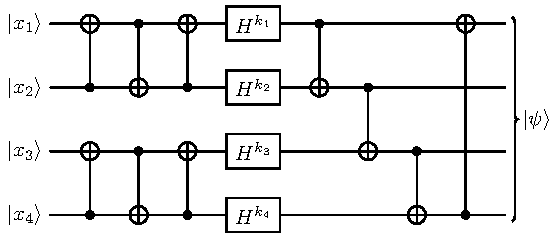
\includegraphics[page=1]{nsucrypto/problem10_figures.pdf}
\end{figure}

Plaintext 4 bit $(x_1, x_2, x_3, x_4)$ được biểu diễn ở dạng 4-qubit "plainstate" $\lvert x1, x2, x3, x4 \rangle$. Quantum state này là input cho mạch ở dạng qubit đơn đi qua các cổng.

Ở đây hai loại cổng được sửa dụng là CNOT và Hadamard.

Ký hiệu $H^b$ với $b \in \{ 0, 1 \}$ có nghĩa là, nếu $b = 0$ thì cổng đồng nhất $I$ được sử dụng (không thay đổi), còn nếu $b = 1$ thì cổng Hadamard sẽ được sử dụng.

Kết quả sau khi qua mạch là "cipherstate" $\lvert \psi \rangle$.

Bob có nhiệm vụ tăng số qubit đầu vào lên nhằm giảm các sai số khi tính toán và truyền dữ liệu trên kênh quantum. Do đó Bob biến đổi thành mạch sau:

\begin{figure}[ht]
    \centering
    \includegraphics[page=2]{nsucrypto/problem10_figures.pdf}
\end{figure}
Alice nói rằng cô ấy có thể tìm lại được key nếu biết $N$ amplitude của kết quả $\lvert \psi \rangle$. Do có 8 qubits ở kết quả nên số lượng amplitude tối đa là $2^8 = 256$, nói cách khác $N \leqslant 256$. Vậy Alice cần ít nhất bao nhiêu amplitude là đủ để tìm lại key?

\subsection*{Giải}

Đầu tiên xét 4 dây trên, 4 dây dưới tương tự.

\begin{figure}[ht]
    \centering
    \includegraphics[page=3]{nsucrypto/problem10_figures.pdf}
\end{figure}
Chúng ta xét dây 1 và 4 của mạch (tương tự cho dây 2 và 3). Áp dụng cổng CNOT liên tiếp 3 lần ta có
\begin{equation*}
    \lvert x_1 \rangle \otimes \lvert x_2 \rangle \to \lvert x_1 \oplus x_2 \rangle \otimes \lvert x_2 \rangle \to \lvert x_1 \oplus x_2 \rangle \otimes \lvert x_1 \rangle \to \lvert x_2 \rangle \otimes \lvert x_1 \rangle
\end{equation*}

\begin{figure}[ht]
    \centering
    \begin{subfigure}{0.3\textwidth}
        \includegraphics[page=4]{nsucrypto/problem10_figures.pdf}
        \caption{Dây 1 và dây 4}
    \end{subfigure}
    \begin{subfigure}{0.3\textwidth}
        \includegraphics[page=5]{nsucrypto/problem10_figures.pdf}
        \caption{Dây 2 và dây 3}
    \end{subfigure}
\end{figure}

Nói cách khác là đảo bit \emoji{grinning-squinting-face}.

Tương tự cho các cặp dây (5, 8) và (6, 7). Do đó khi tới trước các cổng Hadamard thì thứ tự các qubit từ trên xuống dưới là hình \ref{nsucrypto23:p10_4}.

\begin{figure}[ht]
    \centering
    \includegraphics[page=6]{nsucrypto/problem10_figures.pdf}
    \caption{Qubits trước Hadamard}
    \label{nsucrypto23:p10_4}
\end{figure}
Mạch ở dây 1 và 2 đều có dạng $\lvert x_2 \rangle$ đi qua $H^{k_1}$ nên sau khi qua cổng mình đặt $\lvert z_2 \rangle = H^{k_1} \lvert x_2 \rangle$.

Tương tự, $\lvert z_1 \rangle = H^{k_2} \lvert x_1 \rangle$ cho dây 3 và 4, $\lvert z_4 \rangle = H^{k_3} \lvert x_4 \rangle$ cho dây 5 và 6, $\lvert z_3 \rangle = H^{k_4} \lvert x_3 \rangle$ cho dây 7 và 8.

Mạch sau khi đi qua Hadamard có dạng \ref{nsucrypto23:p10_5}

\begin{figure}[ht]
    \centering
    \includegraphics[page=7]{nsucrypto/problem10_figures.pdf}
    \caption{Qubits sau Hadamard}
    \label{nsucrypto23:p10_5}
\end{figure}

Ở đây chúng ta có một lưu ý nhỏ có thể giúp ích trong việc giới hạn số lượng amplitude theo đề bài. Nếu $k_1 = 0$ thì $\lvert z_2 \rangle = \lvert x_2 \rangle$. Nếu $k_1 = 1$ thì $\lvert z_2 \rangle = \dfrac{\lvert 0 \rangle + (-1)^{x_2} \lvert 1 \rangle}{\sqrt{2}}$. Như vậy, hệ số trước $\lvert 0 \rangle$ của $\lvert z_2 \rangle$ có thể là $0, 1, \dfrac{1}{\sqrt{2}}$ đều không âm.

Bây giờ chúng ta quay lại toán tử CNOT. Ma trận tương ứng của toán tử CNOT là $\begin{pmatrix} 1 & 0 & 0 & 0 \\ 0 & 1 & 0 & 0 \\ 0 & 0 & 0 & 1 \\ 0 & 0 & 1 & 0 \end{pmatrix}$. Kết quả sau khi thực hiện toán tử CNOT là hệ số trước $\lvert 00 \rangle$ và $\lvert 01 \rangle$ giữ nguyên, còn hệ số trước $\lvert 10 \rangle$ và $\lvert 11 \rangle$ đổi chỗ cho nhau.

Đối với 3 qubit, mình \textbf{dự đoán} tương tự. 

Ở cổng CNOT đầu tiên, dây 1 control dây 3. Nếu mình chỉ xét 3 dây đầu thì tích các qubit gồm $\lvert 000 \rangle$, $\lvert 001 \rangle$, $\lvert 010 \rangle$, $\lvert 011 \rangle$, $\lvert 100 \rangle$, $\lvert 101 \rangle$, $\lvert 110 \rangle$, $\lvert 111 \rangle$. 

Áp dụng "chiến thuật" tương tự, mình chỉ quan tâm vị trí 1 và 3. Nghĩa là hệ số của $\lvert 0 x 0 \rangle$ và $\lvert 0 x 1 \rangle$ giữ nguyên, còn hệ số trước $\lvert 1 x 0 \rangle$ và $\lvert 1 x 1 \rangle$ đổi chỗ cho nhau, với $x \in \{ 0, 1 \}$. Nói cách khác, 8 hệ số trước amplitude chỉ thay đổi vị trí chứ không nhiều hơn hay ít đi, hay tập hợp hệ số giữ nguyên.

\begin{figure}[ht]
    \centering
    \includegraphics[page=8]{nsucrypto/problem10_figures.pdf}
\end{figure}

Như vậy, giả sử $\lvert z_2 \rangle = a \lvert 0 \rangle + b \lvert 1 \rangle$, $\lvert z_1 \rangle = c \lvert 0 \rangle + \lvert 1 \rangle$, $\lvert z_4 \rangle = e \lvert 0 \rangle + f \lvert 1 \rangle$, $\lvert z_3 \rangle = g \lvert 0 \rangle + h \lvert 1 \rangle$. Khi đó kết quả cipherstate là
\begin{equation*}
    \lvert \psi \rangle = \lvert z_2 \rangle \otimes \lvert z_2 \rangle \otimes \lvert z_1 \rangle \otimes \lvert z_1 \rangle \otimes \lvert z_4 \rangle \otimes \lvert z_4 \rangle \otimes \lvert z_3 \rangle \otimes \lvert z_3 \rangle
\end{equation*}

Xét $\lvert z_2 \rangle \otimes \lvert z_2 \rangle = a^2 \lvert 00 \rangle + ab \lvert 01 \rangle + ab \lvert 10 \rangle + b^2 \lvert 11 \rangle$. Ở đây có 3 hệ số khác nhau là $(a^2, ab, b^2)$. Với lưu ý bên trên $a \geqslant 0$ nên từ $a^2$ tính được $a$. Từ $a$, ta cần thêm $ab$ để xác định $b$.

Như vậy mình cần $2^4 = 16$ hệ số để tìm lại các key ban đầu.

\subsection*{Bình luận}

Thế éo nào mình lại nhầm khúc cuối mà lấy cả $a^2$, $ab$ và $b^2$ nên kết quả ra $3^4 = 81$. Tất nhiên là \textbf{SAI BÉT} nên chỉ được 2/8 \emoji{loudly-crying-face}.

\section*{Problem 11. AntCipher}
\addcontentsline{toc}{section}{Problem 11. AntCipher}

Bài này là bài số 2 ở round 1 và là bài số 11 ở round 2. Lúc thi round 1 mình không biết giải, còn ở round 2 thì mình đã giải theo cách như sau.

\subsection*{Đề bài}

Đặt
\begin{align*}
    f = (x_1 \lor x_2 \lor x_9) \land (\lnot x_1 \lor \lnot x_2 \lor \lnot x_9) \land (\lnot x_1 \lor x_2 \lnot x_9) \land (x_1 \lor \lnot x_2 \lor x_9) \land \\
    (x_1 \lor x_2 \lor x_3) \land (\lnot x_9 \lor \lnot x_{10} \lor \lnot x_3) \land (x_1 \lor \lnot x_2 \lor x_4) \land (\lnot x_9 \lor x_{10} \lor \lnot x_4) \land \\
    (\lnot x_1 \lor x_2 \lor x_5) \land (x_9 \lor \lnot x_{10} \lor \lnot x_5) \land (\lnot x_1 \lor \lnot x_2 \lor x_6) \land (x_9 \lor x_{10} \lor \lnot x_6) \land \\
    (x_1 \lor x_2 \lor x_3 \lor x_4 \lor \lnot x_7) \land (x_2 \lor x_3 \lor x_4 \lor \lnot x_7 \lor \lnot x_8)
\end{align*}

Hàm $f$ gồm 10 biến được viết dưới dạng CNF (conjunctive normal form). Thuật toán mã hóa dựa trên hàm $f$ biến đối hai bit plaintext $(x_1, x_2)$ thành hai bit ciphertext $(x_9, x_{10})$ khi giá trị hàm $f = True$. Hàm $f$ này có 10 biến $x_1, x_2, \ldots, x_{10}$ và 46 literals, là các hạng tử trong biểu diễn CNF của hàm. Ví dụ với dấu ngoặc thứ hai có 3 literals là $\lnot x_1$, $\lnot x_2$ và $\lnot x_9$.

\textbf{Q}. Vì các giới hạn tính toán nên chúng ta chỉ có thể sử dụng tối đa 16 biến với 20 literals. Nhắc lại rằng hàm $f$ ở trên có 10 biến và 46 literals. Hãy tìm cách biểu diễn tương đương của thuật toán mã hóa trên với giới hạn đã cho.

\subsection*{Giải}

Khi mình code hàm để tính giá trị hàm $f$ và xem xét những vector \[ \bm{x} = (x_1, \ldots, x_{10}) \] mà $f = True$, mình nhận thấy rằng:

\begin{itemize}
    \item nếu $(x_1, x_2) = (0, 0)$ thì $(x_9, x_{10}) = (1, 0)$
    \item nếu $(x_1, x_2) = (0, 1)$ thì $(x_9, x_{10}) = (1, 1)$
    \item nếu $(x_1, x_2) = (1, 0)$ thì $(x_9, x_{10}) = (0, 0)$
    \item nếu $(x_1, x_2) = (1, 1)$ thì $(x_9, x_{10}) = (0, 1)$
\end{itemize}

Mình nhận ra rằng các biến $x_3, x_4, \ldots, x_7, x_8$ hoàn toàn không tác động lên việc mã hóa từ $(x_1, x_2)$ thành $(x_9, x_{10})$ (ít nhất là ở những chỗ $f = True$ :v).

Như vậy bài toán được rút gọn thành hàm boolean 4 biến $x_1$, $x_2$, $x_9$ và $x_{10}$. Ở đó $f(0010) = f(0111) = f(1000) = f(1101) = 1$. Các vector còn lại thì $f=0$. Ở dưới là bảng chân trị \ref{nsucrypto23:prob11}.

\begin{table}[ht]
    \centering
    \begin{tabular}{|c|c|c|c|c|}
        \hline
        $x_1$ & $x_2$ & $x_9$ & $x_{10}$ & $f$ \\ \hline
        0 & 0 & 0 & 0 & 0 \\ \hline
        0 & 0 & 0 & 1 & 0 \\ \hline
        0 & 0 & 1 & 0 & 1 \\ \hline
        0 & 0 & 1 & 1 & 0 \\ \hline
        0 & 1 & 0 & 0 & 0 \\ \hline
        0 & 1 & 0 & 1 & 0 \\ \hline
        0 & 1 & 1 & 0 & 0 \\ \hline
        0 & 1 & 1 & 1 & 1 \\ \hline
        1 & 0 & 0 & 0 & 1 \\ \hline
        1 & 0 & 0 & 1 & 0 \\ \hline
        1 & 0 & 1 & 0 & 0 \\ \hline
        1 & 0 & 1 & 1 & 0 \\ \hline
        1 & 1 & 0 & 0 & 0 \\ \hline
        1 & 1 & 0 & 1 & 1 \\ \hline
        1 & 1 & 1 & 0 & 0 \\ \hline
        1 & 1 & 1 & 1 & 0 \\ \hline
    \end{tabular}
    \caption{Bảng chân trị hàm $f$}
    \label{nsucrypto23:prob11}
\end{table}

Từ bảng chân trị trên, sử dụng phương pháp bìa Karnaugh mình rút gọn được thành
\begin{align*}
    f(x_1, x_2, x_9, x_{10}) = & (\lnot x_1 \lor \lnot x_9) \land (x_1 \lor x_9) \land \\ 
    & (\lnot x_1 \lor \lnot x_2 \lor x_{10}) \land (x_1 \lor x_2 \lor \lnot x_{10}) \land \\
    & (\lnot x_1 \lor x_2 \lor \lnot x_{10}) \land (x_1 \lor \lnot x_2 \lor x_{10})
\end{align*}

CNF này có 4 biến và 16 literals, thỏa mãn yêu cầu đề bài và ăn trọn 6/6 điểm \emoji{smiling-face-with-halo}.



\chapter{Olympiad}

\section{Ôn thi ngày 20/11/2023}

\subsection*{Toán tử tuyến tính}

Toán tử tuyến tính là một ánh xạ \[ A: \RR^n \to \RR^m \]

Nếu $A$ là một ma trận cỡ $m \times n$ thì đây là một ánh xạ tuyến tính với phép nhân ma trận với vector $A \cdot \bm{x} = \bm{y}$.

Ở đây $\bm{x} \in \RR^n$ và $\bm{y} \in \RR^m$.

\begin{definition}[Hạt nhân]
    \textbf{Hạt nhân} của ánh xạ tuyến tính $A$ là tập hợp nghiệm của hệ thuần nhất và được ký hiệu là $\ker(A)$. Nói cách khác
    \begin{equation}
        \ker(A) = \{ \bm{x} \in \RR^n: \, A \cdot \bm{x} = \bm{0} \}
    \end{equation}
\end{definition}

\begin{definition}[Ảnh]
    \textbf{Ảnh} của ánh xạ tuyến tính $A$ là tập hợp tất cả giá trị có thể của phép nhân ma trận và được ký hiệu là $\Ima(A)$. Nói cách khác
    \begin{equation}
        \Ima(A) = \{ A \cdot \bm{x}: \, \bm{x} \in \RR^n \}
    \end{equation}
\end{definition}

Tính chất đối với ánh xạ $A: \RR^n \to \RR^m$ là $\dim(\ker A) + \dim(\Ima A) = n$.

\subsection*{Trị riêng và vector riêng}

\begin{definition}[Trị riêng, vector riêng]
    Xét hệ phương trình tuyến tính thuần nhất biểu diễn bởi phép nhân \[ A \cdot \bm{x} = \lambda \cdot \bm{x} \]

    Giá trị $\lambda$ khiến phương trình có nghiệm không tầm thường được gọi là \textbf{trị riêng} (eigenvalue) của ánh xạ tuyến tính.

    Vector $\bm{x}$ là cơ sở của không gian vector nghiệm khi đó được gọi là \textbf{vector riêng} (eigenvector) ứng với trị riêng $\lambda$.
\end{definition}

Lưu ý rằng có thể có nhiều vector riêng tương ứng với một trị riêng.

Để tìm trị riêng ta giải phương trình đặc trưng $\det (A - \lambda I) = 0$ và tìm tất cả nghiệm thực $\lambda$ của phương trình.

Sau đó ta thế từng $\lambda$ vào hệ $A \bm{x} = \lambda \bm{x}$ và tìm cơ sở của không gian nghiệm. Các vector trong cơ sở là vector riêng tương ứng với $\lambda$ đó.

Một số tính chất của trị riêng và vector riêng (giả sử rằng đối với ma trận $A$ cỡ $n \times n$ thì phương trình đặc trưng có đầy đủ $n$ nghiệm thực).

\begin{enumerate}
    \item $\tr A = \lambda_1 + \lambda_2 + \ldots + \lambda_n$
    \item $\det A = \lambda_1 \cdot \lambda_2 \cdots \lambda_n$
\end{enumerate}

Tính chất liên quan đến rank và trace:

\begin{enumerate}
    \item $\tr (AB) = \tr (BA)$
    \item $\rank (AB) \leqslant \min(\rank(A), \rank(B))$
\end{enumerate}

\subsection*{Bài tập}

\textbf{Bài 1}. Cho vector cột $\bm{v} \in \RR^n$. Đặt $A = \bm{v} \cdot \bm{v}^T$. Tìm $\spa A$.

Các cột của $A$ có dạng $\bm{v} \cdot v_1$, $\bm{v} \cdot v_2$, ..., $\bm{v} \cdot v_n$. Như vậy các cột đều tỉ lệ với cột đầu nên $\rank A = 1$.

Suy ra $\dim \ker A = n-1$ và do đó $\lambda = 0$ là nghiệm bậc $n-1$ trong phương trình đặc trưng.

Như vậy phương trình đặc trưng còn một nghiệm $\lambda \neq 0$.

Do $(\bm{v} \cdot \bm{v}^T) \bm{x} = \lambda \bm{x} \Leftrightarrow \bm{v} (\bm{v}^T \cdot \bm{x}) = \lambda \bm{x}$.

Đặt $\bm{v}^T \cdot \bm{x} = \alpha$ thì $\alpha \bm{v} = \lambda \bm{x}$. Suy ra $\bm{x} = \bm{v}$ và do đó $\alpha = \lambda = \lVert \bm{v} \rVert^2$.

Vậy $\spa A = \{ \lVert \bm{v} \rVert^2, 0, 0, \ldots, 0\}$.

\hfill

\textbf{Bài 3}. Cho ma trận $A_{3 \times 3}$. Biết rằng $\tr A = \tr A^{-1} = 0$ và $\det A = 1$. Chứng minh rằng $A^3 = I$.

Phương trình đặc trưng có dạng $P_3(\lambda) = -\lambda^3 + a_2 \lambda^2 + a_1 \lambda + a_0$.

Theo tính chất trên thì $a_2 = \sum \lambda = \tr A = 0$.

Do $\lambda$ là trị riêng nên $A \bm{x} = \lambda \bm{x}$. Do $A$ khả nghịch nên $\dfrac{1}{\lambda} \bm{x} = A^{-1} \bm{x}$.

Nghĩa là $\dfrac{1}{\lambda}$ là trị riêng của ma trận $A^{-1}$. Suy ra $\dfrac{1}{\lambda_1} + \dfrac{1}{\lambda_2} + \dfrac{1}{\lambda_3} = \tr A^{-1} = 0$.

Từ đó suy ra $\lambda_1 \lambda_2 + \lambda_2 \lambda_3 + \lambda_3 \lambda_1 = 0$.

Cuối cùng $\det A = \lambda_1 \cdot \lambda_2 \cdot \lambda_3 = 1$.

Vậy phương trình đặc trưng là $P_3(\lambda) = -\lambda^3 + 1$. Theo định lý Cayley-Hamilton thì $P_3(A) = -A^3 + I = 0$, hay $A^3 = I$.

\hfill

\textbf{Bài 4}. Cho ma trận $A_{n \times n}$, $A_{ij} \geqslant 0$. Giả sử ma trận có đủ $n$ trị riêng thực. Chứng minh rằng $\lambda_1^k + \lambda_2^k + \ldots + \lambda_n^k \geqslant 0$ với mọi $k \in \NN$.

Ta thấy rằng với $k=1$ thì $\lambda_1 + \ldots + \lambda_n = \tr(A) \geqslant 0$.

Vì $\lambda_i$ là thỏa phương trình $A \bm{x} = \lambda_i \bm{x}$ nên nhân hai vế cho $A$ ta có $A \cdot A \bm{x} = A \cdot \lambda_i \bm{x}$. Tương đương với $A^2 \bm{x} = \lambda_i (A \bm{x}) = \lambda_i^2 \bm{x}$.

Nói cách khác, $\lambda_i^2$ là trị riêng của ma trận $A^2$. Thực hiện tương tự ta có $\lambda_i^k$ là trị riêng của ma trận $A^k$.

Do đó $\lambda_1^k + \ldots + \lambda_n^k = \tr(A^k) \geqslant 0$.

\hfill

\textbf{Bài 5}. Cho ma trận $A$ khả nghịch. $X$ là ma trận sao cho $AX + XA = 0$. Chứng minh rằng $\tr X = 0$.

Nhân bên trái hai vế cho $A^{-1}$ ta có $X + A^{-1} X A = 0$. Ta biết rằng $A^{-1} X A$ là ma trận tương đương ma trận $X$ nên $\tr (A^{-1} X A) = \tr X$.

Suy ra $\tr X + \tr X = \tr 0 = 0$. Từ đây có $\tr X = 0$.

\section{RUDN Olympiad 2023}

Lần đầu tiên mình được tham dự thi toán đồng đội theo hình thức MathBoy (trận chiến toán).

Trong cách thi này, mỗi đội có 3 vị trí: người thuyết trình (докладчик), người phản biện (оппонент) và người giám sát (наблюдатель).

Ở mỗi vòng sẽ có 3 đội thi với nhau. Mỗi đội sẽ có 1 vị trí tương ứng với 3 vị trí trên. Sau đây là ví dụ

\begin{table}[ht]
    \centering
    \begin{tabular}{|c|c|c|c|}
        \hline
        & Đội 1 & Đội 2 & Đội 3 \\ \hline
        Vòng 1 & О & Д & Н \\ \hline
        Vòng 2 & Н & О & Д \\ \hline
        Vòng 3 & Д & Н & О \\ \hline
    \end{tabular}
\end{table}

Ở mỗi vòng, đội đóng vai trò người thuyết trình lên bảng ghi bài giải trong thời gian cho phép và thuyết trình về bài giải của đội mình. Đội phản biện có nhiệm vụ phản biện bài thuyết trình đó. Đội giám sát, dựa trên bài thuyết trình cũng như phản biện mà ghi chép lại các lỗi, chỗ khó hiểu, ... và trình lên cho giám khảo.

Ngoài ra, đội thuyết trình trước đó phải trình bài giải viết tay cho giám khảo chấm trước khi lên thuyết trình.

Ở đây có rất nhiều câu chuyện hack não đã xảy ra. Lúc mình thi vòng 1, câu hỏi quá khó nên đội thuyết trình chỉ viết được một ít. Đồng nghĩa việc đội phản biện cũng như đội giám sát ... thất nghiệp, không có gì để nói.

Đối với vòng 2, trận chiến cân bằng hơn, đội mình làm việc giám sát. Dựa trên bài giải của đội thuyết trình, chúng mình thấy những trường hợp chưa được xét tới và có thể bị sai, do đó cả ba đội đều có điểm (đội thuyết trình có nhiều điểm nhất vì các bạn giải hơn 1 nửa rồi).

Đối với vòng 3, đội mình thuyết trình. Đội mình clear bài đó nên giành điểm tuyệt đối cho phần thuyết trình. Tuy nhiên các bạn phản biện cũng không vừa, vẫn cố gắng bắt một số lỗi do trình bày quá cô đọng. Kết quả là đội mình (thuyết trình) full điểm cho vòng 3, đội phản biện được 3 điểm.

\section{Internet Olympiad Toán LB Nga 2023}

Giải này mình cay vl nên ngồi chép lại bài giải. Haizz.

\begin{problem}[Bài 1]
    Ở công viên cho trò chơi, với 5 dollar chúng ta được chơi 3 lượt
    và được thưởng 1 viên kẹo. Nếu trả lại 2 lượt (không chơi) thì
    chúng ta được trả lại 3 dollar đồng thời thêm 1 viên kẹo nữa.
    Ở đây không có quy luật trao đổi khác. Một đứa trẻ vào chơi,
    chỉ mang mỗi dollar. Kết thúc trò chơi, lượng dollar giảm
    nhưng đứa trẻ có 50 viên kẹo (không còn lượt chơi sót lại). 
    Hỏi đứa trẻ đã dùng bao nhiêu dollar cho trò chơi.
\end{problem}

\begin{solution}
    Đặt $x$ là số dollar ban đầu đứa trẻ có, và $y$ là số lượt 5 dollar mà đứa trẻ mua, tương đương $y$ viên kẹo. Suy ra số lần chơi mà đứa trẻ bỏ lại 2 lượt là $50-y$. 
    
    Nếu chơi hết 3 lượt thì đứa trẻ mất 5 dollar, nếu chơi 1 lượt (trả lại 2) thì đứa trẻ mất  $5-3=2$ dollar. Theo giả thiết là không còn lượt chơi sót lại, như vậy số lần chơi hết 3 lượt phải bằng bù lại số lần bỏ 2 lượt.
    
    Nói cách khác $3y = 2(50-y)$. Vậy $y=20$ và $50-y=30$. Nghĩa là số lần đứa trẻ trả lại 2 lượt chơi là $3 \cdot 30 = 90$ dollar, và số tiền trả là $5 y = 100$. Như vậy để có 50 viên kẹo thì đứa trẻ cần $100 - 90 = 10$ dollar.
\end{solution}

\begin{problem}[Bài 2]
    Gọi $x_0$ là cực tiểu địa phương của hàm số khả vi $f(x)$ thỏa mãn $f'(x) = 1 - x f^2(x)$ với mọi $x$. Hỏi có thể xác định nó là cực đại hay cực tiểu không?
\end{problem}

\begin{solution}
    Có thể. Do $x_0$ là cực trị địa phương nên $f'(x_0) = 0$.
    Suy ra $f'(x_0) = 1 - x_0 f^2(x_0) = 0$ và dễ thấy $x_0 = 0$
    không là nghiệm của phương trình. Vậy ta có $f^2(x_0) = \frac{1}{x_0} > 0$.

    Từ $f'(x) = 1 - x f^2(x)$ ta đạo hàm 2 vế thu được $f''(x) = -f^2(x) - 2xf(x) f'(x)$. 
    
    Do $f'(x_0) = 0$ nên $f''(x_0) = -f^2(x_0) - 2x_0 f(x_0) f'(x_0) = -f^2(x_0) < 0$.
    
    Suy ra $x_0$ là cực đại.
\end{solution}

\begin{problem}[Bài 4]
    Có bao nhiêu cách xếp 4 phần tử của 4 loại gạch khác nhau lên bảng 4x4 ô vuông sao cho ở mỗi hàng và mỗi cột có đúng 4 viên gạch thuộc 4 loại khác nhau?
\end{problem}

\begin{solution}
    Ta cố định hàng đầu tiên của bảng là 1-2-3-4.
    \begin{figure}[htb]
        \centering
        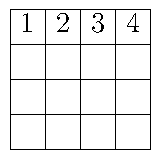
\includegraphics[page=1]{contests/internet_olympiad_figures.pdf}
    \end{figure}

    Tiếp theo ta bỏ các phần tử vào cột đầu theo thứ tự
    \begin{figure}[htb]
        \centering
        \includegraphics[page=2]{contests/internet_olympiad_figures.pdf}
    \end{figure}

    Trong bảng $3 \times 3$ còn lại ta phân bố các phần tử 1 vào các hàng, ta có 6 cách xếp như sau:
    \begin{figure}
        \centering
        \includegraphics[page=3]{contests/internet_olympiad_figures.pdf}
    \end{figure}

    Ta thấy rằng các trường hợp 1, 2, 4 và 6 sẽ có cách xếp các phần tử còn lại vào thỏa mãn. Nhưng trường hợp 3 và 5 sẽ bị đụng độ và không xếp được. Như vậy có 4 cách xếp.

    Với mỗi cách xếp, ta có thể hoán vị 3 phần tử ở cột đầu tiên (hàng đầu cố định, hoán vị từ hàng 2 tới 4) nên ta có $3!$ cách chọn. Với mỗi cách cố định hàng đầu ta có $4 \cdot 3!$ cách chọn, và ta có $4!$ cách xếp hàng đầu tiên.

    Như vậy kết quả là $4 \cdot 3! \cdot 4! = 576$.
\end{solution}

\begin{problem}[Bài 5]
    Cho hàm $f(x)$ thỏa mãn $f(x) + \dfrac{1}{2} \sin f(x) = x$ với mọi $x \in \RR$. Tính tích phân $\displaystyle{\int\displaylimits_{0}^{\pi} f(x)\,dx}$.
\end{problem}

\begin{solution}
    Đặt $t = f(x)$ thì $dt = f'(x)\,dx$. Sử dụng tích phân từng
    phần với $u = f(x)$ và $dv = dx$ ta có $du = f'(x)\,dx$ và
    $v = x$, suy ra:
    \[\int\displaylimits_{0}^{\pi} f(x)\,dx = x f(x) \Big|^\pi_0 - \int\displaylimits_{0}^{\pi}x f'(x)\,dx\]

    Từ giả thiết $f(x) + \dfrac{1}{2} \sin f(x) = x$, đạo hàm 2 vế ta có 
    \[f'(x) + \dfrac{1}{2} \cos f(x) f'(x) = 1,\]
    tương đương với $f'(x) = \dfrac{2}{2 + \cos f(x)}$ mà $-1 \leqslant \cos f(x) \leqslant 1$
    với mọi $x \in \RR$ nên $f'(x) > 0$ với mọi $x \in \RR$. Nghĩa
    là hàm đồng biến trên $\RR$.

    Từ đó, với mỗi $x \in \RR$ tồn tại duy nhất $f(x)$ tương ứng
    với nó. Ta thay $x = 0$ và $f(x) = 0$ vào phương trình thì 
    thấy thỏa mãn. Như vậy $f(0) = 0$. Tương tự $f(\pi) = \pi$.
    Do đó $x f(x) \Big|^\pi_0 = \pi^2$.

    Cũng từ đó ta có $\displaystyle{\int\displaylimits_{0}^{\pi} x f'(x)\,dx = \int\displaylimits_{0}^{\pi} x \, dt = \int\displaylimits_{0}^{\pi} (t + \dfrac{1}{2} \sin t)\,dt = \dfrac{\pi^2}{2} + 1}$.
    
    Tóm lại $\displaystyle{\int\displaylimits_{0}^{\pi}f(x)\,dx = \pi^2 - (\dfrac{\pi^2}{2} + 1)
    = \frac{\pi^2}{2} - 1}$.
\end{solution}

\begin{problem}[Bài 6]
    Trong không gian cho tam giác vuông cân $ABC$. 
    
    Gọi $A_1 B_1 C_1$ là hình chiếu của tam giác $ABC$ lên mặt phẳng nào đó ($A_1$, $B_1$, $C_1$
    lần lượt là hình chiếu của $A$, $B$ và $C$ lên mặt phẳng đó).
    Biết rằng $A_1 B_1 C_1$ cũng là tam giác vuông cân. Tìm mọi giá
    trị có thể của tỉ số giữa độ dài cạnh góc vuông $AB$ và cạnh
    góc vuông $A_1 B_1$
\end{problem}

\begin{solution}
    Không mất tính tổng quát, ta chọn $A_1$ ở gốc tọa độ $Oxyz$, 
    $B_1 = (1, 0, 0)$ và $C_1 = (0, 1, 0)$. Khi đó $A_1$ là hình
    chiếu của $A$ lên mặt phẳng $Oxy$ nên $A = (0, 0, 1)$. Tương
    tự, $B_1$ là hình chiếu của $B$ lên mặt $Oxy$ nên $B$ nằm
    trên đường thẳng qua $B$ song song $Oz$, vậy $B = (1, 0, x)$.
    Tương tự $C = (0, 1, y)$.

    Từ giả thiết $AB$ và $A_1 B_1$ là cạnh góc vuông, vậy $\angle A = 90$
    hoặc $\angle B = 90$.

    Ta có các vector $\overline{AB} = (1, 0, x-1)$, $\overline{AC} = (0, 1, y-1)$,
    $\overline{BC} = (-1, 1, y-x)$.
    Tương tự $\overline{A_1 B_1} = (1, 0, 0)$, $\overline{A_1 C_1} = (0, 1, 0)$,
    $\overline{B_1 C_1} = (-1, 1, 0)$.

    \textit{Trường hợp 1.} Tam giác $ABC$ vuông tại $A$. Khi đó
    $\overline{AB} \cdot \overline{AC} = 0$ và $\lvert \overline{AB}
    \rvert = \lvert \overline{AC} \rvert$. Tương đương với $(x-1)(y-1) = 0$
    và $1 + (x-1)^2 = 1 + (y-1)^2$. Suy ra $x = y = 1$. Như vậy 
    $\dfrac{AB}{A_1 B_1} = 1$.

    \textit{Trường hợp 2.} Tam giác $ABC$ vuông tại $B$. Khi đó
    $\overline{AB} \cdot \overline{BC} = 0$ và $\lvert \overline{AB} \rvert
    = \lvert \overline{BC} \rvert$. Tương đương với $-1 + (x-1)(y-x) = 0$
    và $1 + (x-1)^2 = 2 + (y-x)^2$. Ta thấy $x = 1$ không là nghiệm
    của phương trình đầu, nên $y - x = \dfrac{1}{x-1}$. Thay vào phương
    trình thứ hai và biến đổi ta có
    \begin{align*}
        & 1 + (x-1)^2 = 2 + \frac{1}{(x-1)^2} \\ 
        \Leftrightarrow & (x-1)^4 - (x-1)^2 - 1 = 0 \\ 
        \Leftrightarrow & (x-1)^2 = \frac{1+\sqrt{5}}{2}
    \end{align*}
    mà $AB = \sqrt{1 + (x-1)^2} = \sqrt{1 + \dfrac{1 + \sqrt{5}}{2}}
    = \dfrac{1 + \sqrt{5}}{2}$ và $A_1 B_1 = 1$ nên tỉ số là 
    $\dfrac{AB}{A_1 B_1} = \dfrac{1 + \sqrt{5}}{2}$

    Như vậy có 2 đáp án thỏa mãn là 1 và $\dfrac{1 + \sqrt{5}}{2}$.
\end{solution}

\begin{problem}[Bài 7]
    Cho hai ma trận vuông $A$ và $B$ sao cho $B^2 = 0$ và
    $A^2 B + B A^2 = 2A^3$. Chứng minh rằng với mỗi ma trận
    $A$ như vậy thì $A^{12} = 0$.
\end{problem}

\begin{solution}
    Từ giả thiết $A^2 B + B A^2 = 2A^3$, nhân hai vế của phương
    trình cho $B$ vào bên trái thì ta có $B A^2 B = 2BA^3$. Tương
    tự nếu nhân $B$ vào bên phải thì $B A^2 B = 2A^3 B$. Như vậy
    $BA^3 = A^3 B$.

    Tiếp theo nhân hai vế $A^2 B + B A^2 = 2A^3$ vào bên trái và bên
    phải cho $A^2$ thì $A^4 B + A^2 B A^2 = 2A^5$ và $A^2 B A^2 
    + BA^4 = 2A^5$. Như vậy $A^4 B = B A^4$.

    Khi đó $A^5 B = A \cdot A^4 B = A \cdot BA^4 
    = A \cdot BA^3 \cdot A = A \cdot A^3 B \cdot A 
    = A^4 B \cdot A = B A^4 A = B A^5$. Như vậy $A^5 B = B A^5$.

    Bình phương hai vế $A^2 B + BA^2 = 2A^3$ ta có
    \begin{align*}
        4A^6 & = A^2 B A^2 B + A^2B BA^2 + BA^2 A^2 B + BA^2 BA^2 \\
            & = A^2 B A^2 B + BA^4 B + BA^2 BA^2
    \end{align*}
    mà $BA^4B = A^4 B B = 0$ nên $4A^6 = A^2B A^2B + BA^2 BA^2$.

    Tiếp theo, từ $A^2 B + BA^2 = 2A^3$ ta có
    \begin{align*}
        A^2B A^2B & = A^2B (2A^3 - BA^2) = 2 A^2 B A^3 - A^2 B \cdot BA^2
                \\ & = 2 A^2 A^3 B - 0 = 2 A^5 B
    \end{align*}
    , tương tự
    \begin{align*}
        BA^2 BA^2 & = (2A^3 - A^2B) BA^2 = 2A^3 BA^2 - A^2B \cdot BA^2
                \\ & = 2 BA^3 \cdot A^2 - 0 = 2BA^5
    \end{align*}

    Mà $A^5 B = BA^5$ nên $4A^6 = 2A^5B + 2BA^5 = 4A^5B$. Suy ra
    $A^6 = A^5 B$. Cuối cùng $A^{12} = A^6 \cdot A^6 = A^5B \cdot BA^5
    = 0$. Điều phải chứng minh.
\end{solution}

\begin{problem}[Bài 8]
    Cho ba số dương $a$, $b$, $c$ sao cho $\sin a \cdot \sin b \cdot
    \sin c = \dfrac{3}{\pi} \cdot abc$. Chứng minh rằng 
    $a + b + c > \dfrac{\pi}{6}$.
\end{problem}

\begin{solution}
    Do $a$, $b$, $c$ dương nên ta có thể chia 2 vế cho $abc$ và có
    $\dfrac{\sin a}{a} \cdot \dfrac{\sin b}{b} \cdot \dfrac{\sin c}{c} = \dfrac{3}{\pi}$.

    Xét hàm $f(x) = \ln (\dfrac{\sin x}{x})$. Do $a$, $b$, $c$ dương
    nên vế trái cũng dương, do đó ta chỉ cần xét các số trong khoảng
    $(0, \frac{\pi}{2})$ là đủ. Khi đó, đặt

    \[f(x) = \begin{cases} \ln\Bigl(\frac{\sin x}{x}\Bigr), \quad
        & 0 < x < \frac{\pi}{2} \\
        0, \quad & x = 0
    \end{cases}\]

    Từ giả thiết suy ra:
    \begin{align*}
        f(a) + f(b) + f(c) & = \ln \Bigl(\frac{\sin a}{a}\Bigr) 
        + \Bigl(\frac{\sin b}{b}\Bigr) + \Bigl(\frac{\sin c}{c}\Bigr) \\
        & = \ln\Bigl(\frac{\sin a}{a} \cdot \frac{\sin b}{b} 
        \cdot \frac{\sin c}{c}\Bigr) \\
        & = \ln\Bigl(\frac{3}{\pi}\Bigr) = f\Bigl(\frac{\pi}{6}\Bigr)
    \end{align*}

    Ta thấy $e^{f(x)} = \dfrac{\sin x}{x}$. Đạo hàm hai vế suy ra
    $e^{f(x)} f'(x) = \Bigl(\dfrac{\cos x}{x} - \dfrac{\sin x}{x^2}\Bigr)$.
    Vậy:
    \[f'(x) = \Bigl(\frac{\cos x}{x} - \frac{\sin x}{x^2}\Bigr)
    \cdot \frac{x}{\sin x} = \cot x - \frac{1}{x}\]

    Và đạo hàm cấp hai:
    \[f''(x) = \frac{-1}{\sin^2 x} + \frac{1}{x^2}\]
    mà trên khoảng $(0, \dfrac{\pi}{2})$ thì $\sin x < x$
    nên $f''(x) < 0$ với mọi $x \in (0, \dfrac{\pi}{2})$.
    Do đó $f'(x)$ nghịch biến biến trên $(0, \dfrac{\pi}{2})$,
    và do $\dfrac{\sin x}{x}$ nghịch biến trên $(0, \dfrac{\pi}{2})$
    nên $f(x)$ cũng nghịch biến trên $(0, \dfrac{\pi}{2})$.

    Không mất tính tổng quát giả sử $a \leqslant b \leqslant c$.
    Theo định lý Lagrange (khúc này hack não lắm!!!) thì
    tồn tại số $\xi_1 \in (0, a)$ sao cho $f(a) - f(0) = 
    f'(\xi_1) \cdot (a - 0) \Leftrightarrow f(a) - f(0) = f'(\xi_1) \cdot a$.
    Tương tự tồn tại số $\xi_2 \in (a, a+b)$ sao cho
    $f(a+b) - f(b) = f'(\xi_2) \cdot (a + b - b) = f'(\xi_2) \cdot a$.

    Do $\xi_1 < \xi_2$ và $f'(x)$ nghịch biến nên $f'(\xi_1) > f'(\xi_2)$.
    Suy ra $f(a) - f(0) > f(a+b) - f(b)$, hay 
    $f(a) + f(b) > f(a+b) + f(0)$.

    Chứng minh tương tự ta cũng có $f(a+b) + f(c) > f(a+b+c) + f(0)$.
    Như vậy $f\Bigl(\frac{\pi}{6}\Bigr) = 
    f(a) + f(b) + f(c) > f(a+b) + f(0) + f(c) 
    > f(a+b+c) + f(0) + f(0) > f(a + b + c)$. 
    Do $f(x)$ nghịch biến nên $a + b + c > \dfrac{\pi}{6}$ là điều
    cần chứng minh.
\end{solution}

\begin{problem}[Bài 10]
    Cho đa thức với hệ số nguyên
    \[P_n(x) = a_n x^n + a_{n-1} x^{n-1} + \ldots + a_1 x + a_0\]

    Biết rằng $a_n$ là số lẻ, và $P_n(k)$, $P_n(k+1)$ là các số
    lẻ với $k$ nào đó. Chứng minh rằng đa thức không có nghiệm hữu tỷ.
\end{problem}

\begin{proof}
    Giả sử đa thức có nghiệm hữu tỷ $\dfrac{p}{q}$ với $p$ và $q$
    nguyên tố cùng nhau (phân số tối giản). Khi đó 
    $P_n(x) = \Bigl(x - \dfrac{p}{q}\Bigr) \cdot Q_{n-1}(x)
    = (qx - p) \Bigl(\dfrac{1}{q} Q_{n-1}(x)\Bigr)$.
    Do $p$ và $q$ nguyên tố cùng nhau nên $\dfrac{1}{q} Q_{n-1}(x)$
    cũng là một đa thức hệ số nguyên. Ta nhận thấy rằng
    \begin{align*}
        P_n(x) & = a_n x^n + a_{n-1} x^{n-1} + \ldots + a_1 x + a_0 \\
    & = (qx - p) \Bigl(\dfrac{a_n}{q} x^{n-1} + \ldots + \dfrac{-a_0}{q}\Bigr)
    \end{align*}
    
    Ở đây ta có thể xét hệ số bậc cao nhất và thấp nhất, và từ
    đó suy ra $\dfrac{a_n}{q}$ và $\dfrac{a_0}{q}$ là các số nguyên.

    Vậy với số nguyên $m$ bất kì thì $\dfrac{P_n(m)}{qm - p} = N(m)$
    cũng là một số nguyên. Mà từ giả thiết $a_n$, $P_n(k)$ và 
    $P_n(k+1)$ là các số lẻ thì $qk - p = 2m_1 - 1$ (số lẻ không
    thể chia hết cho số chẵn). Tương tự $q(k+1) - p = 2m_2 - 1$.
    Trừ vế theo vế ta có $(2m_2 - 1) - (2m_1 - 1) = 
    2 (m_2 - m_1) = q$. Như vậy $q$ là số chẵn, tuy nhiên do 
    $\dfrac{a_n}{q}$ là số nguyên và $a_n$ là số lẻ nên $q$ 
    phải là số lẻ, mâu thuẫn. 

    Theo phản chứng, đa thức không có nghiệm hữu tỷ.
\end{proof}

\chapter{RUDN Olympiad 2023}

Lần đầu tiên mình được tham dự thi toán đồng đội theo hình thức MathBoy (trận chiến toán).

Trong cách thi này, mỗi đội có 3 vị trí: người thuyết trình (докладчик), người phản biện (оппонент) và người giám sát (наблюдатель).

Ở mỗi vòng sẽ có 3 đội thi với nhau. Mỗi đội sẽ có 1 vị trí tương ứng với 3 vị trí trên. Sau đây là ví dụ

\begin{table}[ht]
    \centering
    \begin{tabular}{|c|c|c|c|}
        \hline
        & Đội 1 & Đội 2 & Đội 3 \\ \hline
        Vòng 1 & О & Д & Н \\ \hline
        Vòng 2 & Н & О & Д \\ \hline
        Vòng 3 & Д & Н & О \\ \hline
    \end{tabular}
\end{table}

Ở mỗi vòng, đội đóng vai trò người thuyết trình lên bảng ghi bài giải trong thời gian cho phép và thuyết trình về bài giải của đội mình. Đội phản biện có nhiệm vụ phản biện bài thuyết trình đó. Đội giám sát, dựa trên bài thuyết trình cũng như phản biện mà ghi chép lại các lỗi, chỗ khó hiểu, ... và trình lên cho giám khảo.

Ngoài ra, đội thuyết trình trước đó phải trình bài giải viết tay cho giám khảo chấm trước khi lên thuyết trình.

Ở đây có rất nhiều câu chuyện hack não đã xảy ra. Lúc mình thi vòng 1, câu hỏi quá khó nên đội thuyết trình chỉ viết được một ít. Đồng nghĩa việc đội phản biện cũng như đội giám sát ... thất nghiệp, không có gì để nói.

Đối với vòng 2, trận chiến cân bằng hơn, đội mình làm việc giám sát. Dựa trên bài giải của đội thuyết trình, chúng mình thấy những trường hợp chưa được xét tới và có thể bị sai, do đó cả ba đội đều có điểm (đội thuyết trình có nhiều điểm nhất vì các bạn giải hơn 1 nửa rồi).

Đối với vòng 3, đội mình thuyết trình. Đội mình clear bài đó nên giành điểm tuyệt đối cho phần thuyết trình. Tuy nhiên các bạn phản biện cũng không vừa, vẫn cố gắng bắt một số lỗi do trình bày quá cô đọng. Kết quả là đội mình (thuyết trình) full điểm cho vòng 3, đội phản biện được 3 điểm.



\chapter{Đường đoản thời}

\section*{Lời nói đầu}

Động lực để tác giả viết bài này là sau khi đọc về sự ra đời phép tính vi tích phân cùng vụ tranh cãi đáng xấu hổ trong lịch sử toán học giữa Newton và Leibniz, cùng với bài toán của Johann Bernoulli. 
        
Bài nghiên cứu này được tham khảo nhiều nguồn (từ Miguel A. Lerma\footnote{\emph{A simple derivation of the equation for the brachistochrone curve}, \url{https://sites.math.northwestern.edu/~mlerma/papers-and-preprints/brachistochrone.pdf}} và Lê Quang Ánh\footnote{\emph{Gia đình Bernoulli: một dòng họ Toán học}, trang 7, \url{https://rosetta.vn/lequanganh/gia-dinh-bernoulli-mot-dong-ho-toan-hoc/}}) và là tài liệu học tập cá nhân. Tác giả hy vọng rằng bài nghiên cứu nhỏ này sẽ giúp ích được cho các bạn học sinh, sinh viên đam mê toán và vật lý (mặc dù tác giả không phải dân lý hihi).

\section*{Bối cảnh lịch sử}

Thế kỷ 17 đã chứng kiến một drama có thể gọi là đáng xấu hổ nhất lịch sử toán học. Hai nhà toán học có ảnh hưởng rất lớn lại vướng vào một vụ kiện tụng và tranh cãi khó coi để xem ai là người phát minh ra phép tính vi tích phân. Vâng, chúng ta đang nói đến Newton và Leibniz. Vào thời điểm đó có một nhà toán học xuất sắc thuộc một dòng họ cũng gồm rất nhiều nhân vật xuất sắc đã đưa ra một bài toán đố cho các nhà toán học trên thế giới. Bài toán đó đã chứng minh được ưu thế vượt trội trong phương pháp vi tích phân của Leibniz.
    
Nhà toán học xuất sắc đó là Johann Bernoulli, thuộc dòng họ Bernoulli nổi tiếng. Bài toán đó được phát biểu như sau:
    
\textit{Cho hai điểm A và B nằm trong mặt phẳng thẳng đứng P (A cao hơn B). Hãy 
    xác định đường nối hai điểm A và B và nằm trong mặt phẳng P sao cho một 
    điểm chỉ chịu trọng lực chạy từ A đến B trong thời gian ngắn nhất.}

Chúng ta đã biết rằng đường đi ngắn nhất giữa hai điểm là đoạn thẳng nối hai điểm đó. Tuy nhiên trong bài toán của Johann Bernoulli thì đại lượng ngắn nhất cần tìm không phải khoảng cách giữa hai điểm mà là thời gian di chuyển giữa hai điểm. Mục tiêu cần làm ở bài toán này là xác định đường đi (hay quỹ đạo) thời gian ngắn nhất đó. Do đó bài toán này được gọi là bài toán \textit{đường đoản thời} (brachistochrone curve).

Để giải bài toán này chúng ta cần một định luật cũng về thời gian ngắn nhất. Đó là nguyên lý thời gian ngắn nhất của Fermat và một hệ quả của nó là định luật Snell-Descartes.

\section*{Định luật Snell-Descartes}

\begin{figure}[ht]
    \centering
    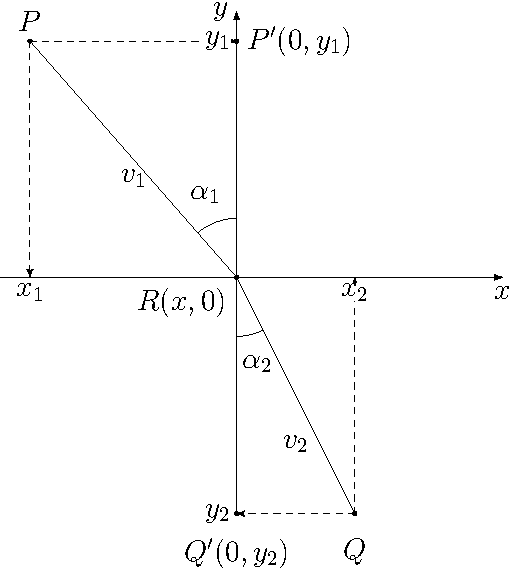
\includegraphics{brachistochrone/fermat.pdf}
    \caption{Định luật Snell-Descartes}
    \label{cycloid:snell}
\end{figure}

Nguyên lý thời gian ngắn nhất của Fermat phát biểu rằng

\textit{Khi ánh sáng truyền từ môi trường này sang môi trường khác thì nó luôn truyền đi theo đường nhanh nhất.}

Hệ quả của nguyên lý của Fermat là định luật Snell-Descartes mà chúng ta thường thấy ở chương trình vật lý ở phổ thông dưới dạng định luật khúc xạ ánh sáng
\begin{equation}
    \frac{\sin \alpha_1}{\sin \alpha_2} = \frac{v_1}{v_2}
\end{equation}
với $\alpha_1$ và $\alpha_2$ lần lượt là góc hợp bởi tia vào và tia ra với pháp tuyến tại điểm tới, $v_1$ và $v_2$ là vận tốc truyền trong môi trường ở nửa trên và nửa dưới $Ox$ (xem hình \ref{cycloid:snell}).

Để chứng minh định luật trên, ta thấy rằng $v_1$ là vận tốc khi di chuyển từ điểm $P$ tới điểm $R$ nên thời gian $t_1$ đi từ điểm $P$ tới $R$ là
\begin{equation}
    t_1 = \frac{\lVert \overrightarrow{PR} \rVert}{v_1} = \frac{\sqrt{(x - x_1)^2 + y_1^2}}{v_1}
\end{equation}

Lưu ý rằng tia sáng không truyền tới gốc tọa độ $O(0,0)$ mà truyền tới một điểm $R(x,0)$ là vì điểm bắt đầu là $P(x_1, y_1)$ và ánh sáng truyền đi theo đường nhanh nhất (theo nguyên lý Fermat) nên không có gì đảm bảo rằng nó sẽ truyền tới $O(0, 0)$.

Tương tự, thời gian $t_2$ đi từ điểm $R$ tới $Q$ là
\begin{equation}
    t_2 = \frac{\lVert \overrightarrow{RQ} \rVert}{v_2} = \frac{\sqrt{(x - x_2)^2 + y_2^2}}{v_2}
\end{equation}

Kết hợp hai phương trình của $t_1$ và $t_2$ lại thì tổng thời gian di chuyển từ $P$ tới $Q$ biểu diễn theo $x$ là
\begin{equation}
    T(x) = t_1 + t_2 = \frac{\sqrt{(x - x_1)^2 + y_1^2}}{v_1} + \frac{\sqrt{(x - x_2)^2 + y_2^2}}{v_2}
\end{equation}

Đạo hàm theo $x$ ta có
\begin{equation}
    T'(x) = \frac{x - x_1}{v_1 \sqrt{(x - x_1)^2 + y_1^2}} + \frac{x - x_2}{v_2 \sqrt{(x - x_2)^2 + y_2^2}}
\end{equation}

Để ý rằng $x > x_1$ nên $x - x_1 = \lVert \overrightarrow{PP'} \rVert$. Tương tự $x_2 - x = \lVert \overrightarrow{QQ'} \rVert$. Để tìm cực trị ta cho đạo hàm bằng 0 rồi tính đạo hàm cấp 2. Ta có
\begin{equation*}
    T'(x) = 0 \Leftrightarrow \frac{\lVert \overrightarrow{PP'} \rVert}{v_1 \lVert \overrightarrow{PR} \rVert} - \frac{\lVert \overrightarrow{QQ'} \rVert}{v_2 \lVert \overrightarrow{RQ} \rVert} = 0 \Leftrightarrow \frac{\sin \alpha_1}{v_1} - \frac{\sin \alpha_2}{v_2} = 0
\end{equation*}

Như vậy $\dfrac{\sin \alpha_1}{v_1} = \dfrac{\sin \alpha_2}{v_2}$. Đạo hàm cấp 2 tương ứng là
\begin{equation*}
    T''(x) = \frac{y_1^2}{v_1 ((x - x_1)^2 + y_1^2)} + \frac{y_2^2}{v_2 ((x - x_2)^2 + y_2^2)} > 0
\end{equation*}

Do đó $x$ thỏa $T'(x) = 0$ ở trên là cực tiểu và định luật Snell-Descartes được chứng minh.

\section*{Đường cong Cycloid}

Đáp án cho bài toán mà Johann Bernoulli đặt ra là đường cong Cycloid. Sau đây sẽ trình bày cách giải bài toán của Johann Bernoulli.

\begin{figure}[ht]
    \centering
    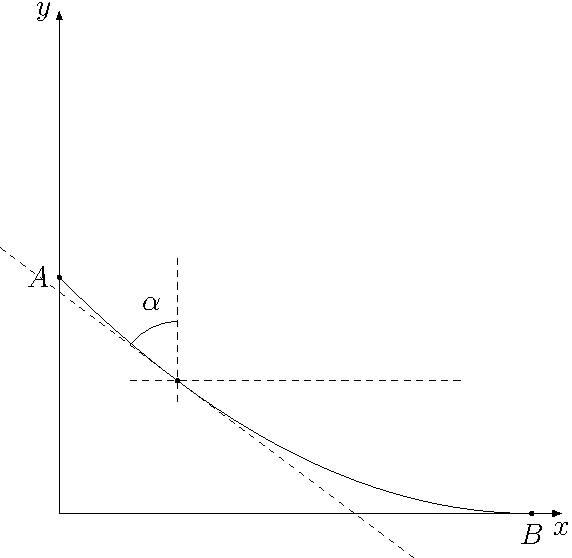
\includegraphics{brachistochrone/brachistochrone.pdf}
    \caption{Đường cycloid}
    \label{cycloid:im1}
\end{figure}

Phương của vận tốc tức thời tại một điểm khi một vật đi theo một quỹ đạo đường cong là tiếp tuyến với đường cong tại điểm đó. Khi đó góc $\alpha$ trong định luật Snell-Descartes sẽ có liên hệ với hệ số góc của tiếp tuyến với đường cong. Nói rõ hơn, góc hợp bởi tiếp tuyến và trục $Ox$ là $\alpha + \dfrac{\pi}{2}$ và hệ số góc của tiếp tuyến là $\tan \Bigl(\alpha + \dfrac{\pi}{2}\Bigr) = \dfrac{dy}{dx}$ (hình \ref{cycloid:im1}).

Ta có $\tan \Bigl( \alpha + \dfrac{\pi}{2} \Bigr) = -\cot \alpha$ và $1 + \cot^2 \alpha = \dfrac{1}{\sin^2 \alpha}$ nên 
\begin{equation}
    \dfrac{1}{\sin^2 \alpha} = 1 + \cot^2 \alpha = 1 + \Bigl(\dfrac{dy}{dx}\Bigl)^2
\end{equation}

Giả sử tọa độ của $A$ là $(x_0, y_0)$. Khi một điểm di chuyển từ $A$ tới $B$, gọi $(x, y)$ là tọa độ của điểm đó trên đường cong. Theo định luật bảo toàn cơ năng thì 
\begin{equation*}
    m g y_0 = \frac{1}{2} m v^2 + m g y
\end{equation*}
với $v$ là vận tốc tức thời tại điểm $(x, y)$ và $mgy$ là thế năng tại điểm đó. Như vậy ta có 
\begin{equation}
    v^2 = 2 g (-y + y_0)
\end{equation}

Theo định luật Snell-Descartes thì $\dfrac{v}{\sin \alpha}$ là một hằng số khi nằm trong cùng môi trường. Do đó tồn tại số $r$ cố định sao cho $\dfrac{v^2}{\sin^2 \alpha} = 4 g r$. Từ hai biểu thức của $v^2$ và $\dfrac{1}{\sin^2 \alpha}$ ở trên ta có
\begin{equation}
    \frac{v^2}{\sin^2 \alpha} = 2 g (-y + y_0) \Bigl( 1 + \Bigl(\frac{dy}{dx}\Bigr)^2 \Bigr) = 4 g r
\end{equation}

Suy ra
\begin{equation}
    \Big(\frac{dy}{dx}\Big)^2 = \frac{2 r}{y_0 - y} - 1
    \label{diff:eq1}
\end{equation}

Tới đây ta thấy rằng bậc của $dy$ và $dx$ ở vế trái là giống nhau, trong khi vế phải chỉ có $y$ mà không có $x$. Do đó "bắt chước" cách đổi biến của đường tròn, đặt
\begin{equation*}
    \begin{cases}
        x = a \theta + b \cos \theta \\
        y = c + d \sin \theta
    \end{cases}
\end{equation*}
với $a$, $b$, $c$, $d$ là các số thực cần tìm, $\theta$ là góc hợp bởi $Oy$ và đoạn thẳng nối tâm $O$ và điểm trên đường cong (theo góc $\alpha$). Lưu ý rằng khi thay $\theta = 0$ và $\theta = \pi / 2$ vào hai phương trình trên ta phải thu được hai điểm trên hai trục tọa độ.

Lấy vi phân hai phương trình trên ta có
\begin{equation*}
    \begin{cases}
    dx = a - b \sin \theta \, d \theta \\ dy = d \cos \theta \, d \theta
\end{cases}
\end{equation*}

Thay vào phương trình \ref{diff:eq1} ta được
\begin{equation*}
    \frac{d^2 \cos^2 \theta}{(a - b \sin \theta)^2} = \frac{2 r}{y_0 - c - d \sin \theta} - 1 = \frac{2 r - y_0 + c + d \sin \theta}{y_0 - c - d \sin \theta}
\end{equation*}

Do $\cos^2 \theta = 1 - \sin^2 \theta = (1 - \sin \theta)(1 + \sin \theta)$ nên ta muốn chọn $a$ và $b$ có thể rút gọn được cho tử số. 

\textbf{Trường hợp 1}. $a = b$, ta thu được
\begin{equation*}
    \frac{d^2 (1 + \sin \theta)}{a^2 (1 - \sin \theta)} = \frac{(2 r - y_0 + c) + d \sin \theta}{(y_0 - c) - d \sin \theta}
\end{equation*}

Ta sẽ muốn đồng nhất hệ số tự do và hệ số trước $\sin \theta$ để dễ tính toán sau này. Do đó một cách chọn đơn giản là $2 r - y_0 + c = d$ và $y_0 - c = d$. Suy ra $r = d$. Thu gọn phương trình ta được
\begin{equation*}
    \frac{d^2 (1 + \sin \theta)}{a^2 (1 - \sin \theta)} = \frac{1 + \sin \theta}{1 - \sin \theta}
\end{equation*}

Như vậy $a^2 = d^2$ nên $a = d$ hoặc $a = -d$. Ta xét trường hợp $a = d$, trường hợp $a = -d$ cũng cho kết quả tương tự (không thỏa mãn). 

Ta có  $a = b = d = r$ và $c = y_0 - d = y_0 - r$. Phương trình đường cong trong tọa độ cực sẽ là
\begin{equation*}
    \begin{cases}
        x = r(\theta + \cos \theta) \\ y = (y_0 - r) + r \sin \theta
    \end{cases}
\end{equation*}

Với $\theta = 0$ thì $(x, y) = (r, y_0 - r$. Với $\theta = \pi / 2$ thì $(x, y) = (\pi r / 2, y_0)$.

Tới đây chúng ta có thể thêm bớt một hằng số để "kéo" các tọa độ về trục. 

Ta đưa tọa độ khi $\theta = 0$ về $Oy$ thì $x' = x - r$. Tương tự tọa độ khi $\theta = \pi / 2$ sẽ về $Ox$ nên $y' = y - y_0$. Như vậy tọa độ (mới) cho hai trường hợp $\theta$ là $(0, -r)$ và $(\pi r / 2 - 1, 0)$ nhưng vì $r$ là số dương (bán kính) nên $(0, -r)$ nằm dưới trục $Ox$, không phù hợp với hình vẽ.

\textbf{Trường hợp 2}. $a = -b$, ta thu được
\begin{equation*}
    \frac{d^2 (1 - \sin\theta)}{a^2 (1 + \sin\theta)} = \frac{(2r - y_0 + c) + d \sin\theta}{(y_0 - c) - d \sin\theta}
\end{equation*}

Tương tự, để đồng nhất và rút gọn hệ số cho hợp với bên vế trái ta chọn $2r - y_0 + c = -d$ và $y_0 - c = -d$. Suy ra $d = -r$. Thu gọn phương trình ta được
\begin{equation*}
    \frac{d^2 (1 - \sin\theta)}{a^2 (1 + \sin\theta)} = \frac{1 - \sin\theta}{1 + \sin\theta}
\end{equation*}

Như vậy $a^2 = d^2$ nên $a = d$ hoặc $a = -d$ Ta xét trường hợp $a = -d$.

Khi đó $a = -b = -d = r$ và $c = y_0 + d = y_0 - r$. Phương trình đường cong trong tọa độ cực sẽ là 
\begin{equation*}
    \begin{cases}
        x = r (\theta - \cos\theta) \\
        y = (y_0 - r) - r \sin\theta
    \end{cases}
\end{equation*}

Với $\theta = 0$ thì $(x, y) = (-r, y_0)$. Với $\theta = \pi / 2$ thì $(x, y) = (r (\pi / 2 - 1), y_0 - 2r)$.

Tới đây ta cũng thêm bớt một hằng số vào hoành độ và tung độ để "kéo" các tọa độ về trục.

Ta đưa tọa độ khi $\theta = 0$ về $Oy$ thì $x' = x + r$. Tương tự ta đưa tọa độ khi $\theta = \pi / 2$ về $Ox$ thì $y' = y - y_0 + 2r$. Khi đó tọa độ (mới) là $(0, 2r)$ và $(\pi r / 2, 0)$. Điều này phù hợp với yêu cầu bài toán và tương đương với phương trình trong tọa độ cực 
\begin{equation}
    \begin{cases}
        x = r (\theta - \cos\theta) + r = r (1 + \theta - \cos\theta) \\
        y = (y_0 - r) - r \sin\theta - (y_0 - 2r) = r (1 - \sin\theta)
    \end{cases}, 0 \leq \theta \leq \frac{\pi}{2}
\end{equation}

Đây chính là kết quả cần tìm. Thêm nữa vị trí ban đầu của vật là $(0, y_0)$ và tọa độ theo phương trình là $(0, 2r)$ nên suy ra $y_0 = 2r$.

\section*{Phương trình phụ thuộc thời gian}

Trong phương trình đường cong có sự tham gia của bán kính $r$ cố định và góc quét $\theta$. Chúng ta cần mối liên hệ giữa các phương trình theo thời gian.

Nhắc lại, vận tốc tức thời tại một điểm có phương trùng với tiếp tuyến với đường cong tại điểm đó. Do đó $v = \dfrac{\sqrt{(dy)^2 + (dx)^2}}{dt}$ xác định vận tốc tức thời với quãng đường là $(dy)^2 + (dx)^2$ là bình phương khoảng cách trong mặt phẳng. Từ đây suy ra
\begin{align*}
    v^2 = \Bigl(\frac{dy}{dt}\Bigr)^2 + \Bigl(\frac{dx}{dt}\Bigr)^2 = r^2 \cos^2 \theta \Bigl( \frac{d \theta}{dt} \Bigr)^2 + r^2 (1 + \sin \theta)^2 \Bigl( \frac{d \theta}{dt} \Bigr)^2 \\ = 2 r^2 (1 + \sin \theta) \Bigl( \frac{d \theta}{dt} \Bigr)^2
\end{align*}

Từ bên trên và $y_0 = 2r$ ta có \[v^2 = 2 g (y_0 - y) = 2 g (y_0 - r + r \sin \theta) = 2 g r ( 1 + \sin \theta)\]

Suy ra
\begin{equation*}
    2 r^2 (1 + \sin \theta) \Bigl( \frac{d \theta}{dt} \Bigr)^2 = 2 g r (1 + \sin \theta)
\end{equation*}
Hay
\begin{equation}
    \Bigl(\frac{d \theta}{dt}\Bigr)^2 = \frac{g}{r} \Rightarrow \frac{d \theta}{dt} = \sqrt{\frac{g}{r}} = \text{const}
\end{equation}

Như vậy $\theta = \sqrt{\dfrac{g}{r}} t = \omega t$. Ở đây $t$ là thời gian tính từ lúc bắt đầu thả vật từ điểm $A$. Cuối cùng phương trình phụ thuộc thời gian của đường cong Cycloid là
\begin{equation}
    \begin{cases}
        x = r (1 + \omega t - \cos \omega t) \\ y = r (1 - \sin \omega t)
    \end{cases}
\end{equation}

Trong đó, $r$ là bán kính cố định (bằng nửa độ cao ban đầu $y_0$ của vật), $\omega = \frac{g}{r}$ là tần số góc, $y_0$ là độ cao ban đầu của vật (tung độ điểm $A$).

\printbibliography[title={Tài liệu tham khảo}]
\end{document}